\documentclass[12pt,a4paper]{article}
\usepackage[T1]{fontenc}
\usepackage[utf8]{inputenc}
\usepackage[left=2cm, right=2cm]{geometry}
\usepackage{afterpage}
\usepackage{tikz}
\usepackage{fancyhdr}
\usepackage{mathtools}
\usepackage{graphicx}
\usepackage{hyperref}
\usepackage{float}
\usepackage{booktabs, tabularx}
\usepackage{multicol}
\usepackage{caption}
\usepackage{eurosym}
\usepackage{biblatex}
\usepackage{multicol}
\usepackage{color}
\setlength\columnseprule{.5pt}
\bibliography{biblio.bib}

\setlength{\tabcolsep}{10pt}

\setlength{\parindent}{0pt}

\graphicspath{{img/}}

\DeclareRobustCommand{\rchi}{{\mathpalette\irchi\relax}}
\newcommand{\irchi}[2]{\raisebox{\depth}{\scalebox{1.2}{$#1\chi$}}}

\newcommand{\archtest}[3]{
\begin{equation*}
    \begin{split}
        H_{0} &: \text{Homoscédasticité} \\
        H_{1} &: \text{Hétéroscédasticité}
    \end{split}
\end{equation*}
Statistique de test :
    \begin{equation*}
        LM = n \times R^{2} \sim \rchi^{2}_{0,95} \, (p)
    \end{equation*}
La statistique du multiplicateur de Lagrange est comparée au quantile à 95\% de la distribution du khi-deux ayant pour degrés de liberté #1. Dans le cas suivant :}

\newcommand{\test}[3]{
    \begin{equation*}
        \begin{split}
            H_{0} &: \text{#1} \\
            H_{1} &: \text{#2}
        \end{split}
    \end{equation*}
    Statistique de test :
    \begin{equation*}
        #3
    \end{equation*}}


\usetikzlibrary{fadings}
\definecolor{light}{HTML}{E0E3C2}
\DeclareFixedFont{\titlefont}{T1}{ppl}{b}{n}{1.2cm}
\DeclareFixedFont{\subtitlefont}{T1}{ppl}{m}{n}{0.6cm}
\DeclareFixedFont{\namefont}{T1}{ppl}{m}{n}{0.6cm}

\begin{document}
\afterpage{\restoregeometry}
\newgeometry{left=1in, right=1in,top=1in, bottom=-0.5in}
\definecolor{mytan}{HTML}{1C3651}
\pagecolor{mytan}\afterpage{\nopagecolor}
\thispagestyle{empty}
\begin{center}

\includegraphics{um3.png} \hspace{5em} 
\includegraphics[scale=0.23]{eco.png} \par
\vfill
\titlefont \textcolor{light}{Projet d'économétrie appliquée}\par\vspace{0.5cm}
\subtitlefont \textcolor{light}{Comparaison de l'algorithme de Box et Jenkins aux méthodes de prévision traditionnelles pour la prévision de deux matières premières : le 
blé et le nickel}
\vfill
\namefont \textcolor{light}{Mosse Joseph - Rubira Pierre}\par\vspace{0.2cm}
\namefont \textcolor{light}{M1 - MBFA - ARB}
\vfill
\namefont \textcolor{light}{Sous la direction de :}\par\vspace{0.2cm}
\namefont \textcolor{light}{Seyte Françoise}
\end{center}

\begin{center}
\begin{tikzpicture}
\node[scope fading=north, inner sep=0pt, outer sep=0pt]{
 \makebox[\textwidth]{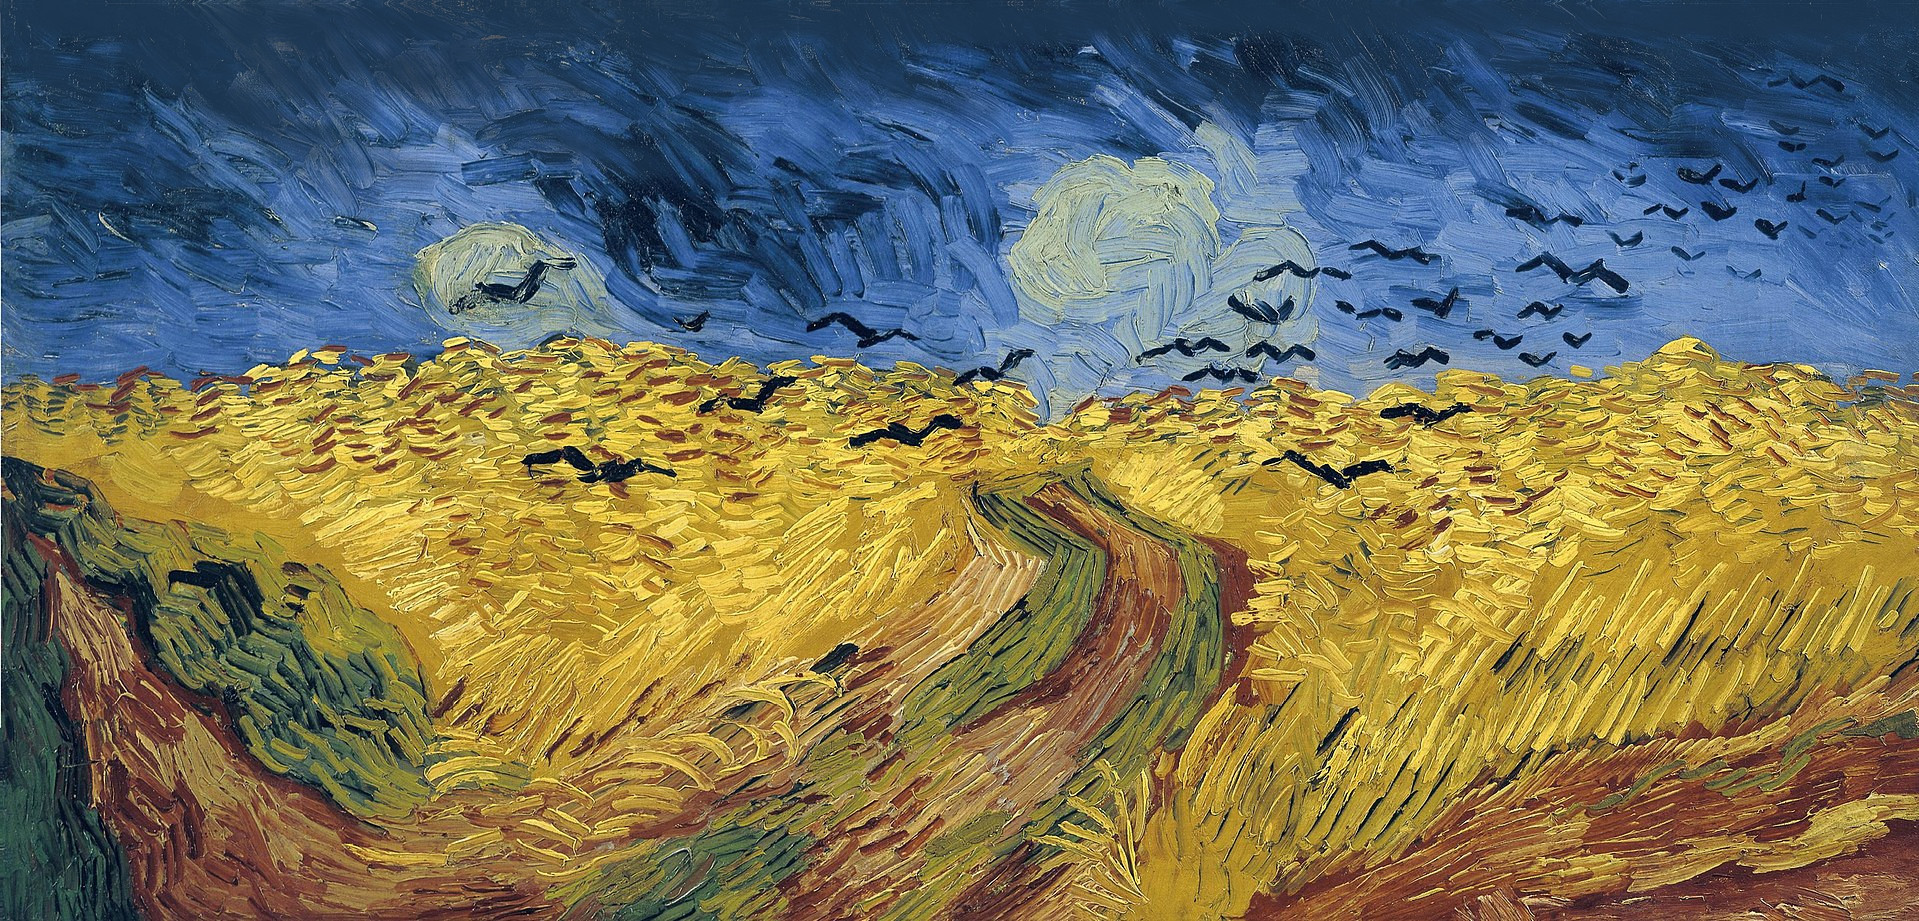
\includegraphics[width=\paperwidth]{ble2.jpg}}
};
\end{tikzpicture}
\end{center}

\clearpage
\newgeometry{left=2.5cm, right=2.5cm,top=2.5cm, bottom=2.5cm}
\pagenumbering{arabic}
\pagestyle{fancy}
\fancyhead{}
\fancyfoot[C]{\thepage}
\section*{Résumé}
\renewcommand\contentsname{Sommaire}
\tableofcontents



\section*{Introduction}
\section{Analyse technique et macroéconomique du blé et du nickel}
\subsection{Présentation des deux matières premières}
\subsection{Analyse macroéconomique}
\subsection{Analyse technique}

\section{Analyse des séries chronologiques}
Les méthodes traditionnelles de prévision, reposent sur la décomposition des différentes composantes d'une série temporelle. Ici il s'agira donc
ici d'analyser ces différentes composantes (c'est à dire la tendance et la saisonnalité).
\subsection{Stabilité de la variance}
Afin de pouvoir travailler sur la série, il est nécessaire de réduire les 
fluctuations importantes de la série. Pour cela des test ARCH sont fait sur les 
séries initiales afin de déterminer si il y a homoscédasticité dans la distribution. L'hypothèse nulle et alternative sont :
\archtest{41}{27,31}{14,07}
\begin{table}[H]
    \centering
    {\sffamily
    \begin{tabular}{lcc}
        \toprule
        Série           &  $LM$ & $\rchi^{2}_{0,95} (7)$\\
        \midrule
        Blé (16-19)     & 27,30     & 14,07 \\ 
        Blé (16-21)     & 54,10     & 14,07\\
        \bottomrule
    \end{tabular}
    \begin{tabular}{lcc}
        \toprule
        Série           &  $LM$ & $\rchi^{2}_{0,95} (7)$\\
        \midrule
        Nickel (16-19)  & 21,40     & 14,07\\
        Nickel (16-21)  & 49,96     & 14,07\\
        \bottomrule
    \end{tabular}}
    \caption{Résultats du test ARCH}
\end{table}
Ici, pour toutes les séries, la statistique $LM$ est supérieur au seuil, l'hypothèse $H_{0}$ est 
rejetée au risque de $5\%$. Les cours du blé et du nickel sont donc présente de l'hétéroscédasticité. Afin d'amoindrir ces fluctuations importantes, une transformation 
logarithmique est faite sur chacune des séries. Les séries transformées serviront donc
pour le reste du travail.

\subsection{Analyse graphique et tableau de Buys-Ballot}\label{graph}
Dans un premier temps, une étude intuitive peut être faite. Il s'agira donc ici d'analyser graphiquement chacune des chroniques afin 
de déterminer de façon préliminaire, si les cours du blé et du nickel sont sujet à de la saisonnalité, et/ou de la tendance.

Pour le cours du blé, il est possible de déceler légère une tendance a la hausse de 2016 à 2019. Cette tendance s'accentue si 2020 et 2021 
sont inclus. Pour ce qui est de la saisonnalité, il semble impossible de déterminer que la série possède une quelconque saisonnalité
\textit{(figure~\ref{fig:ble_log} p.~\pageref{fig:ble_log})}.

Dans le cas du nickel, une tendance haussière se démarque (tout échantillon confondu). Quant à la saisonnalité, sur l'échantillon 2016-2019, 
la série ne semble pas saisonnière. Cependant sur l'échantillon 2016-2021, la série peut sembler saisonnière par périodes de un an.
\textit{(figure~\ref{fig:nickel_log} p.~\pageref{fig:nickel_log})}.

Les deux séries semblent donc se comporter de manière similaire : faible tendance haussière, ainsi que non saisonnières. 

\subsection{Analyse de la variance}
Afin de confirmer les intuitons développées en ~\ref{graph} une analyse de la variance et le test de Fisher sur la tendance et de 
saisonnalité doivent être menés. La détection de la saisonnalité est essentielle, car les méthodes de prévision traditionnelles
ne peuvent être que menées sur des séries non saisonnières ou bien désaisonnalisées.

L'analyse de la variance est basée sur les moyennes calculées dans le tableau de Buys Ballot. En effet afin d'analyser la saisonnalité, 
il reviendra a étudier l'influence du facteur colonne (variance des mois) et pour la tendance, l'influence du facteur ligne (variance des années).
Après calculs \textit{(Cf-\ref{appendix:anova} p.\pageref{appendix:anova})}, les différentes variances sont affichées dans le tableau ci-dessous.

\begin{table}[H]
    \centering
    \caption{Analyse de la variance}
    \sffamily
    \begin{tabular}{lcccc}
\toprule
\multirow{2}*{Échantillon}& \multicolumn{2}{c}{2016-2019}   & \multicolumn{2}{c}{2016-2021} \\
      &  Blé &  Nickel& Blé &  Nickel \\ 
\cmidrule(r){1-1}\cmidrule(lr){2-3}\cmidrule(l){4-5}
    Variance période                         & 0,0086      &   0,0129    & 0,0023       & 0,0243      \\
    Variance année                           & 0,2746      &   0,3723    & 0,0661       & 0,6502      \\
    Variance résidus                         & 0,0048      &   0,0286    & 0,0033       & 0,0098      \\ 
\bottomrule
\end{tabular}
\end{table}

Enfin grace aux variances, le test de fisher peut être effectué.

\subsubsection{Test de Fisher de détection de saisonnalité}
Il s'agira ici de tester l'influence du facteur colonne en comparant la variance période à la variance résiduelle
,afin de déterminer si les séries sont saisonnières.
\test{Pas d'influence du facteur colonne (pas de saisonnalité)}
    {Influence du facteur colonne (saisonnalité)}
    {F_{c} = \frac{V_{P}}{V_{R}} \sim F_{0,95}((n-1), (n-1)(p-1))}
La statistique calculée ($F_{c}$) est ensuite comparée au quantile à $95\%$ de la distribution $F$ de
Fisher avec comme degrés de liberté $(p-1)$ et $(n-1)(p-1)$, où $n$ représente le nombre d'année
et $p$ le nombre de périodes. Si la statistique empirique est supérieure au quantile,
alors $ H_{0} $ est rejetée, la série est saisonnière. Après calculs :
\begin{table}[H]
    \centering
    \caption{Test de Fisher (saisonnalité)}
    \sffamily
    \begin{tabular}{lcccc}
\toprule
    & \multicolumn{2}{c}{2016 -2019}   & \multicolumn{2}{c}{2016 -2021} \\
    & Blé  & Nickel & Blé  & Nickel \\
  \cmidrule(r){1-1}\cmidrule(lr){2-3}\cmidrule(l){4-5}
  $F_{c}$ & 0,6986  & 0,4505  &  1,7906 & 2,4772                     \\ 
  $F_{0,95}$ & 2,0933 & 2,0933	& 1,9675 & 1,9675\\
  \textit{ddl} &  (11;33)& (11;33) & (11;55) & (11;55)\\
  \bottomrule             
\end{tabular}
\end{table}
Ici, les statistique calculée sont toutes inférieures au seuil, sauf pour l'échantillon (2016-2021)
du nickel.  Ainsi, l'hypothèse $H_{0}$ est acceptée au risque de $5\%$ pour les deux échantillons du blé
et pour l'échantillon (2016-2019) du nickel. En revanche elle est rejetée pour l'échantillon (2016-2021) du nickel.\\[11pt]
Pour ses deux échantillons, la série du blé n'est donc pas saisonnière, il en est de même pour le premier échantillon de la série du nickel. 
Par contre, l'échantillon (2016-2021) du nickel est lui saisonnier, il faudra donc à la suite 
déterminer son type de saisonnalité (déterministe ou aléatoire), puis son type de schéma de décomposition
(additif ou multiplicatif) et finalement désaisonnaliser la série afin de pouvoir utiliser les méthodes de prévision.
\subsubsection{Test de Fisher de détection de tendance}
De manière analogue, il revient à comparer la variance année à la variance résiduelle afin de déterminer si les séries possèdent une tendance.
\test{Pas d'influence du facteur ligne (pas de tendance)}
    {Influence du facteur ligne (tendance)}
    {F_{c} = \frac{V_{A}}{V_{R}} \sim F_{0,95}((p-1), (n-1)(p-1))}
Comme pour le test précédent, si la statistique calculée est supérieure au quantile à $ 95\% $ 
de la distribution de Fisher ayant pour \textit{dll} : $(n-1)$ et $(n-1)(p-1)$ , alors $ H_{0} $ est rejetée, la série possède une tendance.
\begin{table}[H]
    \centering
    \caption{Test de Fisher (tendance)}
    \sffamily
    \begin{tabular}{lcccc}
    \toprule
         & \multicolumn{2}{c}{2016 -2019} & \multicolumn{2}{c}{2016 -2021}  \\
         & Blé      & Nickel    & Blé       & Nickel                        \\
    \cmidrule(r){1-1}\cmidrule(lr){2-3}\cmidrule(l){4-5}
        $F_{c}$     & 20,1576   & 12,9965   & 56,8388   & 66,2263           \\
        $F_{0,95}$  & 2,8916    & 2,8916    & 2,3828    & 2,3828            \\*
        \textit{ddl}& (3;33)    & (3;33)    & (5;55)    & (3;55)            \\
    \bottomrule
\end{tabular}

\end{table}
Ici dans tous les cas, le Fisher empirique est supérieur au Fisher théorique, $H_{0}$ est rejetée
au risque de $ 5\% $ pour toutes les séries. \\[11pt]
Les deux séries et leurs échantillons possèdent donc une tendance. Il à remarquer que la probabilité de rejeter 
$H_{0}$ est bien plus supérieure sur les échantillons (2016-2021) que sur les échantillons (2016-2019),
cela confirme l'intuition dégagée de l'analyse graphique.

\subsection{Analyse de la saisonnalité de l'échantillon (2016-2021) du nickel}
Comme vu précédemment l'échantillon (2016-2021) du Nickel possède de la saisonnalité, il est donc indispensable d'étudier, puis de corriger la saisonnalité. 
\subsubsection{Type de saisonnalité et schéma de décomposition}
Dans un premier temps le type de saisonnalité doit être défini, en effet la saisonnalité peut être déterministe ou bien aléatoire. Pour cela chaque ligne du tableau de 
Buys-Ballot de l'échantillon concerné est classée par ordre croissant. De plus pour faciliter la lecture, chaque mois s'est vu attribué une couleur appartenant à
un gradient rouge (\textit{tableau~\ref{tab:bbc} p.\pageref{tab:bbc} }). Il est donc rapidement possible de remarquer que la saisonnalité n'est pas répétitive,
elle est donc aléatoire. Il faudra donc désaisonnaliser la série par méthode CENSUS.\\[11pt] 


\section{Prévision par le méthodes traditionnelles}\label{tradi}
Une fois que toutes les séries ont été amplement analysées, transformées, et si besoin, corrigées des variations saisonnières, il alors est possible d'appliquer des 
méthodes de prévision traditionnelles. Le choix d'une méthode de prévision depend du caractère déterministe (ou aléatoire) de l'extra-saisonnalité et de la saisonnalité de
la série a prévoir. \\[11pt]
Dans le cadre de l'étude du cours du blé et du nickel, il a précédemment été montré que les deux échantillons du blé, ainsi que l'échantillon 2016-2019 
du nickel ne présentaient pas de saisonnalité, pour ces séries là donc, seule la nature de la composante extra-saisonnière est à prendre en compte. Concernant cette 
dernière, elle est déterministe pour les trois séries citées étant donné qu'elles possèdent toutes une tendance. Dans ce cas là, en théorie la méthode de prévision a 
utiliser serait l'extrapolation par une droite de tendance.\\[11pt]
Concernant l'échantillon 2019-2021 du nickel, malgré une composante saisonnière aléatoire, ce dernière possède comme les autres échantillons, une tendance. La méthode de 
prévision adéquate serait donc aussi l'extrapolation d'une droite de tendance.\\[11pt]
Cependant, afin de ne mettre aucun élément d'analyse de côté, en plus de l'extrapolation, des méthodes de prévision par lissage exponentiel de composantes seront 
utilisées. Parmi ces méthodes, le lissage exponentiel double (LED) et le lissage exponentiel de Holt-Winters sont choisis. \\[11pt]
Afin de prévoir le cours en 2023, il est nécessaire de sélectionner la méthode ayant le meilleurs score de prévision sur des données passées. Pour les deux matières 
premières le choix de la meilleure méthode se fera en deux grandes étapes :
\begin{enumerate}
    \item Prévision des cours en 2020 grace aux échantillons 2016-2019, la prévision minimisant le critère MSE sur 2020 sera retenue et prolongée jusqu'à fin 2022.
    \item Prévision des cours en 2022 grace aux échantillons 2016-2021, comparaison des MSE avec les MSE de la méthode retenue pour 2020, la prévision minimisant le 
            critère sera retenue et utilisée pour prévoir les cours de 2023 
\end{enumerate}

\subsection{Échantillon 2016-2019}\label{prev1}
\subsubsection{Prévision pour 2020}
\subsubsection*{Extrapolation d'une droite de tendance} 
La prévision par extrapolation d'une droite est la méthode la plus adéquate pour estimer les tendances déterministes, elle consiste à modéliser la série par une droite.
Cette droite s'écrit telle que :
\begin{equation*}
    x_{t} = \beta t + \alpha + \varepsilon_{t}
\end{equation*}
Où $x_{t}$ est une série temporelle non saisonnière et $t$ le temps. Par la suite, les paramètres $\hat{\alpha}$ et $\hat{\beta}$ sont estimés grace à la méthode des MCO 
(Moindres Carrés Ordinaires). Avant de prévoir, il est nécessaire de procéder aux tests sur les paramètres de la regression afin de valider le modèle.\\[11pt]
Le test est le même pour les deux séries :
\begin{equation*}
    \begin{split}
        H_{0} &: \beta = 0     \quad \text{Non significativité du paramètre} \\
        H_{1} &: \beta \neq 0  \quad \text{Significativité du paramètre}
    \end{split}
\end{equation*}
Statistique de test pour un niveau $\alpha = 5\%$:
\begin{equation*}
    t_{c} = \frac{\hat{\beta}}{\hat{\sigma}_{\hat{\beta}}}\sim t_{0,975}(46)
\end{equation*}
Règle de décision : la statistique de student calculée en valeur absolue est comparée au quantile à 97,5\%, de la distribution bilatérale de Student avec comme 
degrés de liberté $46$. Si elle est inférieure alors la pente du modèle n'est pas significative, elle est en revanche significative si la statistique est 
supérieure au seuil.\\[11pt]
Ici, les deux statistiques calculées (~\ref{tab:mco_ble19} ~\ref{tab:mco_nickel19})$H_{0}$ sont supérieures au seuil (1,96). $H_{0}$ est donc acceptée au risque de 5\%, 
les pentes des deux modèles sont significatives. Il en est de même pour les constantes du modèle, la probabilité critique d'accepter l'hypothèse nulle étant 0. Les 
paramètres du modèles sont donc significatifs. Les valeurs pour 2020 du blé et du nickel peuvent être calculées en extrapolant les droites.
\begin{table}[H]
        \centering
        \caption{Prévision du cours du blé et du nickel en 2020 par extrapolation linéaire}
        \sffamily
        % Table generated by Excel2LaTeX from sheet 'EXTRA'
\begin{tabular}{ccccc}
\toprule
      & \multicolumn{2}{c}{Blé (\euro)} & \multicolumn{2}{c}{Nickel (\$)} \\
Mois  & Valeurs prévues & Valeurs réelles & Valeurs prévues & Valeurs réelles \\
\cmidrule(r){1-1}\cmidrule(lr){2-3}\cmidrule(lr){4-5}
01-2020 & 192,49 & 191,00 & 15312,42 & 12850,00 \\
02-2020 & 193,34 & 187,50 & 15483,91 & 12255,00 \\
03-2020 & 194,20 & 196,25 & 15657,33 & 11484,00 \\
04-2020 & 195,06 & 195,75 & 15832,68 & 12192,00 \\
05-2020 & 195,92 & 188,25 & 16010,00 & 12324,00 \\
06-2020 & 196,79 & 180,50 & 16189,31 & 12805,00 \\
07-2020 & 197,66 & 182,75 & 16370,62 & 13786,00 \\
08-2020 & 198,54 & 187,75 & 16553,96 & 15367,00 \\
09-2020 & 199,41 & 197,75 & 16739,36 & 14517,00 \\
10-2020 & 200,30 & 205,25 & 16926,83 & 15156,00 \\
11-2020 & 201,18 & 210,25 & 17116,41 & 16033,00 \\
12-2020 & 202,07 & 213,25 & 17308,10 & 16613,00 \\
\bottomrule
\end{tabular}%

\end{table}


\subsubsection*{Lissage exponentiel double (LED)}
Les techniques de lissage exponentiel ont été introduites par Holt et Brown. Un lissage exponentiel double consiste à effectuer deux lissage sur une série temporelle 
non saisonnière. Dans un premier temps donc il est nécessaire d'effectuer un lissage exponentiel simple (LES) sur la série. Le LES considère qu'une chronique peut être
décrite comme une combinaison linéaire des valeurs passées pondérées par un poids qui décroît plus les observations sont anciennes. \\[11pt]
Afin de matérialiser ce poids, une  constante de lissage $\lambda$ comprise entre 0 et 1 est utilisée. En fonction de sa valeur, $\lambda$ donnera un poids plus ou moins 
important au passé. Si $ \lambda $ est proche de 0, alors la mémoire du phénomène est dite forte, la prévision dépend beaucoup des observations passées. En revanche, si la 
constante est proche de 1, alors la mémoire du phénomène est faible, le lissage est plus réactif aux observations récentes.\\[11pt]
Dans le cas du blé et du nickel, le programme d'optimisation calcule $ \lambda = 0,43 $ pour le blé et $ \lambda = 0,47 $ pour le nickel. Les deux constantes sont
proches de 0,45, cela veut dire que pour les deux séries, la prévision par lissage apportera très légèrement plus d'importance au passé que au présent.
\begin{table}[H]
    \centering
    \caption{Prévision du cours du blé et du nickel en 2020 par lissage exponentiel double}
    \sffamily
    
\begin{tabular}{ccccc}
\toprule
& \multicolumn{2}{c}{Blé (\euro)} & \multicolumn{2}{c}{Nickel (\$)} \\
 Mois  & Valeurs prévues & Valeurs réelles & Valeurs prévues & Valeurs réelles \\
\cmidrule(r){1-1}\cmidrule(lr){2-3}\cmidrule(lr){4-5}
01-2020 & 189,45 & 191,00 & 13817,13 & 12850,00 \\
02-2020 & 192,02 & 187,50 & 13484,34 & 12255,00 \\
03-2020 & 194,64 & 196,25 & 13159,58 & 11484,00 \\
04-2020 & 197,28 & 195,75 & 12842,63 & 12192,00 \\
05-2020 & 199,97 & 188,25 & 12533,32 & 12324,00 \\
06-2020 & 202,69 & 180,50 & 12231,45 & 12805,00 \\
07-2020 & 205,45 & 182,75 & 11936,86 & 13786,00 \\
08-2020 & 208,24 & 187,75 & 11649,36 & 15367,00 \\
09-2020 & 211,07 & 197,75 & 11368,79 & 14517,00 \\
10-2020 & 213,95 & 205,25 & 11094,98 & 15156,00 \\
11-2020 & 216,86 & 210,25 & 10827,75 & 16033,00 \\
12-2020 & 219,81 & 213,25 & 10566,97 & 16613,00 \\
\bottomrule
\end{tabular}%

\end{table}


\subsubsection*{Lissage exponentiel de Holt-Winters}
La prévision par lissage exponentiel de Holt-Winters est une méthode de prévision de séries chronologiques saisonnières. La méthode consiste à effectuer un LED de Holt 
sur la partie non saisonnière, c'est à dire la moyenne et la tendance, et un lissage exponentiel saisonnier sur la composante saisonnalité. Ici, les deux échantillons du
blé, ainsi que l'échantillon 2016-2019 du nickel étant non saisonniers, la méthode revient à un LED sur deux paramètres pour ces échantillons.\\[11pt] 
Comme pour le LED, les différentes constantes de lissage ($\alpha, \beta$) sont calculées via une minimisation de la somme des carrés des résidus et sont trouvés dans le 
tableau ci dessous.
\begin{table}[H]
    \centering
    \caption{Constantes de lissage de la méthode HW}
    \sffamily
    \begin{tabular}{lcc}
        \toprule
        & Blé & Nickel\\
        \midrule
        $\alpha$ & 0,78 & 0,89 \\
        $\beta$ & 0,00 & 0,00\\
        \bottomrule
    \end{tabular}
\end{table}
Ainsi la prévision pour 2020 peut être faite :
\begin{table}[H]
    \centering
    \caption{Prévision du cours du blé et du nickel en 2020 par lissage de Holt-Winters}
    \sffamily
    \begin{tabular}{ccccc}
      \toprule
      & \multicolumn{2}{c}{Blé (\euro)} & \multicolumn{2}{c}{Nickel (\$)} \\
       Mois  & Valeurs prévues & Valeurs réelles & Valeurs prévues & Valeurs réelles \\
      \cmidrule(r){1-1}\cmidrule(lr){2-3}\cmidrule(lr){4-5}
01-2020 & 187,26 & 191,00 & 14272,31 & 12850,00 \\
02-2020 & 186,99 & 187,50 & 13306,19 & 12255,00 \\
03-2020 & 186,72 & 196,25 & 11664,18 & 11484,00 \\
04-2020 & 186,46 & 195,75 & 11825,33 & 12192,00 \\
05-2020 & 186,19 & 188,25 & 12081,62 & 12324,00 \\
06-2020 & 185,93 & 180,50 & 12792,85 & 12805,00 \\
07-2020 & 185,66 & 182,75 & 13731,23 & 13786,00 \\
08-2020 & 185,40 & 187,75 & 14456,35 & 15367,00 \\
09-2020 & 185,14 & 197,75 & 14663,90 & 14517,00 \\
10-2020 & 184,87 & 205,25 & 14916,73 & 15156,00 \\
11-2020 & 184,61 & 210,25 & 14698,81 & 16033,00 \\
12-2020 & 184,35 & 213,25 & 16106,49 & 16613,00 \\
\bottomrule
\end{tabular}%

\end{table}
\subsubsection{Choix de la meilleure méthode}
Il désormais nécessaire de sélectionner la meilleure méthode de prévision pour chacun des cours. En effet, la meilleure méthode sera ensuite utilisée pour prévoir les
cours de l'année 2022. Pour ce faire, le critère de comparaison utilisé est le MSE, ce dernier est calculé comme la moyenne des erreurs quadratiques. la prévision 
minimisant le MSE sera sélectionnée.
\begin{equation*}
    \text{MSE} = \frac{1}{n} \sum_{i=1}^{n} (Y_{i} - \hat{Y}_{i})
\end{equation*}
Où $n$ est le nombre de périodes prévues (ici 12), $Y_{i}$, les valeurs réelles et $\hat{Y}_{i}$, les valeurs prévues. Il est également possible de calculer le critère
RMSE tel que : $\text{RMSE} = \sqrt{\text{MSE}}$, ce dernier permettant de mieux évaluer la distance moyenne entre les valeurs prévues et les données empiriques.
\begin{table}[H]
    \centering
    \caption{Critère MSE et RMSE pour la prévision des cours du blé et du nickel en 2020}
    \sffamily
    \begin{tabular}{lrrrr}
\toprule
& \multicolumn{2}{c}{Blé} & \multicolumn{2}{c}{Nickel} \\
Méthode & \multicolumn{1}{c}{MSE} & \multicolumn{1}{c}{RMSE} & \multicolumn{1}{c}{MSE} & \multicolumn{1}{c}{RMSE} \\
\cmidrule(r){1-1}\cmidrule(lr){2-3}\cmidrule(lr){4-5}
Extrapolation & 78,19 & 8,84 & 7501793 & 2738,94 \\
LED   & 161,02 & 12,69 & 9445216 & 3073,31 \\
Holt-Winter & 192,20 & 13,86 & 525124 & 724,65 \\
\bottomrule
\end{tabular}

\end{table}
Ici, pour le blé, la meilleure méthode de prévision d'après le critère MSE est la prévision par extrapolation d'une droite de tendance. Pour le nickel la meilleure méthode
est celle du lissage de Holt-Winters. Ces deux méthodes sont sélectionnées.
\subsubsection{Prévision pour 2022}
Les méthodes retenues sont donc utilisées sur les échantillons 2019-2016 du blé et du nickel pour prévoir les cours de 2022. L'objectif ici étant de prévoir 2022 avec des
échantillons ne comportant pas la période de crise sanitaire liée à la pandémie de Covid-19.
\begin{table}[H]
    \centering
    \caption{Prévision du cours du blé et du nickel en 2022 avec échantillons ante-Covid-19 }
    \sffamily
    % Table generated by Excel2LaTeX from sheet 'MSE'
\begin{tabular}{ccccc}
      \toprule
      & \multicolumn{2}{c}{Blé (\euro)} & \multicolumn{2}{c}{Nickel (\$)} \\
      Mois & Valeurs prévues & Valeurs réelles & Valeurs prévues & Valeurs réelles \\
      \cmidrule(r){1-1}\cmidrule(lr){2-3}\cmidrule(lr){4-5}
      01-2022 & 214,01 & 266,00 & 22595,97 & 22328,00 \\
      02-2022 & 214,96 & 322,50 & 23029,39 & 24282,00 \\
      03-2022 & 215,91 & 369,50 & 23471,11 & 32107,00 \\
      04-2022 & 216,87 & 400,75 & 23921,31 & 31771,00 \\
      05-2022 & 217,83 & 392,25 & 24380,15 & 28392,00 \\
      06-2022 & 218,79 & 350,25 & 24847,78 & 22698,00 \\
      07-2022 & 219,76 & 343,00 & 25324,39 & 23619,00 \\
      08-2022 & 220,73 & 332,25 & 25810,14 & 21411,00 \\
      09-2022 & 221,71 & 356,75 & 26305,20 & 21107,00 \\
      10-2022 & 222,69 & 352,25 & 26809,76 & 21809,00 \\
      11-2022 & 223,68 & 326,50 & 27324,00 & 26987,00 \\
      12-2022 & 224,67 & 309,25 & 27848,10 & 30048,00 \\
      \cmidrule(r){1-1}\cmidrule(lr){2-3}\cmidrule(lr){4-5}
      MSE & \multicolumn{2}{c}{16645,29} & \multicolumn{2}{c}{19816354,21} \\
\bottomrule
\end{tabular}%

\end{table}
A FINIR
\subsection{Échantillon 2016-2021}
La démarche emprunté ici est la même que celle de la sous-partie précédente. L'objectif est de prévoir les cours du blé et du nickel
pour l'année 2022, les échantillons utilisés seront les échantillons couvrant 2016 jusqu'à 2021. Prévoir grace à ces échantillons, permet d'intégrer à la
modélisation la période de crise liée à la pandémie de Covid-19. La situation conjoncturelle n'ayant pas réellement connue d'accalmie en raison du changement climatique et 
en particulier de la guerre en Ukraine, l'ajout de la période Covid-19 permettra potentiellement aux différentes méthodes de mieux intégrer les variations importantes.
\subsubsection{Prévision pour 2022}
De manière analogue, les trois méthodes traditionnelles utilisées sont l'extrapolation d'une droite de tendance, le lissage exponentiel double, et 
le lissage exponentiel de Holt-Winters. Elles seront par la suite comparées entre elles ainsi qu'à la prévision faite pour 2022 dans la partie précédente par le biais du 
critère MSE.
\subsubsection*{Extrapolation d'une droite de tendance}
Les paramètres de la droite de tendance sont estimés grace à la méthode des MCO, ils sont pour le blé et le nickel tous significativement différents de 0. 
les résidus des droites sont pour les deux matières premières soumis à de l'hétéroscédasticité ainsi que à de l'autocorrélation, malgré cela ils sont normalement 
distribués. Les résidus du blé et du nickel ne suivent donc pas un bruit blanc, cependant le modèle est quand même utilisé pour prévoir 2022, les paramètres étant 
tout de même significatifs.(annexe)
\subsubsection*{Lissage exponentiel double (LED)}
Les constantes de lissage pour les séries de blé et de nickel sont calculés et minimisent la somme des carrés des écarts prévisionnels. Pour le ble $\lambda = 0,37$, cela 
veut dire que la mémoire du phénomène est forte, une plus grand pondération est appliquée aux observations passées. Pour le nickel, $\lambda = 0,5$, cela veut
dire que la mémoire n'est ni forte, ni faible, la prévision accorde autant d'importance au passé que au présent.(annexe)
\subsubsection*{Lissage exponentiel de Holt-Winters}
Ici, le lissage de Holt-Winters pour le blé revient à un led sur deux paramètres : la moyenne et la tendance. Les constantes de lissages sont calculées de la même façon que
pour un LED : 
\begin{align*}
    \alpha &= 0,73 & \beta &= 0
\end{align*}
En revanche, l'échantillon 2016-2021 du nickel présente de la saisonnalité additive, dans ce cas là l'échantillon \guillemotleft brut\guillemotright \,(non corrigé des 
variations saisonnières) est utilisé, et la composante saisonnière est donc lissée par un lissage exponentiel saisonnier de Winters. Les constantes de lissage sont :
\begin{align*}
    \alpha &= 0,9 & \beta &= 0 & \gamma &= 0
\end{align*}
Les valeurs prévues du cours du blé en 2020 par les trois méthodes sont calculées et dans le tableau ci dessous :
\begin{table}[H]
    \centering
    \caption{Prévisions du cours du blé en 2022 par différentes méthodes de prévision}
    \sffamily
    % Table generated by Excel2LaTeX from sheet 'Sheet3'
\begin{tabular}{ccccc}
\toprule
\textit{(en \euro)} & Valeurs prévues & Valeurs prévues & Valeurs prévues & Valeurs \\
Mois  & par Extrapolation & par LED & par HW & Réelles \\
\cmidrule(lr){1-1}\cmidrule(lr){2-4}\cmidrule(lr){5-5}
01-2022 & 234,33 & 292,14 & 280,78 & 266,00 \\
02-2022 & 235,80 & 301,04 & 282,51 & 322,50 \\
03-2022 & 237,28 & 310,20 & 284,25 & 369,50 \\
04-2022 & 238,76 & 319,65 & 286,00 & 400,75 \\
05-2022 & 240,26 & 329,38 & 287,76 & 392,25 \\
06-2022 & 241,76 & 339,41 & 289,53 & 350,25 \\
07-2022 & 243,28 & 349,75 & 291,31 & 343,00 \\
08-2022 & 244,80 & 360,40 & 293,11 & 332,25 \\
09-2022 & 246,33 & 371,37 & 294,91 & 356,75 \\
10-2022 & 247,88 & 382,68 & 296,73 & 352,25 \\
11-2022 & 249,43 & 394,33 & 298,55 & 326,50 \\
12-2022 & 250,99 & 406,34 & 300,39 & 309,25 \\
\bottomrule
\end{tabular}%

\end{table}
Il est dans un premier temps ici facilement remarquable que les modèles traditionnels ont relativement du mal a prévoir l'année 2022, hautement volatile dû à l'invasion 
Russe en Ukraine, le critère MSE permettra donc de discriminer la meilleure méthode. \\[11pt]
Les valeurs du nickel sont pareillement calculées et dans le tableau ci dessous :
\begin{table}[H]
    \centering
    \caption{Prévisions du cours du nickel en 2022 par différentes méthodes de prévision}
    \sffamily
    % Table generated by Excel2LaTeX from sheet 'Sheet3'
\begin{tabular}{ccccc}
\toprule
\textit{(en \$)} & Valeurs prévues & Valeurs prévues & Valeurs prévues & Valeurs \\
Mois  & par Extrapolation & par LED & par HW & Réelles \\
\cmidrule(lr){1-1}\cmidrule(lr){2-4}\cmidrule(lr){5-5}
01-2022 & 18780,42 & 21472,00 & 21039,45 & 22328,00 \\
02-2022 & 19149,75 & 22376,20 & 21558,85 & 24282,00 \\
03-2022 & 17740,34 & 21185,63 & 20351,32 & 32107,00 \\
04-2022 & 18229,36 & 22248,81 & 20923,61 & 31771,00 \\
05-2022 & 18230,73 & 22740,26 & 20797,59 & 28392,00 \\
06-2022 & 19132,73 & 24390,70 & 21631,74 & 22698,00 \\
07-2022 & 20504,99 & 26715,48 & 23198,64 & 23619,00 \\
08-2022 & 21845,07 & 29087,93 & 24336,37 & 21411,00 \\
09-2022 & 20485,09 & 27877,46 & 23365,18 & 21107,00 \\
10-2022 & 21129,49 & 29387,35 & 23984,39 & 21809,00 \\
11-2022 & 20272,23 & 28815,69 & 23297,93 & 26987,00 \\
12-2022 & 20883,14 & 30337,46 & 23608,95 & 30048,00 \\
\bottomrule
\end{tabular}%

\end{table}
L'analyse tacite est similaire à celle de la prévision du blé, le critère MSE permettra de choisir la meilleure méthode. Il reste cependant à remarquer que pour les deux 
matières premières, l'extrapolation d'une droite de tendance semble être la moins bonne méthode.
\subsubsection{Choix de la meilleure méthode}
Afin de sélectionner les meilleures de prévisions pour le blé et le nickel en 2022, les critères MSE des différentes méthodes sont comparées. La prévision minimisant le 
critère sera choisie pour prévoir 2023.
\begin{table}[H]
     \centering
     \caption{Critère MSE et RMSE pour la prévision des cours du blé et du nickel en 2022}
     \sffamily
     % Table generated by Excel2LaTeX from sheet 'MSE2'
\begin{tabular}{lrrrr}
\toprule
& \multicolumn{2}{c}{Blé} & \multicolumn{2}{c}{Nickel} \\
Méthode & \multicolumn{1}{c}{MSE} & \multicolumn{1}{c}{RMSE} & \multicolumn{1}{c}{MSE} & \multicolumn{1}{c}{RMSE} \\
\cmidrule(r){1-1}\cmidrule(lr){2-3}\cmidrule(lr){4-5}
Extrapolation   & 11427,19 & 106,90 & 57040109 & 7552,49 \\
LED & 2609,42 & 51,08 & 35361885 & 5946,59 \\
Holt-Winter & 4069,21 & 63,79 & 33115542 & 5754,61 \\
\cmidrule(r){1-1}\cmidrule(lr){2-3}\cmidrule(lr){4-5}
Prévision (2016-2019)  &16645,29 & 129,02 &	19816354 &	4451,56 \\
\bottomrule
\end{tabular}%

\end{table}
Pour le blé, la méthode qui minimise le critère RMSE est celle du lissage exponentiel de Holt-Winters. Pour le nickel, c'est la méthode de Holt-Winters sur l'échantillon
2016-2019 qui minimise le MSE. L'ajout de la période de pandémie de Covid-19 aura été utile pour prévoir le cours du blé, mais pas le cours du nickel.\\[11pt]
Les méthodes et échantillons choisis sont donc :
\begin{itemize}
    \item\textbf{Blé}  : Lissage exponentiel de Holt-Winter sur l'échantillon 2016-2021.
    \item\textbf{Nickel}  : Lissage exponentiel de Holt-Winter sur l'échantillon 2016-2019.
\end{itemize}
En effet les prévisions des cours en 2022 (grace aux méthodes sélectionnées) seront par la suite comparées à une autre famille de méthodes, les processus aléatoires 
(ARMA).
\section{Prévision selon la méthodologie de Box \& Jenkins}
\subsection{Présentation de la méthode}
Lors de des prévisions faites grace aux méthodes traditionnelles, il a été possible de montrer que les résidus des prévisions n'étaient pas des bruits blancs. En effet, 
les méthodes traditionnelle s'avèrent le plus souvent inefficaces lors de prévisions de chroniques économiques, en particulier financières. Une partie des informations est 
donc perdue, mal modélisée par les lissages ou extrapolations. Une autre classe de méthodes de modélisation de séries temporelles peut donc être utilisée pour modéliser le 
cours du blé et du nickel : les processus aléatoires ARMA.\\[11pt]
La démocratisation de l'utilisation des processus aléatoires dans le domaine de la modélisation économique remonte aux années 1970. A cette époque, deux statisticiens, 
George Box et Gwilym Jenkins mettent au point une méthode itérative de prévision de séries temporelles basée sur les processus aléatoires ARMA. \\[11pt]
La première étape de cet algorithme est de transformer la série de base, c'est à dire procéder a une transformation logarithmique en cas de forte variations, corriger les 
variations saisonnières en cas de saisonnalité, et finalement corriger la tendance si il y en à une. Cette étape de transformation vise donc à rendre stationnaire une 
série temporelle pour que ses caractéristiques se rapprochent le plus à celles d'un processus ARMA. En effet, la méthodologie de Box et Jenkins est bâtie sur la 
modélisation de chroniques stationnaires, or les séries économiques ou financières sont rarement la réalisation de de processus aléatoires stationnaires. Il faut donc 
réaliser un test de racine unitaire pour déterminer si la série est stationnaire ou non, et si elle ne l'est pas, identifier le type de non-stationnarité.\\[11pt]
Les types de processus non-stationnaires les plus fréquents sont :
\begin{itemize}
    \item \textbf{Les processus DS}  (\textit{Differency Stationary} ) représentent la non-stationnarité aléatoire, forme la plus commune des chroniques financières.
    \item \textbf{Les processus TS}  (\textit{Trend Stationary} ) représentent la non-stationnarité déterministe.
\end{itemize}
Si la série est un DS, il faut appliquer un filtre aux différences pour corriger la stationnarité. Au contraire si c'est un TS, la stationnarité est corrigée par la 
méthode des moindres carrés ordinaires.\\[11pt]
Lorsque la série est stationnaire, vient alors l'étape d'identification. Les caractéristiques des fonctions d'autocorrélation et autocorrélation partielle de la chronique
sont comparées à celles de processus ARMA théoriques, ceci permet d'identifier l'ordre du processus ARMA sous-jacent.\\[11pt]
La troisième étape est l'étape de d'estimation, les paramètres du processus ARMA identifié sont estimés par la méthode des MCO. Pour rappel, un ARMA($p,q$) est une 
combinaison linéaire de processus autorégressif à l'ordre $p$ AR($p$) et de processus moyenne mobile à l'ordre $q$ MA($q$) tel que :
\begin{equation*}
    x_t = \varepsilon_t +  \sum_{i=1}^p \phi_i x_{t-i} + \sum_{i=1}^q \theta_i \varepsilon_{t-i}
\end{equation*}
Une fois que les paramètres du modèle ont été estimés, s'en suit l'étape de tests de validation du modèle. En effet, si le modèle ne répond pas aux critères attendus 
d'un bon modèle ARMA, alors il faut revenir à l'étape d'identification afin d'identifier si possible, un meilleur modèle. Ces critères peuvent être classés de la sorte :
\begin{itemize}
    \item Minimisation des critères d'information construits pour les ARMA.
    \item Stationnarité de la partie AR et inversibilité de la partie MA.
    \item Significativité des paramètres estimés et du coefficient de détermination.
    \item Les résidus suivent un bruit blanc gaussien.
    \item Respect du principe de parcimonie.
\end{itemize}
Si le modèle estimé respecte la majorité des éléments de la liste, il alors est possible de passer à la cinquième et dernière étape : la prévision. Une fois la prévision
faite, il est nécessaire de recolorer la chronique, c'est à dire re-transformer la chronique à son état d'origine.\\[11pt]
Maintenant que les étapes de l'algorithme ont été explicités, ce dernier est utilisé afin de prévoir les valeurs des cours du blé et du nickel. La stratégie est 
sensiblement la même que celle de la partie~\ref{tradi}, c'est à dire : une prévision pour 2022 grace aux échantillons 2016-2019, puis une prévision pour 2022 grace aux 
échantillons 2016-2021, les échantillons utilisés étant ceux ayant été transformés logarithmiquement et corrigés des variations saisonnières si besoin. Les meilleurs 
modèles seront par la suite comparés aux méthodes traditionnelles afin de déterminer la méthode a utiliser pour prévoir 2023.
\subsection{Test de racine unitaire}
La type de non-stationnarité revêt une grande importance lorsqu'il s'agit de traiter des données statistiques d'une série temporelle. Pour cela qu'il est
primordial d'identifier si la chronique est un DS ou un TS, une mauvaise stationnarisation pouvant grandement fausser les résultats. Plusieurs tests permettent de
répondre à cette problématique, ce sont les tests de recherche de racine unitaire, parmi eux, le premier à avoir été mis au point est celui de Dickey-Fuller. Pour ce
travail, le test de Philip-Perron est utilisé, il s'agit d'une extension de celui de Dickey-Fuller qui permet de permet de prendre en compte les erreurs hétéroscédastiques 
et/ou autocorrélées.\\[11pt]
La stratégie de test de Philip-Perron est la même que celle du test de Dickey-Fuller augmenté, elle consiste en une estimation séquentielle de trois modèles : un AR(1) avec tendance et constante, un AR(1) avec constante, et un AR(1) simple. A chacune des étapes deux tests sont fait :
\begin{itemize}
    \item Un test de présence de racine unitaire $H_{0}$ (l'hypothèse alternative $H_{1}$ étant stationnarité de la chronique).
    \item Un test d'hypothèse jointe, permettant de valider la présence de racine unitaire et de différencier TS et DS. 
\end{itemize}
%
\subsubsection{Echantillon 2016-2019}
Dans un premier temps, la stratégie de test de racine unitaire est fait sur les échantillons 2016-2019 des cours du blé et du nickel.
\subsubsection*{$\bullet$ Test de racine unitaire sur le cours blé}
Le modèle 3 est estimé, c'est un AR(1) avec tendance et constante :
\begin{equation*}
    x_{t} = c + bt + \phi_{1} x_{t-1} + a_{t}
\end{equation*}
L'hypothèse de présence de racine unitaire est testée.
%
\begin{itemize}
\item[-]\textbf{ Hypothèse :} 
\begin{align*}
    H_{0} &: \phi_{1} = 1  & &\text{Présence de racine unitaire.}\\
    H_{1} &:|\phi_{1}| < 1   &  &\text{Stationnarité du processus.}
\end{align*}
\item[-]\textbf{Statistique de test :} 
\begin{equation*}
    t_{c} = \frac{\tilde{\phi}_{1}- 1}{\hat{\sigma}_{\tilde{\phi}_{1}}}
\end{equation*}
\item[-]\textbf{Règle de décision :} Pour un niveau de test à 5\%, la statistique de student calculée est ensuite comparée à la statistique de student ajustée de la table 
de Dickey-Fuller (annexe). Si la statistique calculée est supérieure au seuil, alors l'hypothèse nulle de présence de racine unitaire est acceptée.
\item[-]\textbf{Application :} 
\begin{equation*}
    t_{c} = -2,67
\end{equation*}
D'autre part, la statistique de student ajustée lue dans la table de Dickey-Fuller est $t_{ajs} = - 3,51$. La statistique calculée est donc supérieure au seuil critique,
l'hypothèse $H_{0}$ est acceptée au risque de 5\%, il y a présence de racine unitaire.
\end{itemize}
%
Afin de distinguer TS de DS, il faut a présent tester l'hypothèse jointe $H_{0}^{3}$
%
\begin{itemize}
\item[-]\textbf{Hypothèse :} 
\begin{equation*}
    \begin{split}
        H_{0}^{3} &: (c; b; \phi_{1}) = (c;0;1)\\
        H_{1}^{3} &: \text{Au moins un des paramètres est différent.}
    \end{split}
\end{equation*}
\item[-]\textbf{Statistique de test :} 
\begin{equation*}
    F_{3} = \frac{(SCR_{c}^{3} - SCR_{3})/2}{SCR_{3}/(n-3)}
\end{equation*}
Où $SCR_{3}$ est la somme des carrés des résidus du modèle 3 et $SCR_{c}^{3}$ la somme des carrés des résidus du modèle 3 contraint sous l'hypothèse $H_{0}^{3}$ tel que :
$SCR_{c}^{3} = \sum_{t} \left(x_{t} - x_{t-1} - \hat{c}\right)^{2}$.
\item[-]\textbf{Règle de décision :} La statistique de Fisher calculée est par la suite comparée à la statistique de Fisher tabulée de Dickey-Fuller. Si $F_{3}$ est 
inférieur au seuil critique lu dans la table pour un niveau de test à 5\%, alors $H_{0}^{3}$ est acceptée.
\item[-]\textbf{Application :} 
\begin{equation*}
    F_{3} = \frac{(0,100994 -  0,087023)/2}{0,087023/(47-3)} = 3,53
\end{equation*}
La statistique lue dans la table de Dickey-Fuller est $\Phi_{3} = 6,73$; or $F_{3}$ est inférieure à $\Phi_{3}$. L'hypothèse $H_{0}^{3}$ Est donc acceptée au risque 
de 5\%.
\end{itemize}
%
En suivant le diagramme de stratégie de test de racine unitaire, il est désormais nécessaire de tester l'hypothèse jointe $H_{0}^{2}$.
%
\begin{itemize}
\item[-]\textbf{Hypothèse :} 
\begin{equation*}
    \begin{split}
        H_{0}^{2} &: (c; b; \phi_{1}) = (0;0;1)\\
        H_{1}^{2} &: \text{Au moins un des paramètres est différent.}
    \end{split}
\end{equation*}
\item[-]\textbf{Statistique de test :}
\begin{equation*}
    F_{2} = \frac{(SCR_{c} - SCR_{3})/3}{SCR_{3}/(n-3)}
\end{equation*}
Où $SCR_{c}$ est la somme des carrés des résidus du modèle 3 contraint sous l'hypothèse $H_{0}^{2}$, il s'agira donc ici de la somme des carrés de la différence première
du cours en log du blé.
\item[-]\textbf{Règle de décision :}  Si la statistique $F_{2}$ est inférieure à la statistique lue dans la table de Dickey-Fuller pour un niveau de test de 5\%, alors $H_{0}^{2}$ est acceptée.
\item[-]\textbf{Application :} 
\begin{equation*}
    F_{2} = \frac{(0,101423 - 0,087023)/3}{0,087023/(47-3)} = 2,43
\end{equation*}
De plus, la statistique de Fisher lue dans la table de Dickey-Fuller $\Phi_{2} = 5,13$ est supérieure à la statistique calculée. L'hypothèse $H_{0}^{2}$ est donc acceptée
au risque de 5\%. 
\end{itemize}
%
Pour le moment, d'après le diagramme, le cours du blé ne peut pas être un TS. Il est maintenant nécessaire d'estimer le modèle 2, qui est identique au modèle 3 à 
l'exception de l'absence de tendance.
\begin{equation*}
    x_{t} = c + \phi_{1} x_{t-1} + a_{t}
\end{equation*}
De manière séquentielle, comme pour le modèle 3, l'hypothèse de présence de racine unitaire est testée.
%
\begin{itemize}
\item[-]\textbf{ Hypothèse :} 
\begin{align*}
        H_{0} &: \phi_{1} = 1  & &\text{Présence de racine unitaire.}\\
        H_{1} &:|\phi_{1}| < 1   &  &\text{Stationnarité du processus.}
\end{align*}
\item[-]\textbf{Statistique de test :} 
\begin{equation*}
    t_{c} = \frac{\tilde{\phi}_{1}- 1}{\hat{\sigma}_{\tilde{\phi}_{1}}}
\end{equation*}
\item[-]\textbf{Règle de décision :} La statistique de student calculée est comparée à la statistique de student tabulée de Dickey-Fuller pour un niveau de test à 
5\%. Si la statistique calculée est supérieure au seuil critique, alors l'hypothèse nulle de présence de racine unitaire est acceptée.
\item[-]\textbf{Application :} 
\begin{equation*}
    t_{c} = -1,73 > t_{ajs} = -2,93
\end{equation*}
L'hypothèse $H_{0}$ est donc acceptée au risque de 5\%, il y a présence de racine unitaire.
\end{itemize}
%
Un test d'hypothèse jointe $H_{0}^{1}$ est ensuite fait afin de valider la présence de racine unitaire et tester la nullité de la constante $c$.
\begin{itemize}
\item[-]\textbf{Hypothèse :} 
\begin{equation*}
    \begin{split}
        H_{0}^{1} &: (c; \phi_{1}) = (0;1)\\
        H_{1}^{1} &: \text{Au moins un des paramètres est différent.}
    \end{split}
\end{equation*}
\item[-]\textbf{Statistique de test :}
\begin{equation*}
    F_{1} = \frac{(SCR_{c} - SCR_{2})/2}{SCR_{2}/(n-2)}
\end{equation*}
Où $SCR_{2}$ est la somme des carrés des résidus du modèle 2 non contraint.
\item[-]\textbf{Règle de décision :}  Si la statistique $F_{2}$ est inférieure à la statistique lue dans la table de Dickey-Fuller pour un niveau de test de 5\%, alors 
$H_{0}^{2}$ est acceptée.
\item[-]\textbf{Application :} 
\begin{equation*}
    F_{1} = \frac{(0,101423 - 0,094683)/2}{0,094683/(47-2)} = 1,60
\end{equation*}
Cette statistique est inférieure à la statistique de Fisher lue dans la table de Dickey-Fuller $\Phi_{1} = 4,86$. L'hypothèse $H_{0}^{2}$ est donc acceptée au risque 
de 5\%. 
\end{itemize}
%
D'après le diagramme, il faut maintenant tester la nullité de la moyenne du cours du blé. En effet, si il s'avère que la moyenne n'est pas nulle alors le processus 
sous-jacent est un DS.
\begin{itemize}
    \item[-]\textbf{Hypothèse :}
\begin{align*}
    H_{0} &: \mu = 0 & H_{1} &: \mu \neq 0
\end{align*}
\item[-]\textbf{Règle de décision :} La statistique calculé est un student et elle est comparée à la distribution bilatérale de la loi de Student qui converge vers une loi normale centrée réduite. Si la statistique calculée est inférieure à 1,96, alors $H_{0}$ est acceptée au risque de 5\%.
\item[-]\textbf{Application :} Ici $t_{c} = 400 > 1,96$, l'hypothèse de nullité de la moyenne est donc rejetée au risque de 5\%.
\end{itemize}
La moyenne du cours du blé n'étant pas nulle, il est possible de conclure que le processus générateur de la chronique est un DS sans dérive $\Delta x_{t} = a_{t}$. Pour le 
rendre stationnaire il est donc nécessaire d'appliquer un filtre aux différences premières. Soit $x_{t}$ le cours en log du blé :
\begin{equation*}
    \Delta x_{t} = x_{t} - x_{t-1}
\end{equation*}
\subsubsection*{$\bullet$ Test de racine unitaire sur le cours nickel}
%
La même stratégie (annexe) est utilisée afin de déterminer si le cours du nickel est stationnaire, et dans le cas contraire, identifier le type de non-stationnarité.
Dans un premier temps, le modèle 3 est estimé, c'est un AR(1) avec tendance et constante. A partir de ce modèle l'hypothèse de présence de racine unitaire est ensuite 
testée.
%
\begin{itemize}
\item[-]\textbf{ Hypothèse :} 
\begin{align*}
    H_{0} &: \phi_{1} = 1  & &\text{Présence de racine unitaire.}\\
    H_{1} &:|\phi_{1}| < 1   &  &\text{Stationnarité du processus.}
\end{align*}
\item[-]\textbf{Statistique de test :} 
\begin{equation*}
    t_{c} = \frac{\tilde{\phi}_{1}- 1}{\hat{\sigma}_{\tilde{\phi}_{1}}} = -3,04
\end{equation*}
\item[-]\textbf{Règle de décision :} La statistique calculée est comparée au seuil critique lu dans la table de Dickey-Fuller (annexe). Si la statistique calculée est supérieure à ce seuil, alors l'hypothèse de présence de racine unitaire est acceptée.
\item[-]\textbf{Application :} La statistique de student ajustée lue dans la table de Dickey-Fuller est $t_{ajs} = - 3,51$. Or $t_{c} > t_{ajs}$, $H_{0}$ est acceptée 
au risque de 5\%, il y a une racine unitaire.
\end{itemize}
%
Il est maintenant nécessaire de tester l'hypothèse jointe pour différencier TS de DS.
%
\begin{itemize}
\item[-]\textbf{Hypothèse :} 
\begin{equation*}
    \begin{split}
        H_{0}^{3} &: (c; b; \phi_{1}) = (c;0;1)\\
        H_{1}^{3} &: \text{Au moins un des paramètres est différent.}
    \end{split}
\end{equation*}
\item[-]\textbf{Statistique de test :} 
\begin{equation*}
    F_{3} = \frac{(SCR_{c}^{3} - SCR_{3})/2}{SCR_{3}/(n-3)} = 4,44
\end{equation*}
\item[-]\textbf{Règle de décision :} La statistique calculée est comparée à celle lue dans la table de Dickey-Fuller. Si $F_{3}$ est inférieure à celle lue pour un niveau 
de 5\%, alors $H_{0}^{3}$ est acceptée.
\item[-]\textbf{Application :} La statistique lue dans la table de Dickey-Fuller est $\Phi_{3} = 6,73$; or $F_{3} < \Phi_{3}$. L'hypothèse $H_{0}^{3}$ est acceptée au 
risque de 5\%.
\end{itemize}
%
L'hypothèse jointe $H_{0}^{2}$ est testée.
%
\begin{itemize}
\item[-]\textbf{Hypothèse :} 
\begin{equation*}
    \begin{split}
        H_{0}^{2} &: (c; b; \phi_{1}) = (0;0;1)\\
        H_{1}^{2} &: \text{Au moins un des paramètres est différent.}
    \end{split}
\end{equation*}
\item[-]\textbf{Statistique de test :}
\begin{equation*}
    F_{2} = \frac{(SCR_{c} - SCR_{3})/3}{SCR_{3}/(n-3)} = 3,19
\end{equation*}
\item[-]\textbf{Règle de décision :}  Si la statistique $F_{2} < \Phi_{2}$ pour un niveau de test de 5\%, alors $H_{0}^{2}$ est acceptée.
\item[-]\textbf{Application :} $F_{2} < \Phi_{2} = 5,13 $. Alors $H_{0}^{2}$ est acceptée au risque de 5\%. 
\end{itemize}
%
Le cours du nickel ne peut pas être considéré comme un TS. Par conséquent, il faut estimer le modèle 2. Il convient ensuite de tester l'hypothèse de présence de racine
unitaire
%
\begin{itemize}
\item[-]\textbf{ Hypothèse :} 
\begin{align*}
        H_{0} &: \phi_{1} = 1  & &\text{Présence de racine unitaire.}\\
        H_{1} &:|\phi_{1}| < 1   &  &\text{Stationnarité du processus.}
\end{align*}
\item[-]\textbf{Statistique de test :} 
\begin{equation*}
    t_{c} = \frac{\tilde{\phi}_{1}- 1}{\hat{\sigma}_{\tilde{\phi}_{1}}} = -1,81
\end{equation*}
\item[-]\textbf{Règle de décision :} Si pour un niveau de test à 5\%, le student calculé est supérieur au student ajusté de Dickey-Fuller alors $H_{0}$ est acceptée.
\item[-]\textbf{Application :} $t_{c} > t_{ajs} = -2.93$. Alors $H_{0}$ est acceptée au risque de 5\%.
\end{itemize}
%
Afin de valider la présence de racine unitaire ainsi que tester la significativité de la constante, le test d'hypothèse jointe $H_{0}^{1}$ est fait.
\begin{itemize}
\item[-]\textbf{Hypothèse :} 
\begin{equation*}
    \begin{split}
        H_{0}^{1} &: (c; \phi_{1}) = (0;1)\\
        H_{1}^{1} &: \text{Au moins un des paramètres est différent.}
    \end{split}
\end{equation*}
\item[-]\textbf{Statistique de test :}
\begin{equation*}
    F_{1} = \frac{(SCR_{c} - SCR_{2})/2}{SCR_{2}/(n-2)} = 2,16
\end{equation*}
\item[-]\textbf{Règle de décision :}  Si la statistique $F_{1} < \Phi_{1}$ pour un niveau de test de 5\%, alors $H_{0}^{1}$ est acceptée.
\item[-]\textbf{Application :} $F_{1} < \Phi_{1} = 4,86 $. Alors $H_{0}^{1}$ est acceptée au risque de 5\%.
\end{itemize}
%
Un test de nullité de la moyenne du cours du nickel est fait :
\begin{itemize}
    \item[-]\textbf{Hypothèse :}
\begin{align*}
    H_{0} &: \mu = 0 & H_{1} &: \mu \neq 0
\end{align*}
\item[-]\textbf{Règle de décision :} Si $t_{c} < U_{0,95}$, alors $H_{0}$ est acceptée au risque de 5\%.
\item[-]\textbf{Application :} Ici $t_{c} = 340 > 1,96 $. Donc $H_{0}$ est rejetée au risque de 5\%.
\end{itemize}
La moyenne du cours du nickel n'est donc pas nulle, d'après le diagramme de stratégie de test de racine unitaire, le processus sous-jacent est un DS sans dérive. Un filtre 
aux différences premières est appliqué pour le rendre stationnaire.
\subsubsection{Echantillon 2016-2021}
Le même procédé que dans la partie précédente est utilisé pour déterminer si les échantillons incluant la période Covid-19 sont stationnaires ou non, et dans le cas 
échéant quel est type de non stationnarité.\\[11pt]
Les séries étant les mêmes que celles testées précédemment seulement rallongées de deux ans, cela laisse à penser que les processus générateurs des échantillons 
2016-2021 soient aussi des DS sans dérive. Pour éviter toute redondance, les deux tests seront donc synthétisés en un seul.\\[11pt]
Le modèle 3 est estimé, puis test de racine unitaire $H_{0}$ est fait.%
\begin{itemize}
    \item[-]\textbf{Hypothèse :} 
    \begin{align*}
        H_{0} &: \text{ Présence de racine unitaire.} & H_{1} &: \text{ Stationnarité du processus.}
    \end{align*}
    \item[-]\textbf{Statistique de test :} 
    \begin{multicols}{2}
    \centering Blé
    \begin{align*}
            t_{c} &= -2,66 & &> & t_{ajs} &= -3,47
    \end{align*}

    \columnbreak

    \centering Nickel
    \begin{align*}
        t_{c} &= -2,73 & &> & t_{ajs} &= -3,47
    \end{align*}
    \end{multicols}
    \item[-]\textbf{Règle de décision :} $H_{0}$ acceptée au risque de 5\% pour les deux. Il y a racine unitaire dans les deux cas.
    \end{itemize}
    %
    Test d'hypothèse jointe $H_{0}^{3}$.
    %
    \begin{itemize}
    \item[-]\textbf{Hypothèse :} 
    \begin{equation*}
        H_{0}^{3} : (c; b; \phi_{1}) = (c;0;1)\\
    \end{equation*}
    \item[-]\textbf{Statistique de test :} 
    \begin{multicols}{2}
        \centering Blé
        \begin{align*}
            F_{3} &= 4,27  & &< & \Phi_{3} &= 6,49
        \end{align*}
    
        \columnbreak
    
        \centering Nickel
        \begin{align*}
            F_{3} &= 3,13 & &< & \Phi_{3} &= 6,49
        \end{align*}
    \end{multicols}
    \item[-]\textbf{Règle de décision :} $F_{3} < \Phi_{3}$ , alors $H_{0}^{3}$ est acceptée au risque de 5\% pour les deux échantillons, il y a racine unitaire et le 
    paramètre de pente est nulle.
    \end{itemize}
    %
    Test d'hypothèse jointe $H_{0}^{2}$.
    %
    \begin{itemize}
    \item[-]\textbf{Hypothèse :} 
    \begin{equation*}
        H_{0}^{2} : (c; b; \phi_{1}) = (0;0;1)\\
    \end{equation*}
    \item[-]\textbf{Statistique de test :}
    \begin{multicols}{2}
        \centering Blé
        \begin{align*}
            F_{2} &= 3,29  & &< & \Phi_{2} &= 4,88
        \end{align*}
    
        \columnbreak
    
        \centering Nickel
        \begin{align*}
            F_{2} &= 2,86 & &< & \Phi_{2} &= 4,88
        \end{align*}
    \end{multicols}  
    \item[-]\textbf{Règle de décision :} $F_{2} < \Phi_{2}$ , alors $H_{0}^{2}$ est acceptée au risque de 5\% pour les deux échantillons, la constante du modèle n'est pas
    significative.
    \end{itemize}
    %
    Le modèle 2 est estimé, par la suite, un test de racine unitaire $H_{0}$ est fait.
    %
    \begin{itemize}
    \item[-]\textbf{Hypothèse :} 
    \begin{align*}
        H_{0} &: \text{ Présence de racine unitaire.} & H_{1} &: \text{ Stationnarité du processus.}
    \end{align*}
    \item[-]\textbf{Statistique de test :} 
    \begin{multicols}{2}
    \centering Blé
    \begin{align*}
            t_{c} &= -2,66 & &> & t_{ajs} &= -3,47
    \end{align*}

    \columnbreak

    \centering Nickel
    \begin{align*}
        t_{c} &= -2,73 & &> & t_{ajs} &= -3,47
    \end{align*}
    \end{multicols}
    \item[-]\textbf{Règle de décision :} $H_{0}$ acceptée au risque de 5\% pour les deux. Il y a racine unitaire dans les deux cas.
    \end{itemize}
    Test d'hypothèse jointe $H_{0}^{1}$.
    \begin{itemize}
    \item[-]\textbf{Hypothèse :} 
    \begin{equation*}
            H_{0}^{1} : (c; \phi_{1}) = (0;1)\\
    \end{equation*}
    \item[-]\textbf{Statistique de test :}
    \begin{multicols}{2}
        \centering Blé
        \begin{align*}
            F_{1} &= 0,77 & &< & \Phi_{1} &= 4,71
        \end{align*}
    
        \columnbreak
    
        \centering Nickel
        \begin{align*}
            F_{1} &= 1,26 & &< & \Phi_{1} &= 4,71
        \end{align*}
    \end{multicols}  
    \item[-]\textbf{Règle de décision :}  $F_{1} < \Phi_{1}$ , alors $H_{0}^{1}$ acceptée au risque de 5\% pour les deux échantillons, la constante du modèle n'est pas
    significative
    \end{itemize}
    %
    Test de nullité de la moyenne
    \begin{itemize}
        \item[-]\textbf{Hypothèse :}
    \begin{align*}
        H_{0} &: \mu = 0 & H_{0} &: \mu \neq 0
    \end{align*}
    \item[-]\textbf{Statistique de test :}
    \begin{multicols}{2}
        \centering Blé
        \begin{equation*}
                t_{c} = 287,06
        \end{equation*}
    
        \columnbreak
    
        \centering Nickel
        \begin{equation*}
            t_{c} = 267,5
        \end{equation*}
        \end{multicols}
    \item[-]\textbf{Règle de décision :} $t_{c} > 1,96$, Pour les deux échantillons, $H_{0}$ est rejetée au risque de 5\%, la moyenne n'est pas significative.
    \end{itemize}
\subsection{Identification des processus}
\subsection{Prévision pour 2023}

\section*{Conclusion}


faire par sous périodes


\appendix
\renewcommand{\thetable}{\thesection.\arabic{table}}
\renewcommand{\thefigure}{\thesection.\arabic{figure}}
\section{Analyse des séries chronologiques}
\setcounter{table}{0}
\setcounter{figure}{0}
\subsection{Stabilité de la variance}\label{appendix:hetero}
\begin{table}[H]
    \centering
    \caption{Test ARCH pour la série Blé}
    \sffamily
    \label{tab:hetero_ble}
    \begin{tabular}{lrrrr}
\toprule
\multicolumn{2}{l}{Heteroskedasticity Test: ARCH}&\multicolumn{1}{c}{Echantillon}&\multicolumn{1}{c}{2016-2019}&\multicolumn{1}{c}{}\\
 \midrule 
\multicolumn{1}{l}{F-statistic}&\multicolumn{1}{r}{9.401617}&\multicolumn{2}{l}{Prob. F(7,33)}&\multicolumn{1}{r}{0.0000}\\
\multicolumn{1}{l}{Obs*R-squared}&\multicolumn{1}{r}{27.30724}&\multicolumn{2}{l}{Prob. Chi-Square(7)}&\multicolumn{1}{r}{0.0003}\\
 \toprule
\multicolumn{1}{c}{Heteroskedasticity Test: ARCH}&\multicolumn{1}{c}{}&\multicolumn{1}{c}{Echantillon}&\multicolumn{1}{c}{2016-2021}&\multicolumn{1}{c}{}\\
 \midrule
\multicolumn{1}{l}{F-statistic}&\multicolumn{1}{c}{40.42172}&\multicolumn{1}{l}{Prob. F(7,57)}&\multicolumn{1}{c}{}&\multicolumn{1}{c}{0.0000}\\
\multicolumn{1}{l}{Obs*R-squared}&\multicolumn{1}{c}{54.10140}&\multicolumn{1}{l}{Prob. Chi-Square(7)}&\multicolumn{1}{c}{}&\multicolumn{1}{c}{0.0000}\\
 \bottomrule
\end{tabular}
\end{table}

\begin{table}[H]
    \centering
    \caption{Test ARCH pour la série Nickel}
    \sffamily
    \label{tab:hetero_nickel}
    \begin{tabular}{lrrrr}
\toprule
\multicolumn{2}{l}{Heteroskedasticity Test: ARCH}&\multicolumn{1}{c}{Echantillon}&\multicolumn{1}{c}{2016-2019}&\multicolumn{1}{c}{}\\
 \midrule
\multicolumn{1}{l}{F-statistic}&\multicolumn{1}{r}{5.151741}&\multicolumn{2}{l}{Prob. F(7,33)}&\multicolumn{1}{r}{0.0005}\\
\multicolumn{1}{l}{Obs*R-squared}&\multicolumn{1}{r}{21.40896}&\multicolumn{2}{l}{Prob. Chi-Square(7)}&\multicolumn{1}{r}{0.0032}\\
\toprule
\multicolumn{1}{l}{Heteroskedasticity Test: ARCH}&\multicolumn{1}{c}{}&\multicolumn{1}{c}{Echantillon}&\multicolumn{1}{c}{2016-2021}&\multicolumn{1}{c}{}\\
 \midrule
\multicolumn{1}{l}{F-statistic}&\multicolumn{1}{r}{27.04986}&\multicolumn{1}{l}{Prob. F(7,57)}&\multicolumn{1}{l}{}&\multicolumn{1}{c}{0.0000}\\
\multicolumn{1}{l}{Obs*R-squared}&\multicolumn{1}{r}{49.96036}&\multicolumn{1}{l}{Prob. Chi-Square(7)}&\multicolumn{1}{l}{}&\multicolumn{1}{c}{0.0000}\\
 \bottomrule
\end{tabular}

\end{table}

\subsection{Analyse graphique}\label{appendix:loggraph}
\begin{figure}[H]
    \centering
    \label{fig:ble_log}
    \resizebox{0.8\textwidth}{!}{%% Creator: Matplotlib, PGF backend
%%
%% To include the figure in your LaTeX document, write
%%   \input{<filename>.pgf}
%%
%% Make sure the required packages are loaded in your preamble
%%   \usepackage{pgf}
%%
%% Also ensure that all the required font packages are loaded; for instance,
%% the lmodern package is sometimes necessary when using math font.
%%   \usepackage{lmodern}
%%
%% Figures using additional raster images can only be included by \input if
%% they are in the same directory as the main LaTeX file. For loading figures
%% from other directories you can use the `import` package
%%   \usepackage{import}
%%
%% and then include the figures with
%%   \import{<path to file>}{<filename>.pgf}
%%
%% Matplotlib used the following preamble
%%   \usepackage{fontspec}
%%   \setmainfont{DejaVuSerif.ttf}[Path=\detokenize{C:/Users/Joseph/miniconda3/Lib/site-packages/matplotlib/mpl-data/fonts/ttf/}]
%%   \setsansfont{arial.ttf}[Path=\detokenize{C:/Windows/Fonts/}]
%%   \setmonofont{DejaVuSansMono.ttf}[Path=\detokenize{C:/Users/Joseph/miniconda3/Lib/site-packages/matplotlib/mpl-data/fonts/ttf/}]
%%
\begingroup%
\makeatletter%
\begin{pgfpicture}%
\pgfpathrectangle{\pgfpointorigin}{\pgfqpoint{6.400000in}{4.800000in}}%
\pgfusepath{use as bounding box, clip}%
\begin{pgfscope}%
\pgfsetbuttcap%
\pgfsetmiterjoin%
\definecolor{currentfill}{rgb}{1.000000,1.000000,1.000000}%
\pgfsetfillcolor{currentfill}%
\pgfsetlinewidth{0.000000pt}%
\definecolor{currentstroke}{rgb}{1.000000,1.000000,1.000000}%
\pgfsetstrokecolor{currentstroke}%
\pgfsetdash{}{0pt}%
\pgfpathmoveto{\pgfqpoint{0.000000in}{0.000000in}}%
\pgfpathlineto{\pgfqpoint{6.400000in}{0.000000in}}%
\pgfpathlineto{\pgfqpoint{6.400000in}{4.800000in}}%
\pgfpathlineto{\pgfqpoint{0.000000in}{4.800000in}}%
\pgfpathlineto{\pgfqpoint{0.000000in}{0.000000in}}%
\pgfpathclose%
\pgfusepath{fill}%
\end{pgfscope}%
\begin{pgfscope}%
\pgfsetbuttcap%
\pgfsetmiterjoin%
\definecolor{currentfill}{rgb}{1.000000,1.000000,1.000000}%
\pgfsetfillcolor{currentfill}%
\pgfsetlinewidth{0.000000pt}%
\definecolor{currentstroke}{rgb}{0.000000,0.000000,0.000000}%
\pgfsetstrokecolor{currentstroke}%
\pgfsetstrokeopacity{0.000000}%
\pgfsetdash{}{0pt}%
\pgfpathmoveto{\pgfqpoint{0.800000in}{0.528000in}}%
\pgfpathlineto{\pgfqpoint{5.760000in}{0.528000in}}%
\pgfpathlineto{\pgfqpoint{5.760000in}{4.224000in}}%
\pgfpathlineto{\pgfqpoint{0.800000in}{4.224000in}}%
\pgfpathlineto{\pgfqpoint{0.800000in}{0.528000in}}%
\pgfpathclose%
\pgfusepath{fill}%
\end{pgfscope}%
\begin{pgfscope}%
\pgfsetbuttcap%
\pgfsetroundjoin%
\definecolor{currentfill}{rgb}{0.150000,0.150000,0.150000}%
\pgfsetfillcolor{currentfill}%
\pgfsetlinewidth{1.003750pt}%
\definecolor{currentstroke}{rgb}{0.150000,0.150000,0.150000}%
\pgfsetstrokecolor{currentstroke}%
\pgfsetdash{}{0pt}%
\pgfsys@defobject{currentmarker}{\pgfqpoint{0.000000in}{-0.066667in}}{\pgfqpoint{0.000000in}{0.000000in}}{%
\pgfpathmoveto{\pgfqpoint{0.000000in}{0.000000in}}%
\pgfpathlineto{\pgfqpoint{0.000000in}{-0.066667in}}%
\pgfusepath{stroke,fill}%
}%
\begin{pgfscope}%
\pgfsys@transformshift{1.580094in}{0.528000in}%
\pgfsys@useobject{currentmarker}{}%
\end{pgfscope}%
\end{pgfscope}%
\begin{pgfscope}%
\definecolor{textcolor}{rgb}{0.150000,0.150000,0.150000}%
\pgfsetstrokecolor{textcolor}%
\pgfsetfillcolor{textcolor}%
\pgftext[x=1.580094in,y=0.412722in,,top]{\color{textcolor}\sffamily\fontsize{8.800000}{10.560000}\selectfont 2017}%
\end{pgfscope}%
\begin{pgfscope}%
\pgfsetbuttcap%
\pgfsetroundjoin%
\definecolor{currentfill}{rgb}{0.150000,0.150000,0.150000}%
\pgfsetfillcolor{currentfill}%
\pgfsetlinewidth{1.003750pt}%
\definecolor{currentstroke}{rgb}{0.150000,0.150000,0.150000}%
\pgfsetstrokecolor{currentstroke}%
\pgfsetdash{}{0pt}%
\pgfsys@defobject{currentmarker}{\pgfqpoint{0.000000in}{-0.066667in}}{\pgfqpoint{0.000000in}{0.000000in}}{%
\pgfpathmoveto{\pgfqpoint{0.000000in}{0.000000in}}%
\pgfpathlineto{\pgfqpoint{0.000000in}{-0.066667in}}%
\pgfusepath{stroke,fill}%
}%
\begin{pgfscope}%
\pgfsys@transformshift{2.430047in}{0.528000in}%
\pgfsys@useobject{currentmarker}{}%
\end{pgfscope}%
\end{pgfscope}%
\begin{pgfscope}%
\definecolor{textcolor}{rgb}{0.150000,0.150000,0.150000}%
\pgfsetstrokecolor{textcolor}%
\pgfsetfillcolor{textcolor}%
\pgftext[x=2.430047in,y=0.412722in,,top]{\color{textcolor}\sffamily\fontsize{8.800000}{10.560000}\selectfont 2018}%
\end{pgfscope}%
\begin{pgfscope}%
\pgfsetbuttcap%
\pgfsetroundjoin%
\definecolor{currentfill}{rgb}{0.150000,0.150000,0.150000}%
\pgfsetfillcolor{currentfill}%
\pgfsetlinewidth{1.003750pt}%
\definecolor{currentstroke}{rgb}{0.150000,0.150000,0.150000}%
\pgfsetstrokecolor{currentstroke}%
\pgfsetdash{}{0pt}%
\pgfsys@defobject{currentmarker}{\pgfqpoint{0.000000in}{-0.066667in}}{\pgfqpoint{0.000000in}{0.000000in}}{%
\pgfpathmoveto{\pgfqpoint{0.000000in}{0.000000in}}%
\pgfpathlineto{\pgfqpoint{0.000000in}{-0.066667in}}%
\pgfusepath{stroke,fill}%
}%
\begin{pgfscope}%
\pgfsys@transformshift{3.280000in}{0.528000in}%
\pgfsys@useobject{currentmarker}{}%
\end{pgfscope}%
\end{pgfscope}%
\begin{pgfscope}%
\definecolor{textcolor}{rgb}{0.150000,0.150000,0.150000}%
\pgfsetstrokecolor{textcolor}%
\pgfsetfillcolor{textcolor}%
\pgftext[x=3.280000in,y=0.412722in,,top]{\color{textcolor}\sffamily\fontsize{8.800000}{10.560000}\selectfont 2019}%
\end{pgfscope}%
\begin{pgfscope}%
\pgfsetbuttcap%
\pgfsetroundjoin%
\definecolor{currentfill}{rgb}{0.150000,0.150000,0.150000}%
\pgfsetfillcolor{currentfill}%
\pgfsetlinewidth{1.003750pt}%
\definecolor{currentstroke}{rgb}{0.150000,0.150000,0.150000}%
\pgfsetstrokecolor{currentstroke}%
\pgfsetdash{}{0pt}%
\pgfsys@defobject{currentmarker}{\pgfqpoint{0.000000in}{-0.066667in}}{\pgfqpoint{0.000000in}{0.000000in}}{%
\pgfpathmoveto{\pgfqpoint{0.000000in}{0.000000in}}%
\pgfpathlineto{\pgfqpoint{0.000000in}{-0.066667in}}%
\pgfusepath{stroke,fill}%
}%
\begin{pgfscope}%
\pgfsys@transformshift{4.129953in}{0.528000in}%
\pgfsys@useobject{currentmarker}{}%
\end{pgfscope}%
\end{pgfscope}%
\begin{pgfscope}%
\definecolor{textcolor}{rgb}{0.150000,0.150000,0.150000}%
\pgfsetstrokecolor{textcolor}%
\pgfsetfillcolor{textcolor}%
\pgftext[x=4.129953in,y=0.412722in,,top]{\color{textcolor}\sffamily\fontsize{8.800000}{10.560000}\selectfont 2020}%
\end{pgfscope}%
\begin{pgfscope}%
\pgfsetbuttcap%
\pgfsetroundjoin%
\definecolor{currentfill}{rgb}{0.150000,0.150000,0.150000}%
\pgfsetfillcolor{currentfill}%
\pgfsetlinewidth{1.003750pt}%
\definecolor{currentstroke}{rgb}{0.150000,0.150000,0.150000}%
\pgfsetstrokecolor{currentstroke}%
\pgfsetdash{}{0pt}%
\pgfsys@defobject{currentmarker}{\pgfqpoint{0.000000in}{-0.066667in}}{\pgfqpoint{0.000000in}{0.000000in}}{%
\pgfpathmoveto{\pgfqpoint{0.000000in}{0.000000in}}%
\pgfpathlineto{\pgfqpoint{0.000000in}{-0.066667in}}%
\pgfusepath{stroke,fill}%
}%
\begin{pgfscope}%
\pgfsys@transformshift{4.982235in}{0.528000in}%
\pgfsys@useobject{currentmarker}{}%
\end{pgfscope}%
\end{pgfscope}%
\begin{pgfscope}%
\definecolor{textcolor}{rgb}{0.150000,0.150000,0.150000}%
\pgfsetstrokecolor{textcolor}%
\pgfsetfillcolor{textcolor}%
\pgftext[x=4.982235in,y=0.412722in,,top]{\color{textcolor}\sffamily\fontsize{8.800000}{10.560000}\selectfont 2021}%
\end{pgfscope}%
\begin{pgfscope}%
\definecolor{textcolor}{rgb}{0.150000,0.150000,0.150000}%
\pgfsetstrokecolor{textcolor}%
\pgfsetfillcolor{textcolor}%
\pgftext[x=3.280000in,y=0.245388in,,top]{\color{textcolor}\sffamily\fontsize{9.600000}{11.520000}\selectfont Date}%
\end{pgfscope}%
\begin{pgfscope}%
\pgfsetbuttcap%
\pgfsetroundjoin%
\definecolor{currentfill}{rgb}{0.150000,0.150000,0.150000}%
\pgfsetfillcolor{currentfill}%
\pgfsetlinewidth{1.003750pt}%
\definecolor{currentstroke}{rgb}{0.150000,0.150000,0.150000}%
\pgfsetstrokecolor{currentstroke}%
\pgfsetdash{}{0pt}%
\pgfsys@defobject{currentmarker}{\pgfqpoint{-0.066667in}{0.000000in}}{\pgfqpoint{-0.000000in}{0.000000in}}{%
\pgfpathmoveto{\pgfqpoint{-0.000000in}{0.000000in}}%
\pgfpathlineto{\pgfqpoint{-0.066667in}{0.000000in}}%
\pgfusepath{stroke,fill}%
}%
\begin{pgfscope}%
\pgfsys@transformshift{0.800000in}{0.528000in}%
\pgfsys@useobject{currentmarker}{}%
\end{pgfscope}%
\end{pgfscope}%
\begin{pgfscope}%
\definecolor{textcolor}{rgb}{0.150000,0.150000,0.150000}%
\pgfsetstrokecolor{textcolor}%
\pgfsetfillcolor{textcolor}%
\pgftext[x=0.514816in, y=0.484255in, left, base]{\color{textcolor}\sffamily\fontsize{8.800000}{10.560000}\selectfont 4.9}%
\end{pgfscope}%
\begin{pgfscope}%
\pgfsetbuttcap%
\pgfsetroundjoin%
\definecolor{currentfill}{rgb}{0.150000,0.150000,0.150000}%
\pgfsetfillcolor{currentfill}%
\pgfsetlinewidth{1.003750pt}%
\definecolor{currentstroke}{rgb}{0.150000,0.150000,0.150000}%
\pgfsetstrokecolor{currentstroke}%
\pgfsetdash{}{0pt}%
\pgfsys@defobject{currentmarker}{\pgfqpoint{-0.066667in}{0.000000in}}{\pgfqpoint{-0.000000in}{0.000000in}}{%
\pgfpathmoveto{\pgfqpoint{-0.000000in}{0.000000in}}%
\pgfpathlineto{\pgfqpoint{-0.066667in}{0.000000in}}%
\pgfusepath{stroke,fill}%
}%
\begin{pgfscope}%
\pgfsys@transformshift{0.800000in}{0.990000in}%
\pgfsys@useobject{currentmarker}{}%
\end{pgfscope}%
\end{pgfscope}%
\begin{pgfscope}%
\definecolor{textcolor}{rgb}{0.150000,0.150000,0.150000}%
\pgfsetstrokecolor{textcolor}%
\pgfsetfillcolor{textcolor}%
\pgftext[x=0.514816in, y=0.946255in, left, base]{\color{textcolor}\sffamily\fontsize{8.800000}{10.560000}\selectfont 5.0}%
\end{pgfscope}%
\begin{pgfscope}%
\pgfsetbuttcap%
\pgfsetroundjoin%
\definecolor{currentfill}{rgb}{0.150000,0.150000,0.150000}%
\pgfsetfillcolor{currentfill}%
\pgfsetlinewidth{1.003750pt}%
\definecolor{currentstroke}{rgb}{0.150000,0.150000,0.150000}%
\pgfsetstrokecolor{currentstroke}%
\pgfsetdash{}{0pt}%
\pgfsys@defobject{currentmarker}{\pgfqpoint{-0.066667in}{0.000000in}}{\pgfqpoint{-0.000000in}{0.000000in}}{%
\pgfpathmoveto{\pgfqpoint{-0.000000in}{0.000000in}}%
\pgfpathlineto{\pgfqpoint{-0.066667in}{0.000000in}}%
\pgfusepath{stroke,fill}%
}%
\begin{pgfscope}%
\pgfsys@transformshift{0.800000in}{1.452000in}%
\pgfsys@useobject{currentmarker}{}%
\end{pgfscope}%
\end{pgfscope}%
\begin{pgfscope}%
\definecolor{textcolor}{rgb}{0.150000,0.150000,0.150000}%
\pgfsetstrokecolor{textcolor}%
\pgfsetfillcolor{textcolor}%
\pgftext[x=0.514816in, y=1.408255in, left, base]{\color{textcolor}\sffamily\fontsize{8.800000}{10.560000}\selectfont 5.1}%
\end{pgfscope}%
\begin{pgfscope}%
\pgfsetbuttcap%
\pgfsetroundjoin%
\definecolor{currentfill}{rgb}{0.150000,0.150000,0.150000}%
\pgfsetfillcolor{currentfill}%
\pgfsetlinewidth{1.003750pt}%
\definecolor{currentstroke}{rgb}{0.150000,0.150000,0.150000}%
\pgfsetstrokecolor{currentstroke}%
\pgfsetdash{}{0pt}%
\pgfsys@defobject{currentmarker}{\pgfqpoint{-0.066667in}{0.000000in}}{\pgfqpoint{-0.000000in}{0.000000in}}{%
\pgfpathmoveto{\pgfqpoint{-0.000000in}{0.000000in}}%
\pgfpathlineto{\pgfqpoint{-0.066667in}{0.000000in}}%
\pgfusepath{stroke,fill}%
}%
\begin{pgfscope}%
\pgfsys@transformshift{0.800000in}{1.914000in}%
\pgfsys@useobject{currentmarker}{}%
\end{pgfscope}%
\end{pgfscope}%
\begin{pgfscope}%
\definecolor{textcolor}{rgb}{0.150000,0.150000,0.150000}%
\pgfsetstrokecolor{textcolor}%
\pgfsetfillcolor{textcolor}%
\pgftext[x=0.514816in, y=1.870255in, left, base]{\color{textcolor}\sffamily\fontsize{8.800000}{10.560000}\selectfont 5.2}%
\end{pgfscope}%
\begin{pgfscope}%
\pgfsetbuttcap%
\pgfsetroundjoin%
\definecolor{currentfill}{rgb}{0.150000,0.150000,0.150000}%
\pgfsetfillcolor{currentfill}%
\pgfsetlinewidth{1.003750pt}%
\definecolor{currentstroke}{rgb}{0.150000,0.150000,0.150000}%
\pgfsetstrokecolor{currentstroke}%
\pgfsetdash{}{0pt}%
\pgfsys@defobject{currentmarker}{\pgfqpoint{-0.066667in}{0.000000in}}{\pgfqpoint{-0.000000in}{0.000000in}}{%
\pgfpathmoveto{\pgfqpoint{-0.000000in}{0.000000in}}%
\pgfpathlineto{\pgfqpoint{-0.066667in}{0.000000in}}%
\pgfusepath{stroke,fill}%
}%
\begin{pgfscope}%
\pgfsys@transformshift{0.800000in}{2.376000in}%
\pgfsys@useobject{currentmarker}{}%
\end{pgfscope}%
\end{pgfscope}%
\begin{pgfscope}%
\definecolor{textcolor}{rgb}{0.150000,0.150000,0.150000}%
\pgfsetstrokecolor{textcolor}%
\pgfsetfillcolor{textcolor}%
\pgftext[x=0.514816in, y=2.332255in, left, base]{\color{textcolor}\sffamily\fontsize{8.800000}{10.560000}\selectfont 5.3}%
\end{pgfscope}%
\begin{pgfscope}%
\pgfsetbuttcap%
\pgfsetroundjoin%
\definecolor{currentfill}{rgb}{0.150000,0.150000,0.150000}%
\pgfsetfillcolor{currentfill}%
\pgfsetlinewidth{1.003750pt}%
\definecolor{currentstroke}{rgb}{0.150000,0.150000,0.150000}%
\pgfsetstrokecolor{currentstroke}%
\pgfsetdash{}{0pt}%
\pgfsys@defobject{currentmarker}{\pgfqpoint{-0.066667in}{0.000000in}}{\pgfqpoint{-0.000000in}{0.000000in}}{%
\pgfpathmoveto{\pgfqpoint{-0.000000in}{0.000000in}}%
\pgfpathlineto{\pgfqpoint{-0.066667in}{0.000000in}}%
\pgfusepath{stroke,fill}%
}%
\begin{pgfscope}%
\pgfsys@transformshift{0.800000in}{2.838000in}%
\pgfsys@useobject{currentmarker}{}%
\end{pgfscope}%
\end{pgfscope}%
\begin{pgfscope}%
\definecolor{textcolor}{rgb}{0.150000,0.150000,0.150000}%
\pgfsetstrokecolor{textcolor}%
\pgfsetfillcolor{textcolor}%
\pgftext[x=0.514816in, y=2.794255in, left, base]{\color{textcolor}\sffamily\fontsize{8.800000}{10.560000}\selectfont 5.4}%
\end{pgfscope}%
\begin{pgfscope}%
\pgfsetbuttcap%
\pgfsetroundjoin%
\definecolor{currentfill}{rgb}{0.150000,0.150000,0.150000}%
\pgfsetfillcolor{currentfill}%
\pgfsetlinewidth{1.003750pt}%
\definecolor{currentstroke}{rgb}{0.150000,0.150000,0.150000}%
\pgfsetstrokecolor{currentstroke}%
\pgfsetdash{}{0pt}%
\pgfsys@defobject{currentmarker}{\pgfqpoint{-0.066667in}{0.000000in}}{\pgfqpoint{-0.000000in}{0.000000in}}{%
\pgfpathmoveto{\pgfqpoint{-0.000000in}{0.000000in}}%
\pgfpathlineto{\pgfqpoint{-0.066667in}{0.000000in}}%
\pgfusepath{stroke,fill}%
}%
\begin{pgfscope}%
\pgfsys@transformshift{0.800000in}{3.300000in}%
\pgfsys@useobject{currentmarker}{}%
\end{pgfscope}%
\end{pgfscope}%
\begin{pgfscope}%
\definecolor{textcolor}{rgb}{0.150000,0.150000,0.150000}%
\pgfsetstrokecolor{textcolor}%
\pgfsetfillcolor{textcolor}%
\pgftext[x=0.514816in, y=3.256255in, left, base]{\color{textcolor}\sffamily\fontsize{8.800000}{10.560000}\selectfont 5.5}%
\end{pgfscope}%
\begin{pgfscope}%
\pgfsetbuttcap%
\pgfsetroundjoin%
\definecolor{currentfill}{rgb}{0.150000,0.150000,0.150000}%
\pgfsetfillcolor{currentfill}%
\pgfsetlinewidth{1.003750pt}%
\definecolor{currentstroke}{rgb}{0.150000,0.150000,0.150000}%
\pgfsetstrokecolor{currentstroke}%
\pgfsetdash{}{0pt}%
\pgfsys@defobject{currentmarker}{\pgfqpoint{-0.066667in}{0.000000in}}{\pgfqpoint{-0.000000in}{0.000000in}}{%
\pgfpathmoveto{\pgfqpoint{-0.000000in}{0.000000in}}%
\pgfpathlineto{\pgfqpoint{-0.066667in}{0.000000in}}%
\pgfusepath{stroke,fill}%
}%
\begin{pgfscope}%
\pgfsys@transformshift{0.800000in}{3.762000in}%
\pgfsys@useobject{currentmarker}{}%
\end{pgfscope}%
\end{pgfscope}%
\begin{pgfscope}%
\definecolor{textcolor}{rgb}{0.150000,0.150000,0.150000}%
\pgfsetstrokecolor{textcolor}%
\pgfsetfillcolor{textcolor}%
\pgftext[x=0.514816in, y=3.718255in, left, base]{\color{textcolor}\sffamily\fontsize{8.800000}{10.560000}\selectfont 5.6}%
\end{pgfscope}%
\begin{pgfscope}%
\pgfsetbuttcap%
\pgfsetroundjoin%
\definecolor{currentfill}{rgb}{0.150000,0.150000,0.150000}%
\pgfsetfillcolor{currentfill}%
\pgfsetlinewidth{1.003750pt}%
\definecolor{currentstroke}{rgb}{0.150000,0.150000,0.150000}%
\pgfsetstrokecolor{currentstroke}%
\pgfsetdash{}{0pt}%
\pgfsys@defobject{currentmarker}{\pgfqpoint{-0.066667in}{0.000000in}}{\pgfqpoint{-0.000000in}{0.000000in}}{%
\pgfpathmoveto{\pgfqpoint{-0.000000in}{0.000000in}}%
\pgfpathlineto{\pgfqpoint{-0.066667in}{0.000000in}}%
\pgfusepath{stroke,fill}%
}%
\begin{pgfscope}%
\pgfsys@transformshift{0.800000in}{4.224000in}%
\pgfsys@useobject{currentmarker}{}%
\end{pgfscope}%
\end{pgfscope}%
\begin{pgfscope}%
\definecolor{textcolor}{rgb}{0.150000,0.150000,0.150000}%
\pgfsetstrokecolor{textcolor}%
\pgfsetfillcolor{textcolor}%
\pgftext[x=0.514816in, y=4.180255in, left, base]{\color{textcolor}\sffamily\fontsize{8.800000}{10.560000}\selectfont 5.7}%
\end{pgfscope}%
\begin{pgfscope}%
\definecolor{textcolor}{rgb}{0.150000,0.150000,0.150000}%
\pgfsetstrokecolor{textcolor}%
\pgfsetfillcolor{textcolor}%
\pgftext[x=0.459261in,y=2.376000in,,bottom,rotate=90.000000]{\color{textcolor}\sffamily\fontsize{9.600000}{11.520000}\selectfont Cours (log)}%
\end{pgfscope}%
\begin{pgfscope}%
\pgfpathrectangle{\pgfqpoint{0.800000in}{0.528000in}}{\pgfqpoint{4.960000in}{3.696000in}}%
\pgfusepath{clip}%
\pgfsetroundcap%
\pgfsetroundjoin%
\pgfsetlinewidth{1.204500pt}%
\definecolor{currentstroke}{rgb}{0.860000,0.371200,0.340000}%
\pgfsetstrokecolor{currentstroke}%
\pgfsetdash{}{0pt}%
\pgfpathmoveto{\pgfqpoint{0.790000in}{1.021623in}}%
\pgfpathlineto{\pgfqpoint{0.800000in}{0.953649in}}%
\pgfpathlineto{\pgfqpoint{0.867531in}{1.123068in}}%
\pgfpathlineto{\pgfqpoint{0.939718in}{1.085106in}}%
\pgfpathlineto{\pgfqpoint{1.009577in}{1.472463in}}%
\pgfpathlineto{\pgfqpoint{1.081765in}{1.212925in}}%
\pgfpathlineto{\pgfqpoint{1.151624in}{1.507384in}}%
\pgfpathlineto{\pgfqpoint{1.223812in}{1.183166in}}%
\pgfpathlineto{\pgfqpoint{1.296000in}{1.351718in}}%
\pgfpathlineto{\pgfqpoint{1.365859in}{1.500421in}}%
\pgfpathlineto{\pgfqpoint{1.438047in}{1.394695in}}%
\pgfpathlineto{\pgfqpoint{1.507906in}{1.562714in}}%
\pgfpathlineto{\pgfqpoint{1.580094in}{1.493447in}}%
\pgfpathlineto{\pgfqpoint{1.652282in}{1.678135in}}%
\pgfpathlineto{\pgfqpoint{1.717484in}{1.465447in}}%
\pgfpathlineto{\pgfqpoint{1.789671in}{1.569583in}}%
\pgfpathlineto{\pgfqpoint{1.859531in}{1.528210in}}%
\pgfpathlineto{\pgfqpoint{1.931718in}{1.790742in}}%
\pgfpathlineto{\pgfqpoint{2.001577in}{1.569583in}}%
\pgfpathlineto{\pgfqpoint{2.073765in}{1.212925in}}%
\pgfpathlineto{\pgfqpoint{2.145953in}{1.507384in}}%
\pgfpathlineto{\pgfqpoint{2.215812in}{1.394695in}}%
\pgfpathlineto{\pgfqpoint{2.288000in}{1.322843in}}%
\pgfpathlineto{\pgfqpoint{2.357859in}{1.308337in}}%
\pgfpathlineto{\pgfqpoint{2.430047in}{1.286493in}}%
\pgfpathlineto{\pgfqpoint{2.502235in}{1.528210in}}%
\pgfpathlineto{\pgfqpoint{2.567437in}{1.444335in}}%
\pgfpathlineto{\pgfqpoint{2.639624in}{1.569583in}}%
\pgfpathlineto{\pgfqpoint{2.709484in}{1.951510in}}%
\pgfpathlineto{\pgfqpoint{2.781671in}{1.842799in}}%
\pgfpathlineto{\pgfqpoint{2.851531in}{2.419911in}}%
\pgfpathlineto{\pgfqpoint{2.923718in}{2.476669in}}%
\pgfpathlineto{\pgfqpoint{2.995906in}{2.402747in}}%
\pgfpathlineto{\pgfqpoint{3.065765in}{2.333446in}}%
\pgfpathlineto{\pgfqpoint{3.137953in}{2.397011in}}%
\pgfpathlineto{\pgfqpoint{3.207812in}{2.442698in}}%
\pgfpathlineto{\pgfqpoint{3.280000in}{2.465373in}}%
\pgfpathlineto{\pgfqpoint{3.352188in}{2.209609in}}%
\pgfpathlineto{\pgfqpoint{3.417390in}{2.026736in}}%
\pgfpathlineto{\pgfqpoint{3.489577in}{1.964133in}}%
\pgfpathlineto{\pgfqpoint{3.559437in}{2.014283in}}%
\pgfpathlineto{\pgfqpoint{3.631624in}{1.887873in}}%
\pgfpathlineto{\pgfqpoint{3.701484in}{1.744706in}}%
\pgfpathlineto{\pgfqpoint{3.773671in}{1.458420in}}%
\pgfpathlineto{\pgfqpoint{3.845859in}{1.744706in}}%
\pgfpathlineto{\pgfqpoint{3.915718in}{1.829840in}}%
\pgfpathlineto{\pgfqpoint{3.987906in}{2.020514in}}%
\pgfpathlineto{\pgfqpoint{4.057765in}{2.100756in}}%
\pgfpathlineto{\pgfqpoint{4.129953in}{2.155503in}}%
\pgfpathlineto{\pgfqpoint{4.202141in}{2.070058in}}%
\pgfpathlineto{\pgfqpoint{4.269671in}{2.280779in}}%
\pgfpathlineto{\pgfqpoint{4.341859in}{2.268993in}}%
\pgfpathlineto{\pgfqpoint{4.411718in}{2.088501in}}%
\pgfpathlineto{\pgfqpoint{4.483906in}{1.894276in}}%
\pgfpathlineto{\pgfqpoint{4.553765in}{1.951510in}}%
\pgfpathlineto{\pgfqpoint{4.625953in}{2.076214in}}%
\pgfpathlineto{\pgfqpoint{4.698141in}{2.315957in}}%
\pgfpathlineto{\pgfqpoint{4.768000in}{2.487937in}}%
\pgfpathlineto{\pgfqpoint{4.840188in}{2.599134in}}%
\pgfpathlineto{\pgfqpoint{4.910047in}{2.664589in}}%
\pgfpathlineto{\pgfqpoint{4.982235in}{2.953269in}}%
\pgfpathlineto{\pgfqpoint{5.054423in}{3.305813in}}%
\pgfpathlineto{\pgfqpoint{5.119624in}{2.713079in}}%
\pgfpathlineto{\pgfqpoint{5.191812in}{3.540194in}}%
\pgfpathlineto{\pgfqpoint{5.261671in}{2.675409in}}%
\pgfpathlineto{\pgfqpoint{5.333859in}{2.577107in}}%
\pgfpathlineto{\pgfqpoint{5.403718in}{2.876310in}}%
\pgfpathlineto{\pgfqpoint{5.475906in}{3.375991in}}%
\pgfpathlineto{\pgfqpoint{5.548094in}{3.544673in}}%
\pgfpathlineto{\pgfqpoint{5.617953in}{3.976044in}}%
\pgfpathlineto{\pgfqpoint{5.690141in}{3.914471in}}%
\pgfpathlineto{\pgfqpoint{5.760000in}{3.897911in}}%
\pgfusepath{stroke}%
\end{pgfscope}%
\begin{pgfscope}%
\pgfsetrectcap%
\pgfsetmiterjoin%
\pgfsetlinewidth{1.003750pt}%
\definecolor{currentstroke}{rgb}{0.150000,0.150000,0.150000}%
\pgfsetstrokecolor{currentstroke}%
\pgfsetdash{}{0pt}%
\pgfpathmoveto{\pgfqpoint{0.800000in}{0.528000in}}%
\pgfpathlineto{\pgfqpoint{0.800000in}{4.224000in}}%
\pgfusepath{stroke}%
\end{pgfscope}%
\begin{pgfscope}%
\pgfsetrectcap%
\pgfsetmiterjoin%
\pgfsetlinewidth{1.003750pt}%
\definecolor{currentstroke}{rgb}{0.150000,0.150000,0.150000}%
\pgfsetstrokecolor{currentstroke}%
\pgfsetdash{}{0pt}%
\pgfpathmoveto{\pgfqpoint{0.800000in}{0.528000in}}%
\pgfpathlineto{\pgfqpoint{5.760000in}{0.528000in}}%
\pgfusepath{stroke}%
\end{pgfscope}%
\end{pgfpicture}%
\makeatother%
\endgroup%
}
    \caption{Cours du blé (en logarithme)}
\end{figure}
\begin{figure}[H]
    \centering
    \label{fig:nickel_log}
    \resizebox{0.8\textwidth}{!}{%% Creator: Matplotlib, PGF backend
%%
%% To include the figure in your LaTeX document, write
%%   \input{<filename>.pgf}
%%
%% Make sure the required packages are loaded in your preamble
%%   \usepackage{pgf}
%%
%% Also ensure that all the required font packages are loaded; for instance,
%% the lmodern package is sometimes necessary when using math font.
%%   \usepackage{lmodern}
%%
%% Figures using additional raster images can only be included by \input if
%% they are in the same directory as the main LaTeX file. For loading figures
%% from other directories you can use the `import` package
%%   \usepackage{import}
%%
%% and then include the figures with
%%   \import{<path to file>}{<filename>.pgf}
%%
%% Matplotlib used the following preamble
%%   \usepackage{fontspec}
%%   \setmainfont{DejaVuSerif.ttf}[Path=\detokenize{C:/Users/Joseph/miniconda3/Lib/site-packages/matplotlib/mpl-data/fonts/ttf/}]
%%   \setsansfont{arial.ttf}[Path=\detokenize{C:/Windows/Fonts/}]
%%   \setmonofont{DejaVuSansMono.ttf}[Path=\detokenize{C:/Users/Joseph/miniconda3/Lib/site-packages/matplotlib/mpl-data/fonts/ttf/}]
%%
\begingroup%
\makeatletter%
\begin{pgfpicture}%
\pgfpathrectangle{\pgfpointorigin}{\pgfqpoint{6.400000in}{4.800000in}}%
\pgfusepath{use as bounding box, clip}%
\begin{pgfscope}%
\pgfsetbuttcap%
\pgfsetmiterjoin%
\definecolor{currentfill}{rgb}{1.000000,1.000000,1.000000}%
\pgfsetfillcolor{currentfill}%
\pgfsetlinewidth{0.000000pt}%
\definecolor{currentstroke}{rgb}{1.000000,1.000000,1.000000}%
\pgfsetstrokecolor{currentstroke}%
\pgfsetdash{}{0pt}%
\pgfpathmoveto{\pgfqpoint{0.000000in}{0.000000in}}%
\pgfpathlineto{\pgfqpoint{6.400000in}{0.000000in}}%
\pgfpathlineto{\pgfqpoint{6.400000in}{4.800000in}}%
\pgfpathlineto{\pgfqpoint{0.000000in}{4.800000in}}%
\pgfpathlineto{\pgfqpoint{0.000000in}{0.000000in}}%
\pgfpathclose%
\pgfusepath{fill}%
\end{pgfscope}%
\begin{pgfscope}%
\pgfsetbuttcap%
\pgfsetmiterjoin%
\definecolor{currentfill}{rgb}{1.000000,1.000000,1.000000}%
\pgfsetfillcolor{currentfill}%
\pgfsetlinewidth{0.000000pt}%
\definecolor{currentstroke}{rgb}{0.000000,0.000000,0.000000}%
\pgfsetstrokecolor{currentstroke}%
\pgfsetstrokeopacity{0.000000}%
\pgfsetdash{}{0pt}%
\pgfpathmoveto{\pgfqpoint{0.800000in}{0.528000in}}%
\pgfpathlineto{\pgfqpoint{5.760000in}{0.528000in}}%
\pgfpathlineto{\pgfqpoint{5.760000in}{4.224000in}}%
\pgfpathlineto{\pgfqpoint{0.800000in}{4.224000in}}%
\pgfpathlineto{\pgfqpoint{0.800000in}{0.528000in}}%
\pgfpathclose%
\pgfusepath{fill}%
\end{pgfscope}%
\begin{pgfscope}%
\pgfpathrectangle{\pgfqpoint{0.800000in}{0.528000in}}{\pgfqpoint{4.960000in}{3.696000in}}%
\pgfusepath{clip}%
\pgfsetroundcap%
\pgfsetroundjoin%
\pgfsetlinewidth{1.003750pt}%
\definecolor{currentstroke}{rgb}{0.800000,0.800000,0.800000}%
\pgfsetstrokecolor{currentstroke}%
\pgfsetstrokeopacity{0.000000}%
\pgfsetdash{}{0pt}%
\pgfpathmoveto{\pgfqpoint{1.580094in}{0.528000in}}%
\pgfpathlineto{\pgfqpoint{1.580094in}{4.224000in}}%
\pgfusepath{stroke}%
\end{pgfscope}%
\begin{pgfscope}%
\definecolor{textcolor}{rgb}{0.150000,0.150000,0.150000}%
\pgfsetstrokecolor{textcolor}%
\pgfsetfillcolor{textcolor}%
\pgftext[x=1.580094in,y=0.396056in,,top]{\color{textcolor}\sffamily\fontsize{11.000000}{13.200000}\selectfont 2017}%
\end{pgfscope}%
\begin{pgfscope}%
\pgfpathrectangle{\pgfqpoint{0.800000in}{0.528000in}}{\pgfqpoint{4.960000in}{3.696000in}}%
\pgfusepath{clip}%
\pgfsetroundcap%
\pgfsetroundjoin%
\pgfsetlinewidth{1.003750pt}%
\definecolor{currentstroke}{rgb}{0.800000,0.800000,0.800000}%
\pgfsetstrokecolor{currentstroke}%
\pgfsetstrokeopacity{0.000000}%
\pgfsetdash{}{0pt}%
\pgfpathmoveto{\pgfqpoint{2.430047in}{0.528000in}}%
\pgfpathlineto{\pgfqpoint{2.430047in}{4.224000in}}%
\pgfusepath{stroke}%
\end{pgfscope}%
\begin{pgfscope}%
\definecolor{textcolor}{rgb}{0.150000,0.150000,0.150000}%
\pgfsetstrokecolor{textcolor}%
\pgfsetfillcolor{textcolor}%
\pgftext[x=2.430047in,y=0.396056in,,top]{\color{textcolor}\sffamily\fontsize{11.000000}{13.200000}\selectfont 2018}%
\end{pgfscope}%
\begin{pgfscope}%
\pgfpathrectangle{\pgfqpoint{0.800000in}{0.528000in}}{\pgfqpoint{4.960000in}{3.696000in}}%
\pgfusepath{clip}%
\pgfsetroundcap%
\pgfsetroundjoin%
\pgfsetlinewidth{1.003750pt}%
\definecolor{currentstroke}{rgb}{0.800000,0.800000,0.800000}%
\pgfsetstrokecolor{currentstroke}%
\pgfsetstrokeopacity{0.000000}%
\pgfsetdash{}{0pt}%
\pgfpathmoveto{\pgfqpoint{3.280000in}{0.528000in}}%
\pgfpathlineto{\pgfqpoint{3.280000in}{4.224000in}}%
\pgfusepath{stroke}%
\end{pgfscope}%
\begin{pgfscope}%
\definecolor{textcolor}{rgb}{0.150000,0.150000,0.150000}%
\pgfsetstrokecolor{textcolor}%
\pgfsetfillcolor{textcolor}%
\pgftext[x=3.280000in,y=0.396056in,,top]{\color{textcolor}\sffamily\fontsize{11.000000}{13.200000}\selectfont 2019}%
\end{pgfscope}%
\begin{pgfscope}%
\pgfpathrectangle{\pgfqpoint{0.800000in}{0.528000in}}{\pgfqpoint{4.960000in}{3.696000in}}%
\pgfusepath{clip}%
\pgfsetroundcap%
\pgfsetroundjoin%
\pgfsetlinewidth{1.003750pt}%
\definecolor{currentstroke}{rgb}{0.800000,0.800000,0.800000}%
\pgfsetstrokecolor{currentstroke}%
\pgfsetstrokeopacity{0.000000}%
\pgfsetdash{}{0pt}%
\pgfpathmoveto{\pgfqpoint{4.129953in}{0.528000in}}%
\pgfpathlineto{\pgfqpoint{4.129953in}{4.224000in}}%
\pgfusepath{stroke}%
\end{pgfscope}%
\begin{pgfscope}%
\definecolor{textcolor}{rgb}{0.150000,0.150000,0.150000}%
\pgfsetstrokecolor{textcolor}%
\pgfsetfillcolor{textcolor}%
\pgftext[x=4.129953in,y=0.396056in,,top]{\color{textcolor}\sffamily\fontsize{11.000000}{13.200000}\selectfont 2020}%
\end{pgfscope}%
\begin{pgfscope}%
\pgfpathrectangle{\pgfqpoint{0.800000in}{0.528000in}}{\pgfqpoint{4.960000in}{3.696000in}}%
\pgfusepath{clip}%
\pgfsetroundcap%
\pgfsetroundjoin%
\pgfsetlinewidth{1.003750pt}%
\definecolor{currentstroke}{rgb}{0.800000,0.800000,0.800000}%
\pgfsetstrokecolor{currentstroke}%
\pgfsetstrokeopacity{0.000000}%
\pgfsetdash{}{0pt}%
\pgfpathmoveto{\pgfqpoint{4.982235in}{0.528000in}}%
\pgfpathlineto{\pgfqpoint{4.982235in}{4.224000in}}%
\pgfusepath{stroke}%
\end{pgfscope}%
\begin{pgfscope}%
\definecolor{textcolor}{rgb}{0.150000,0.150000,0.150000}%
\pgfsetstrokecolor{textcolor}%
\pgfsetfillcolor{textcolor}%
\pgftext[x=4.982235in,y=0.396056in,,top]{\color{textcolor}\sffamily\fontsize{11.000000}{13.200000}\selectfont 2021}%
\end{pgfscope}%
\begin{pgfscope}%
\definecolor{textcolor}{rgb}{0.150000,0.150000,0.150000}%
\pgfsetstrokecolor{textcolor}%
\pgfsetfillcolor{textcolor}%
\pgftext[x=3.280000in,y=0.200777in,,top]{\color{textcolor}\sffamily\fontsize{12.000000}{14.400000}\selectfont Date}%
\end{pgfscope}%
\begin{pgfscope}%
\pgfpathrectangle{\pgfqpoint{0.800000in}{0.528000in}}{\pgfqpoint{4.960000in}{3.696000in}}%
\pgfusepath{clip}%
\pgfsetroundcap%
\pgfsetroundjoin%
\pgfsetlinewidth{1.003750pt}%
\definecolor{currentstroke}{rgb}{0.800000,0.800000,0.800000}%
\pgfsetstrokecolor{currentstroke}%
\pgfsetstrokeopacity{0.400000}%
\pgfsetdash{}{0pt}%
\pgfpathmoveto{\pgfqpoint{0.800000in}{0.546208in}}%
\pgfpathlineto{\pgfqpoint{5.760000in}{0.546208in}}%
\pgfusepath{stroke}%
\end{pgfscope}%
\begin{pgfscope}%
\definecolor{textcolor}{rgb}{0.150000,0.150000,0.150000}%
\pgfsetstrokecolor{textcolor}%
\pgfsetfillcolor{textcolor}%
\pgftext[x=0.455674in, y=0.491527in, left, base]{\color{textcolor}\sffamily\fontsize{11.000000}{13.200000}\selectfont 9.0}%
\end{pgfscope}%
\begin{pgfscope}%
\pgfpathrectangle{\pgfqpoint{0.800000in}{0.528000in}}{\pgfqpoint{4.960000in}{3.696000in}}%
\pgfusepath{clip}%
\pgfsetroundcap%
\pgfsetroundjoin%
\pgfsetlinewidth{1.003750pt}%
\definecolor{currentstroke}{rgb}{0.800000,0.800000,0.800000}%
\pgfsetstrokecolor{currentstroke}%
\pgfsetstrokeopacity{0.400000}%
\pgfsetdash{}{0pt}%
\pgfpathmoveto{\pgfqpoint{0.800000in}{1.292465in}}%
\pgfpathlineto{\pgfqpoint{5.760000in}{1.292465in}}%
\pgfusepath{stroke}%
\end{pgfscope}%
\begin{pgfscope}%
\definecolor{textcolor}{rgb}{0.150000,0.150000,0.150000}%
\pgfsetstrokecolor{textcolor}%
\pgfsetfillcolor{textcolor}%
\pgftext[x=0.455674in, y=1.237784in, left, base]{\color{textcolor}\sffamily\fontsize{11.000000}{13.200000}\selectfont 9.2}%
\end{pgfscope}%
\begin{pgfscope}%
\pgfpathrectangle{\pgfqpoint{0.800000in}{0.528000in}}{\pgfqpoint{4.960000in}{3.696000in}}%
\pgfusepath{clip}%
\pgfsetroundcap%
\pgfsetroundjoin%
\pgfsetlinewidth{1.003750pt}%
\definecolor{currentstroke}{rgb}{0.800000,0.800000,0.800000}%
\pgfsetstrokecolor{currentstroke}%
\pgfsetstrokeopacity{0.400000}%
\pgfsetdash{}{0pt}%
\pgfpathmoveto{\pgfqpoint{0.800000in}{2.038722in}}%
\pgfpathlineto{\pgfqpoint{5.760000in}{2.038722in}}%
\pgfusepath{stroke}%
\end{pgfscope}%
\begin{pgfscope}%
\definecolor{textcolor}{rgb}{0.150000,0.150000,0.150000}%
\pgfsetstrokecolor{textcolor}%
\pgfsetfillcolor{textcolor}%
\pgftext[x=0.455674in, y=1.984041in, left, base]{\color{textcolor}\sffamily\fontsize{11.000000}{13.200000}\selectfont 9.4}%
\end{pgfscope}%
\begin{pgfscope}%
\pgfpathrectangle{\pgfqpoint{0.800000in}{0.528000in}}{\pgfqpoint{4.960000in}{3.696000in}}%
\pgfusepath{clip}%
\pgfsetroundcap%
\pgfsetroundjoin%
\pgfsetlinewidth{1.003750pt}%
\definecolor{currentstroke}{rgb}{0.800000,0.800000,0.800000}%
\pgfsetstrokecolor{currentstroke}%
\pgfsetstrokeopacity{0.400000}%
\pgfsetdash{}{0pt}%
\pgfpathmoveto{\pgfqpoint{0.800000in}{2.784979in}}%
\pgfpathlineto{\pgfqpoint{5.760000in}{2.784979in}}%
\pgfusepath{stroke}%
\end{pgfscope}%
\begin{pgfscope}%
\definecolor{textcolor}{rgb}{0.150000,0.150000,0.150000}%
\pgfsetstrokecolor{textcolor}%
\pgfsetfillcolor{textcolor}%
\pgftext[x=0.455674in, y=2.730298in, left, base]{\color{textcolor}\sffamily\fontsize{11.000000}{13.200000}\selectfont 9.6}%
\end{pgfscope}%
\begin{pgfscope}%
\pgfpathrectangle{\pgfqpoint{0.800000in}{0.528000in}}{\pgfqpoint{4.960000in}{3.696000in}}%
\pgfusepath{clip}%
\pgfsetroundcap%
\pgfsetroundjoin%
\pgfsetlinewidth{1.003750pt}%
\definecolor{currentstroke}{rgb}{0.800000,0.800000,0.800000}%
\pgfsetstrokecolor{currentstroke}%
\pgfsetstrokeopacity{0.400000}%
\pgfsetdash{}{0pt}%
\pgfpathmoveto{\pgfqpoint{0.800000in}{3.531236in}}%
\pgfpathlineto{\pgfqpoint{5.760000in}{3.531236in}}%
\pgfusepath{stroke}%
\end{pgfscope}%
\begin{pgfscope}%
\definecolor{textcolor}{rgb}{0.150000,0.150000,0.150000}%
\pgfsetstrokecolor{textcolor}%
\pgfsetfillcolor{textcolor}%
\pgftext[x=0.455674in, y=3.476556in, left, base]{\color{textcolor}\sffamily\fontsize{11.000000}{13.200000}\selectfont 9.8}%
\end{pgfscope}%
\begin{pgfscope}%
\definecolor{textcolor}{rgb}{0.150000,0.150000,0.150000}%
\pgfsetstrokecolor{textcolor}%
\pgfsetfillcolor{textcolor}%
\pgftext[x=0.400118in,y=2.376000in,,bottom,rotate=90.000000]{\color{textcolor}\sffamily\fontsize{12.000000}{14.400000}\selectfont Cours (log)}%
\end{pgfscope}%
\begin{pgfscope}%
\pgfpathrectangle{\pgfqpoint{0.800000in}{0.528000in}}{\pgfqpoint{4.960000in}{3.696000in}}%
\pgfusepath{clip}%
\pgfsetroundcap%
\pgfsetroundjoin%
\pgfsetlinewidth{1.505625pt}%
\definecolor{currentstroke}{rgb}{0.417086,0.680631,0.838231}%
\pgfsetstrokecolor{currentstroke}%
\pgfsetdash{}{0pt}%
\pgfpathmoveto{\pgfqpoint{0.790000in}{0.739444in}}%
\pgfpathlineto{\pgfqpoint{0.800000in}{0.733412in}}%
\pgfpathlineto{\pgfqpoint{0.867531in}{0.720251in}}%
\pgfpathlineto{\pgfqpoint{0.939718in}{1.117993in}}%
\pgfpathlineto{\pgfqpoint{1.009577in}{0.696000in}}%
\pgfpathlineto{\pgfqpoint{1.081765in}{1.117993in}}%
\pgfpathlineto{\pgfqpoint{1.151624in}{1.559011in}}%
\pgfpathlineto{\pgfqpoint{1.223812in}{1.242316in}}%
\pgfpathlineto{\pgfqpoint{1.296000in}{1.539655in}}%
\pgfpathlineto{\pgfqpoint{1.365859in}{1.504203in}}%
\pgfpathlineto{\pgfqpoint{1.438047in}{1.770530in}}%
\pgfpathlineto{\pgfqpoint{1.507906in}{1.338503in}}%
\pgfpathlineto{\pgfqpoint{1.580094in}{1.314219in}}%
\pgfpathlineto{\pgfqpoint{1.652282in}{1.679887in}}%
\pgfpathlineto{\pgfqpoint{1.717484in}{1.340364in}}%
\pgfpathlineto{\pgfqpoint{1.789671in}{1.119967in}}%
\pgfpathlineto{\pgfqpoint{1.859531in}{0.925459in}}%
\pgfpathlineto{\pgfqpoint{1.931718in}{1.096201in}}%
\pgfpathlineto{\pgfqpoint{2.001577in}{1.410420in}}%
\pgfpathlineto{\pgfqpoint{2.073765in}{1.948629in}}%
\pgfpathlineto{\pgfqpoint{2.145953in}{1.513098in}}%
\pgfpathlineto{\pgfqpoint{2.215812in}{2.101960in}}%
\pgfpathlineto{\pgfqpoint{2.288000in}{1.723805in}}%
\pgfpathlineto{\pgfqpoint{2.357859in}{2.240475in}}%
\pgfpathlineto{\pgfqpoint{2.430047in}{2.478361in}}%
\pgfpathlineto{\pgfqpoint{2.502235in}{2.530128in}}%
\pgfpathlineto{\pgfqpoint{2.567437in}{2.395132in}}%
\pgfpathlineto{\pgfqpoint{2.639624in}{2.492054in}}%
\pgfpathlineto{\pgfqpoint{2.709484in}{2.898282in}}%
\pgfpathlineto{\pgfqpoint{2.781671in}{2.818995in}}%
\pgfpathlineto{\pgfqpoint{2.851531in}{2.594509in}}%
\pgfpathlineto{\pgfqpoint{2.923718in}{2.252153in}}%
\pgfpathlineto{\pgfqpoint{2.995906in}{2.193392in}}%
\pgfpathlineto{\pgfqpoint{3.065765in}{1.852539in}}%
\pgfpathlineto{\pgfqpoint{3.137953in}{1.753909in}}%
\pgfpathlineto{\pgfqpoint{3.207812in}{1.580013in}}%
\pgfpathlineto{\pgfqpoint{3.280000in}{2.157685in}}%
\pgfpathlineto{\pgfqpoint{3.352188in}{2.324327in}}%
\pgfpathlineto{\pgfqpoint{3.417390in}{2.305409in}}%
\pgfpathlineto{\pgfqpoint{3.489577in}{2.073323in}}%
\pgfpathlineto{\pgfqpoint{3.559437in}{2.016624in}}%
\pgfpathlineto{\pgfqpoint{3.631624in}{2.219949in}}%
\pgfpathlineto{\pgfqpoint{3.701484in}{2.714883in}}%
\pgfpathlineto{\pgfqpoint{3.773671in}{3.503461in}}%
\pgfpathlineto{\pgfqpoint{3.845859in}{3.321932in}}%
\pgfpathlineto{\pgfqpoint{3.915718in}{3.232230in}}%
\pgfpathlineto{\pgfqpoint{3.987906in}{2.497517in}}%
\pgfpathlineto{\pgfqpoint{4.057765in}{2.593179in}}%
\pgfpathlineto{\pgfqpoint{4.129953in}{2.266700in}}%
\pgfpathlineto{\pgfqpoint{4.202141in}{2.089801in}}%
\pgfpathlineto{\pgfqpoint{4.269671in}{1.847344in}}%
\pgfpathlineto{\pgfqpoint{4.341859in}{2.070570in}}%
\pgfpathlineto{\pgfqpoint{4.411718in}{2.110750in}}%
\pgfpathlineto{\pgfqpoint{4.483906in}{2.253610in}}%
\pgfpathlineto{\pgfqpoint{4.553765in}{2.529046in}}%
\pgfpathlineto{\pgfqpoint{4.625953in}{2.934147in}}%
\pgfpathlineto{\pgfqpoint{4.698141in}{2.721830in}}%
\pgfpathlineto{\pgfqpoint{4.768000in}{2.882559in}}%
\pgfpathlineto{\pgfqpoint{4.840188in}{3.092453in}}%
\pgfpathlineto{\pgfqpoint{4.910047in}{3.225050in}}%
\pgfpathlineto{\pgfqpoint{4.982235in}{3.459638in}}%
\pgfpathlineto{\pgfqpoint{5.054423in}{3.641979in}}%
\pgfpathlineto{\pgfqpoint{5.119624in}{3.100590in}}%
\pgfpathlineto{\pgfqpoint{5.191812in}{3.456051in}}%
\pgfpathlineto{\pgfqpoint{5.261671in}{3.547599in}}%
\pgfpathlineto{\pgfqpoint{5.333859in}{3.568347in}}%
\pgfpathlineto{\pgfqpoint{5.403718in}{3.832847in}}%
\pgfpathlineto{\pgfqpoint{5.475906in}{3.831893in}}%
\pgfpathlineto{\pgfqpoint{5.548094in}{3.510957in}}%
\pgfpathlineto{\pgfqpoint{5.617953in}{3.812947in}}%
\pgfpathlineto{\pgfqpoint{5.690141in}{3.898112in}}%
\pgfpathlineto{\pgfqpoint{5.760000in}{4.056000in}}%
\pgfusepath{stroke}%
\end{pgfscope}%
\begin{pgfscope}%
\pgfsetrectcap%
\pgfsetmiterjoin%
\pgfsetlinewidth{1.254687pt}%
\definecolor{currentstroke}{rgb}{0.150000,0.150000,0.150000}%
\pgfsetstrokecolor{currentstroke}%
\pgfsetdash{}{0pt}%
\pgfpathmoveto{\pgfqpoint{0.800000in}{0.528000in}}%
\pgfpathlineto{\pgfqpoint{0.800000in}{4.224000in}}%
\pgfusepath{stroke}%
\end{pgfscope}%
\begin{pgfscope}%
\pgfsetrectcap%
\pgfsetmiterjoin%
\pgfsetlinewidth{1.254687pt}%
\definecolor{currentstroke}{rgb}{0.150000,0.150000,0.150000}%
\pgfsetstrokecolor{currentstroke}%
\pgfsetdash{}{0pt}%
\pgfpathmoveto{\pgfqpoint{5.760000in}{0.528000in}}%
\pgfpathlineto{\pgfqpoint{5.760000in}{4.224000in}}%
\pgfusepath{stroke}%
\end{pgfscope}%
\begin{pgfscope}%
\pgfsetrectcap%
\pgfsetmiterjoin%
\pgfsetlinewidth{1.254687pt}%
\definecolor{currentstroke}{rgb}{0.150000,0.150000,0.150000}%
\pgfsetstrokecolor{currentstroke}%
\pgfsetdash{}{0pt}%
\pgfpathmoveto{\pgfqpoint{0.800000in}{0.528000in}}%
\pgfpathlineto{\pgfqpoint{5.760000in}{0.528000in}}%
\pgfusepath{stroke}%
\end{pgfscope}%
\begin{pgfscope}%
\pgfsetrectcap%
\pgfsetmiterjoin%
\pgfsetlinewidth{1.254687pt}%
\definecolor{currentstroke}{rgb}{0.150000,0.150000,0.150000}%
\pgfsetstrokecolor{currentstroke}%
\pgfsetdash{}{0pt}%
\pgfpathmoveto{\pgfqpoint{0.800000in}{4.224000in}}%
\pgfpathlineto{\pgfqpoint{5.760000in}{4.224000in}}%
\pgfusepath{stroke}%
\end{pgfscope}%
\end{pgfpicture}%
\makeatother%
\endgroup%
}
    \caption{Cours du nickel (en logarithme)}
\end{figure}
\subsection{Analyse de la variance}
\subsubsection{Tableau de Buys-Ballot}\label{appendix:bb}
\begin{table}[H]
    \sffamily
    \centering
    \label{tab:bb_ble19}
    \resizebox{\textwidth}{!}{\begin{tabular}{ccccccccccccccc}
    \toprule
        & Jan. & Fév. & Mars & Avr. & Mai & Juin & Jui. & Août & Sep. & Oct. & Nov. & Déc. & $x_{i\cdot}$ & $\sigma_{i\cdot}$ \\
    \midrule
        2016 & 5.0983 & 4.9921 & 5.0288 & 5.0206 & 5.1044 & 5.0483 & 5.1120 & 5.0418 & 5.0783 & 5.1105 & 5.0876 & 5.1240 & 5.0706 & 0.0428 \\ 
        2017 & 5.1090 & 5.1489 & 5.1029 & 5.1255 & 5.1165 & 5.1733 & 5.1255 & 5.0483 & 5.1120 & 5.0876 & 5.0720 & 5.0689 & 5.1075 & 0.0350 \\ 
        2018 & 5.0642 & 5.1165 & 5.0983 & 5.1255 & 5.2081 & 5.1846 & 5.3095 & 5.3218 & 5.3058 & 5.2908 & 5.3045 & 5.3144 & 5.2203 & 0.0986 \\ 
        2019 & 5.3193 & 5.2640 & 5.2244 & 5.2109 & 5.2217 & 5.1943 & 5.1634 & 5.1014 & 5.1634 & 5.1818 & 5.2231 & 5.2404 & 5.2090 & 0.0552 \\
    \midrule
        $x_{\cdot j}$ & 5.1477 & 5.1304 & 5.1136 & 5.1206 & 5.1627 & 5.1501 & 5.1776 & 5.1283 & 5.1649 & 5.1677 & 5.1718 & 5.1869 & $x_{\cdot\cdot}$ & $\sigma_{\cdot\cdot}$ \\ 
        $\sigma_{\cdot j}$ & 0.1160 & 0.1118 & 0.0813 & 0.0779 & 0.0608 & 0.0685 & 0.0906 & 0.1317 & 0.1003 & 0.0914 & 0.1115 & 0.1111 & 5.1519 & 0.0881 \\
    \bottomrule
\end{tabular}}
    \caption{Tableau de Buys-Ballot du blé (échantillon 2016-2019) }
\end{table}
\begin{table}[H]
    \sffamily
    \centering
    \label{tab:bb_ble21}
    \resizebox{\textwidth}{!}{
\begin{tabular}{ccccccccccccccc}
        \toprule
         & Jan. & Fév. & Mars & Avr. & Mai & Juin & Jui. & Août & Sep. & Oct. & Nov. & Déc. & $x_{i\cdot}$ & $\sigma_{i\cdot}$ \\
        \midrule
        2016 & 5.0983 & 4.9921 & 5.0288 & 5.0206 & 5.1044 & 5.0483 & 5.1120 & 5.0418 & 5.0783 & 5.1105 & 5.0876 & 5.1240 & 5.0706 & 0.0428 \\ 
        2017 & 5.1090 & 5.1489 & 5.1029 & 5.1255 & 5.1165 & 5.1733 & 5.1255 & 5.0483 & 5.1120 & 5.0876 & 5.0720 & 5.0689 & 5.1075 & 0.0350 \\ 
        2018 & 5.0642 & 5.1165 & 5.0983 & 5.1255 & 5.2081 & 5.1846 & 5.3095 & 5.3218 & 5.3058 & 5.2908 & 5.3045 & 5.3144 & 5.2203 & 0.0986 \\ 
        2019 & 5.3193 & 5.2640 & 5.2244 & 5.2109 & 5.2217 & 5.1943 & 5.1634 & 5.1014 & 5.1634 & 5.1818 & 5.2231 & 5.2404 & 5.2090 & 0.0552 \\ 
        2020 & 5.4250 & 5.5013 & 5.3730 & 5.5520 & 5.3648 & 5.3435 & 5.4083 & 5.5164 & 5.5530 & 5.6463 & 5.6330 & 5.6294 & 5.4955 & 0.1105 \\ 
        2021 & 5.2338 & 5.2794 & 5.2768 & 5.2378 & 5.1957 & 5.2081 & 5.2351 & 5.2870 & 5.3242 & 5.3483 & 5.3625 & 5.4250 & 5.2845 & 0.0691 \\
        \midrule
        $x_{\cdot j}$ & 5.2083 & 5.2170 & 5.1840 & 5.2120 & 5.2019 & 5.1920 & 5.2256 & 5.2194 & 5.2561 & 5.2775 & 5.2805 & 5.3003 & $x_{\cdot\cdot}$ & $\sigma_{\cdot\cdot}$ \\ 
        $\sigma_{\cdot j}$ & 0.1433 & 0.1745 & 0.1296 & 0.1832 & 0.0936 & 0.0941 & 0.1160 & 0.1887 & 0.1768 & 0.2070 & 0.2076 & 0.2060 & 5.2312 & 0.1552 \\ 
        \bottomrule
    \end{tabular}
}
    \caption{Tableau de Buys-Ballot du blé (échantillon 2016-2021) }
\end{table}
\begin{table}[H]
    \sffamily
    \centering
    \label{tab:bb_nickel19}
    \resizebox{\textwidth}{!}{\begin{tabular}{ccccccccccccccc}
    \toprule
        & Jan. & Fév. & Mars & Avr. & Mai & Juin & Jui. & Août & Sep. & Oct. & Nov. & Déc. & $x_{i\cdot}$ & $\sigma_{i\cdot}$ \\
    \midrule
        2016 & 9.0618 & 9.0502 & 9.0466 & 9.1532 & 9.0401 & 9.1532 & 9.2714 & 9.1866 & 9.2662 & 9.2567 & 9.3281 & 9.2123 & 9.1689 & 0.1013 \\ 
        2017 & 9.2058 & 9.3038 & 9.2128 & 9.1538 & 9.1016 & 9.1474 & 9.2316 & 9.3759 & 9.2591 & 9.4169 & 9.3156 & 9.4541 & 9.2649 & 0.1110 \\ 
        2018 & 9.5178 & 9.5317 & 9.4955 & 9.5215 & 9.6304 & 9.6091 & 9.5490 & 9.4572 & 9.4415 & 9.3501 & 9.3237 & 9.2771 & 9.4754 & 0.1105 \\ 
        2019 & 9.4319 & 9.4765 & 9.4715 & 9.4093 & 9.3941 & 9.4486 & 9.5812 & 9.7926 & 9.7439 & 9.7199 & 9.5230 & 9.5486 & 9.5451 & 0.1371 \\ 
    \midrule
        $x_{\cdot j}$ &9.3043 & 9.3406 & 9.3066 & 9.3094 & 9.2916 & 9.3396 & 9.4083 & 9.4530 & 9.4277 & 9.4359 & 9.3726 & 9.3730 & $x_{\cdot\cdot}$ & $\sigma_{\cdot\cdot}$ \\ 
        $\sigma_{\cdot j}$ & 0.2084 & 0.2166 & 0.2154 & 0.1858 & 0.2736 & 0.2282 & 0.1822 & 0.2532 & 0.2271 & 0.2004 & 0.1004 & 0.1554 & 9.3636 & 0.1885 \\ 
    \bottomrule
\end{tabular}}
    \caption{Tableau de Buys-Ballot du nickel (échantillon 2016-2019) }
\end{table}
\begin{table}[H]
    \sffamily
    \centering
    \label{tab:bb_nickel21}
    \resizebox{\textwidth}{!}{\begin{tabular}{ccccccccccccccc}
    \toprule
        & Jan. & Fév. & Mars & Avr. & Mai & Juin & Jui. & Août & Sep. & Oct. & Nov. & Déc. & $x_{i\cdot}$ & $\sigma_{i\cdot}$ \\
    \midrule
        2016 & 9.0618 & 9.0502 & 9.0466 & 9.1532 & 9.0401 & 9.1532 & 9.2714 & 9.1866 & 9.2662 & 9.2567 & 9.3281 & 9.2123 & 9.1689 & 0.1013 \\ 
        2017 & 9.2058 & 9.3038 & 9.2128 & 9.1538 & 9.1016 & 9.1474 & 9.2316 & 9.3759 & 9.2591 & 9.4169 & 9.3156 & 9.4541 & 9.2649 & 0.1110 \\ 
        2018 & 9.5178 & 9.5317 & 9.4955 & 9.5215 & 9.6304 & 9.6091 & 9.5490 & 9.4572 & 9.4415 & 9.3501 & 9.3237 & 9.2771 & 9.4754 & 0.1105 \\ 
        2019 & 9.4319 & 9.4765 & 9.4715 & 9.4093 & 9.3941 & 9.4486 & 9.5812 & 9.7926 & 9.7439 & 9.7199 & 9.5230 & 9.5486 & 9.5451 & 0.1371 \\ 
        2020 & 9.4611 & 9.4137 & 9.3487 & 9.4085 & 9.4193 & 9.4576 & 9.5314 & 9.6400 & 9.5831 & 9.6262 & 9.6824 & 9.7179 & 9.5242 & 0.1227 \\ 
        2021 & 9.7808 & 9.8297 & 9.6846 & 9.7798 & 9.8044 & 9.8099 & 9.8808 & 9.8806 & 9.7946 & 9.8755 & 9.8983 & 9.9406 & 9.8300 & 0.0691 \\ 
    \midrule
        $x_{\cdot j}$ & 9.4099 & 9.4343 & 9.3766 & 9.4044 & 9.3983 & 9.4376 & 9.5076 & 9.5555 & 9.5147 & 9.5409 & 9.5118 & 9.5251 & $x_{\cdot\cdot}$ & $\sigma_{\cdot\cdot}$ \\ 
        $\sigma_{\cdot j}$ & 0.2510 & 0.2579 & 0.2256 & 0.2369 & 0.2951 & 0.2583 & 0.2362 & 0.2635 & 0.2315 & 0.2382 & 0.2393 & 0.2738 & 9.4681 & 0.2371 \\
    \bottomrule 
\end{tabular}
}
    \caption{Tableau de Buys-Ballot du nickel (échantillon 2016-2021) }
\end{table}
\subsubsection{ANOVA}\label{appendix:anova}
\begin{table}[H]
    \sffamily
    \centering
    \label{tab:anova_ble19}
    \begin{tabular}{rrrr}
\toprule
    \textbf{Somme des carrés} & \textbf{Degrés de liberté} & \textbf{Désignation} & \textbf{Variance} \\
\midrule
    0.0252 & 11 & Variance période & 0.0023 \\ 
    0.1984 & 3 & Variance année & 0.0661 \\ 
    0.1082 & 33 & Variance résidu & 0.0033 \\
\bottomrule 
\end{tabular}
    \caption{Tableau d'analyse de la variance du blé (2016-2019) }
\end{table}
\begin{table}[H]
    \sffamily
    \centering
    \label{tab:anova_ble21}
    \begin{tabular}{rrrr}
\toprule
    \textbf{Somme des carrés} & \textbf{Degrés de liberté} & \textbf{Désignation} & \textbf{Variance} \\
\midrule
    0.0951 & 11 & Variance période & 0.0086    \\ 
    1.3728 & 5  & Variance année   & 0.2746    \\ 
    0.2657 & 55 & Variance résidu  & 0.0048    \\
\bottomrule 
\end{tabular}
    \caption{Tableau d'analyse de la variance du blé (2016-2021) }
\end{table}
\begin{table}[H]
    \sffamily
    \centering
    \label{tab:anova_nickel19}
    \begin{tabular}{rrrr}
\toprule
    \textbf{Somme des carrés} & \textbf{Degrés de liberté} & \textbf{Désignation} & \textbf{Variance} \\
\midrule
    0.1420 & 11 & Variance période & 0.0129 \\ 
    1.1170 & 3 & Variance année & 0.3723 \\ 
    0.9454 & 33 & Variance résidu & 0.0286 \\ 
\bottomrule 
\end{tabular}
    \caption{Tableau d'analyse de la variance du nickel (2016-2019) }
\end{table}
\begin{table}[H]
    \sffamily
    \centering
    \label{tab:anova_nickel21}
    \begin{tabular}{rrrr}
\toprule
    \textbf{Somme des carrés} & \textbf{Degrés de liberté} & \textbf{Désignation} & \textbf{Variance} \\
\midrule
    0.2675 & 11 & Variance période&  0.0243  \\ 
    3.2508 & 5  & Variance année & 0.6502  \\ 
    0.5399 & 55 & Variance Résidus &0.0098  \\ 
\bottomrule 
\end{tabular}
    \caption{Tableau d'analyse de la variance du nickel (2016-2021) }
\end{table}

\subsection{Désaisonnalisation de l'échantillon (2016-2021) du Nickel}
\begin{table}[H]
    \centering
    \caption{Tableau de Buys-Ballot classé du Nickel (2019-2021)}
    \sffamily
    \label{tab:bbc}
    \resizebox{\textwidth}{!}{%% Creator: Matplotlib, PGF backend
%%
%% To include the figure in your LaTeX document, write
%%   \input{<filename>.pgf}
%%
%% Make sure the required packages are loaded in your preamble
%%   \usepackage{pgf}
%%
%% Also ensure that all the required font packages are loaded; for instance,
%% the lmodern package is sometimes necessary when using math font.
%%   \usepackage{lmodern}
%%
%% Figures using additional raster images can only be included by \input if
%% they are in the same directory as the main LaTeX file. For loading figures
%% from other directories you can use the `import` package
%%   \usepackage{import}
%%
%% and then include the figures with
%%   \import{<path to file>}{<filename>.pgf}
%%
%% Matplotlib used the following preamble
%%   \usepackage{fontspec}
%%   \setmainfont{DejaVuSerif.ttf}[Path=\detokenize{C:/Users/Joseph/miniconda3/Lib/site-packages/matplotlib/mpl-data/fonts/ttf/}]
%%   \setsansfont{arial.ttf}[Path=\detokenize{C:/Windows/Fonts/}]
%%   \setmonofont{DejaVuSansMono.ttf}[Path=\detokenize{C:/Users/Joseph/miniconda3/Lib/site-packages/matplotlib/mpl-data/fonts/ttf/}]
%%
\begingroup%
\makeatletter%
\begin{pgfpicture}%
\pgfpathrectangle{\pgfpointorigin}{\pgfqpoint{10.000000in}{4.000000in}}%
\pgfusepath{use as bounding box, clip}%
\begin{pgfscope}%
\pgfsetbuttcap%
\pgfsetmiterjoin%
\definecolor{currentfill}{rgb}{1.000000,1.000000,1.000000}%
\pgfsetfillcolor{currentfill}%
\pgfsetlinewidth{0.000000pt}%
\definecolor{currentstroke}{rgb}{1.000000,1.000000,1.000000}%
\pgfsetstrokecolor{currentstroke}%
\pgfsetdash{}{0pt}%
\pgfpathmoveto{\pgfqpoint{0.000000in}{0.000000in}}%
\pgfpathlineto{\pgfqpoint{10.000000in}{0.000000in}}%
\pgfpathlineto{\pgfqpoint{10.000000in}{4.000000in}}%
\pgfpathlineto{\pgfqpoint{0.000000in}{4.000000in}}%
\pgfpathlineto{\pgfqpoint{0.000000in}{0.000000in}}%
\pgfpathclose%
\pgfusepath{fill}%
\end{pgfscope}%
\begin{pgfscope}%
\pgfsetbuttcap%
\pgfsetmiterjoin%
\definecolor{currentfill}{rgb}{1.000000,1.000000,1.000000}%
\pgfsetfillcolor{currentfill}%
\pgfsetlinewidth{0.000000pt}%
\definecolor{currentstroke}{rgb}{0.000000,0.000000,0.000000}%
\pgfsetstrokecolor{currentstroke}%
\pgfsetstrokeopacity{0.000000}%
\pgfsetdash{}{0pt}%
\pgfpathmoveto{\pgfqpoint{1.250000in}{0.440000in}}%
\pgfpathlineto{\pgfqpoint{9.000000in}{0.440000in}}%
\pgfpathlineto{\pgfqpoint{9.000000in}{3.520000in}}%
\pgfpathlineto{\pgfqpoint{1.250000in}{3.520000in}}%
\pgfpathlineto{\pgfqpoint{1.250000in}{0.440000in}}%
\pgfpathclose%
\pgfusepath{fill}%
\end{pgfscope}%
\begin{pgfscope}%
\definecolor{textcolor}{rgb}{0.150000,0.150000,0.150000}%
\pgfsetstrokecolor{textcolor}%
\pgfsetfillcolor{textcolor}%
\pgftext[x=1.134722in,y=3.263333in,right,]{\color{textcolor}\sffamily\fontsize{8.800000}{10.560000}\selectfont 2016}%
\end{pgfscope}%
\begin{pgfscope}%
\definecolor{textcolor}{rgb}{0.150000,0.150000,0.150000}%
\pgfsetstrokecolor{textcolor}%
\pgfsetfillcolor{textcolor}%
\pgftext[x=1.134722in,y=2.750000in,right,]{\color{textcolor}\sffamily\fontsize{8.800000}{10.560000}\selectfont 2017}%
\end{pgfscope}%
\begin{pgfscope}%
\definecolor{textcolor}{rgb}{0.150000,0.150000,0.150000}%
\pgfsetstrokecolor{textcolor}%
\pgfsetfillcolor{textcolor}%
\pgftext[x=1.134722in,y=2.236667in,right,]{\color{textcolor}\sffamily\fontsize{8.800000}{10.560000}\selectfont 2018}%
\end{pgfscope}%
\begin{pgfscope}%
\definecolor{textcolor}{rgb}{0.150000,0.150000,0.150000}%
\pgfsetstrokecolor{textcolor}%
\pgfsetfillcolor{textcolor}%
\pgftext[x=1.134722in,y=1.723333in,right,]{\color{textcolor}\sffamily\fontsize{8.800000}{10.560000}\selectfont 2019}%
\end{pgfscope}%
\begin{pgfscope}%
\definecolor{textcolor}{rgb}{0.150000,0.150000,0.150000}%
\pgfsetstrokecolor{textcolor}%
\pgfsetfillcolor{textcolor}%
\pgftext[x=1.134722in,y=1.210000in,right,]{\color{textcolor}\sffamily\fontsize{8.800000}{10.560000}\selectfont 2020}%
\end{pgfscope}%
\begin{pgfscope}%
\definecolor{textcolor}{rgb}{0.150000,0.150000,0.150000}%
\pgfsetstrokecolor{textcolor}%
\pgfsetfillcolor{textcolor}%
\pgftext[x=1.134722in,y=0.696667in,right,]{\color{textcolor}\sffamily\fontsize{8.800000}{10.560000}\selectfont 2021}%
\end{pgfscope}%
\begin{pgfscope}%
\pgfpathrectangle{\pgfqpoint{1.250000in}{0.440000in}}{\pgfqpoint{7.750000in}{3.080000in}}%
\pgfusepath{clip}%
\pgfsetbuttcap%
\pgfsetroundjoin%
\definecolor{currentfill}{rgb}{0.987943,0.560861,0.435371}%
\pgfsetfillcolor{currentfill}%
\pgfsetlinewidth{0.501875pt}%
\definecolor{currentstroke}{rgb}{0.000000,0.000000,0.000000}%
\pgfsetstrokecolor{currentstroke}%
\pgfsetdash{}{0pt}%
\pgfpathmoveto{\pgfqpoint{1.250000in}{3.520000in}}%
\pgfpathlineto{\pgfqpoint{1.895833in}{3.520000in}}%
\pgfpathlineto{\pgfqpoint{1.895833in}{3.006667in}}%
\pgfpathlineto{\pgfqpoint{1.250000in}{3.006667in}}%
\pgfpathlineto{\pgfqpoint{1.250000in}{3.520000in}}%
\pgfusepath{stroke,fill}%
\end{pgfscope}%
\begin{pgfscope}%
\pgfpathrectangle{\pgfqpoint{1.250000in}{0.440000in}}{\pgfqpoint{7.750000in}{3.080000in}}%
\pgfusepath{clip}%
\pgfsetbuttcap%
\pgfsetroundjoin%
\definecolor{currentfill}{rgb}{0.989404,0.754956,0.660008}%
\pgfsetfillcolor{currentfill}%
\pgfsetlinewidth{0.501875pt}%
\definecolor{currentstroke}{rgb}{0.000000,0.000000,0.000000}%
\pgfsetstrokecolor{currentstroke}%
\pgfsetdash{}{0pt}%
\pgfpathmoveto{\pgfqpoint{1.895833in}{3.520000in}}%
\pgfpathlineto{\pgfqpoint{2.541667in}{3.520000in}}%
\pgfpathlineto{\pgfqpoint{2.541667in}{3.006667in}}%
\pgfpathlineto{\pgfqpoint{1.895833in}{3.006667in}}%
\pgfpathlineto{\pgfqpoint{1.895833in}{3.520000in}}%
\pgfusepath{stroke,fill}%
\end{pgfscope}%
\begin{pgfscope}%
\pgfpathrectangle{\pgfqpoint{1.250000in}{0.440000in}}{\pgfqpoint{7.750000in}{3.080000in}}%
\pgfusepath{clip}%
\pgfsetbuttcap%
\pgfsetroundjoin%
\definecolor{currentfill}{rgb}{0.994325,0.845998,0.780577}%
\pgfsetfillcolor{currentfill}%
\pgfsetlinewidth{0.501875pt}%
\definecolor{currentstroke}{rgb}{0.000000,0.000000,0.000000}%
\pgfsetstrokecolor{currentstroke}%
\pgfsetdash{}{0pt}%
\pgfpathmoveto{\pgfqpoint{2.541667in}{3.520000in}}%
\pgfpathlineto{\pgfqpoint{3.187500in}{3.520000in}}%
\pgfpathlineto{\pgfqpoint{3.187500in}{3.006667in}}%
\pgfpathlineto{\pgfqpoint{2.541667in}{3.006667in}}%
\pgfpathlineto{\pgfqpoint{2.541667in}{3.520000in}}%
\pgfusepath{stroke,fill}%
\end{pgfscope}%
\begin{pgfscope}%
\pgfpathrectangle{\pgfqpoint{1.250000in}{0.440000in}}{\pgfqpoint{7.750000in}{3.080000in}}%
\pgfusepath{clip}%
\pgfsetbuttcap%
\pgfsetroundjoin%
\definecolor{currentfill}{rgb}{0.997662,0.911696,0.871050}%
\pgfsetfillcolor{currentfill}%
\pgfsetlinewidth{0.501875pt}%
\definecolor{currentstroke}{rgb}{0.000000,0.000000,0.000000}%
\pgfsetstrokecolor{currentstroke}%
\pgfsetdash{}{0pt}%
\pgfpathmoveto{\pgfqpoint{3.187500in}{3.520000in}}%
\pgfpathlineto{\pgfqpoint{3.833333in}{3.520000in}}%
\pgfpathlineto{\pgfqpoint{3.833333in}{3.006667in}}%
\pgfpathlineto{\pgfqpoint{3.187500in}{3.006667in}}%
\pgfpathlineto{\pgfqpoint{3.187500in}{3.520000in}}%
\pgfusepath{stroke,fill}%
\end{pgfscope}%
\begin{pgfscope}%
\pgfpathrectangle{\pgfqpoint{1.250000in}{0.440000in}}{\pgfqpoint{7.750000in}{3.080000in}}%
\pgfusepath{clip}%
\pgfsetbuttcap%
\pgfsetroundjoin%
\definecolor{currentfill}{rgb}{0.988235,0.661453,0.548973}%
\pgfsetfillcolor{currentfill}%
\pgfsetlinewidth{0.501875pt}%
\definecolor{currentstroke}{rgb}{0.000000,0.000000,0.000000}%
\pgfsetstrokecolor{currentstroke}%
\pgfsetdash{}{0pt}%
\pgfpathmoveto{\pgfqpoint{3.833333in}{3.520000in}}%
\pgfpathlineto{\pgfqpoint{4.479167in}{3.520000in}}%
\pgfpathlineto{\pgfqpoint{4.479167in}{3.006667in}}%
\pgfpathlineto{\pgfqpoint{3.833333in}{3.006667in}}%
\pgfpathlineto{\pgfqpoint{3.833333in}{3.520000in}}%
\pgfusepath{stroke,fill}%
\end{pgfscope}%
\begin{pgfscope}%
\pgfpathrectangle{\pgfqpoint{1.250000in}{0.440000in}}{\pgfqpoint{7.750000in}{3.080000in}}%
\pgfusepath{clip}%
\pgfsetbuttcap%
\pgfsetroundjoin%
\definecolor{currentfill}{rgb}{0.985483,0.462438,0.336947}%
\pgfsetfillcolor{currentfill}%
\pgfsetlinewidth{0.501875pt}%
\definecolor{currentstroke}{rgb}{0.000000,0.000000,0.000000}%
\pgfsetstrokecolor{currentstroke}%
\pgfsetdash{}{0pt}%
\pgfpathmoveto{\pgfqpoint{4.479167in}{3.520000in}}%
\pgfpathlineto{\pgfqpoint{5.125000in}{3.520000in}}%
\pgfpathlineto{\pgfqpoint{5.125000in}{3.006667in}}%
\pgfpathlineto{\pgfqpoint{4.479167in}{3.006667in}}%
\pgfpathlineto{\pgfqpoint{4.479167in}{3.520000in}}%
\pgfusepath{stroke,fill}%
\end{pgfscope}%
\begin{pgfscope}%
\pgfpathrectangle{\pgfqpoint{1.250000in}{0.440000in}}{\pgfqpoint{7.750000in}{3.080000in}}%
\pgfusepath{clip}%
\pgfsetbuttcap%
\pgfsetroundjoin%
\definecolor{currentfill}{rgb}{0.940761,0.245106,0.181315}%
\pgfsetfillcolor{currentfill}%
\pgfsetlinewidth{0.501875pt}%
\definecolor{currentstroke}{rgb}{0.000000,0.000000,0.000000}%
\pgfsetstrokecolor{currentstroke}%
\pgfsetdash{}{0pt}%
\pgfpathmoveto{\pgfqpoint{5.125000in}{3.520000in}}%
\pgfpathlineto{\pgfqpoint{5.770833in}{3.520000in}}%
\pgfpathlineto{\pgfqpoint{5.770833in}{3.006667in}}%
\pgfpathlineto{\pgfqpoint{5.125000in}{3.006667in}}%
\pgfpathlineto{\pgfqpoint{5.125000in}{3.520000in}}%
\pgfusepath{stroke,fill}%
\end{pgfscope}%
\begin{pgfscope}%
\pgfpathrectangle{\pgfqpoint{1.250000in}{0.440000in}}{\pgfqpoint{7.750000in}{3.080000in}}%
\pgfusepath{clip}%
\pgfsetbuttcap%
\pgfsetroundjoin%
\definecolor{currentfill}{rgb}{0.548850,0.035063,0.069681}%
\pgfsetfillcolor{currentfill}%
\pgfsetlinewidth{0.501875pt}%
\definecolor{currentstroke}{rgb}{0.000000,0.000000,0.000000}%
\pgfsetstrokecolor{currentstroke}%
\pgfsetdash{}{0pt}%
\pgfpathmoveto{\pgfqpoint{5.770833in}{3.520000in}}%
\pgfpathlineto{\pgfqpoint{6.416667in}{3.520000in}}%
\pgfpathlineto{\pgfqpoint{6.416667in}{3.006667in}}%
\pgfpathlineto{\pgfqpoint{5.770833in}{3.006667in}}%
\pgfpathlineto{\pgfqpoint{5.770833in}{3.520000in}}%
\pgfusepath{stroke,fill}%
\end{pgfscope}%
\begin{pgfscope}%
\pgfpathrectangle{\pgfqpoint{1.250000in}{0.440000in}}{\pgfqpoint{7.750000in}{3.080000in}}%
\pgfusepath{clip}%
\pgfsetbuttcap%
\pgfsetroundjoin%
\definecolor{currentfill}{rgb}{0.773872,0.088858,0.109050}%
\pgfsetfillcolor{currentfill}%
\pgfsetlinewidth{0.501875pt}%
\definecolor{currentstroke}{rgb}{0.000000,0.000000,0.000000}%
\pgfsetstrokecolor{currentstroke}%
\pgfsetdash{}{0pt}%
\pgfpathmoveto{\pgfqpoint{6.416667in}{3.520000in}}%
\pgfpathlineto{\pgfqpoint{7.062500in}{3.520000in}}%
\pgfpathlineto{\pgfqpoint{7.062500in}{3.006667in}}%
\pgfpathlineto{\pgfqpoint{6.416667in}{3.006667in}}%
\pgfpathlineto{\pgfqpoint{6.416667in}{3.520000in}}%
\pgfusepath{stroke,fill}%
\end{pgfscope}%
\begin{pgfscope}%
\pgfpathrectangle{\pgfqpoint{1.250000in}{0.440000in}}{\pgfqpoint{7.750000in}{3.080000in}}%
\pgfusepath{clip}%
\pgfsetbuttcap%
\pgfsetroundjoin%
\definecolor{currentfill}{rgb}{0.859193,0.155479,0.140023}%
\pgfsetfillcolor{currentfill}%
\pgfsetlinewidth{0.501875pt}%
\definecolor{currentstroke}{rgb}{0.000000,0.000000,0.000000}%
\pgfsetstrokecolor{currentstroke}%
\pgfsetdash{}{0pt}%
\pgfpathmoveto{\pgfqpoint{7.062500in}{3.520000in}}%
\pgfpathlineto{\pgfqpoint{7.708333in}{3.520000in}}%
\pgfpathlineto{\pgfqpoint{7.708333in}{3.006667in}}%
\pgfpathlineto{\pgfqpoint{7.062500in}{3.006667in}}%
\pgfpathlineto{\pgfqpoint{7.062500in}{3.520000in}}%
\pgfusepath{stroke,fill}%
\end{pgfscope}%
\begin{pgfscope}%
\pgfpathrectangle{\pgfqpoint{1.250000in}{0.440000in}}{\pgfqpoint{7.750000in}{3.080000in}}%
\pgfusepath{clip}%
\pgfsetbuttcap%
\pgfsetroundjoin%
\definecolor{currentfill}{rgb}{0.970288,0.360754,0.255133}%
\pgfsetfillcolor{currentfill}%
\pgfsetlinewidth{0.501875pt}%
\definecolor{currentstroke}{rgb}{0.000000,0.000000,0.000000}%
\pgfsetstrokecolor{currentstroke}%
\pgfsetdash{}{0pt}%
\pgfpathmoveto{\pgfqpoint{7.708333in}{3.520000in}}%
\pgfpathlineto{\pgfqpoint{8.354167in}{3.520000in}}%
\pgfpathlineto{\pgfqpoint{8.354167in}{3.006667in}}%
\pgfpathlineto{\pgfqpoint{7.708333in}{3.006667in}}%
\pgfpathlineto{\pgfqpoint{7.708333in}{3.520000in}}%
\pgfusepath{stroke,fill}%
\end{pgfscope}%
\begin{pgfscope}%
\pgfpathrectangle{\pgfqpoint{1.250000in}{0.440000in}}{\pgfqpoint{7.750000in}{3.080000in}}%
\pgfusepath{clip}%
\pgfsetbuttcap%
\pgfsetroundjoin%
\definecolor{currentfill}{rgb}{0.680369,0.066713,0.089366}%
\pgfsetfillcolor{currentfill}%
\pgfsetlinewidth{0.501875pt}%
\definecolor{currentstroke}{rgb}{0.000000,0.000000,0.000000}%
\pgfsetstrokecolor{currentstroke}%
\pgfsetdash{}{0pt}%
\pgfpathmoveto{\pgfqpoint{8.354167in}{3.520000in}}%
\pgfpathlineto{\pgfqpoint{9.000000in}{3.520000in}}%
\pgfpathlineto{\pgfqpoint{9.000000in}{3.006667in}}%
\pgfpathlineto{\pgfqpoint{8.354167in}{3.006667in}}%
\pgfpathlineto{\pgfqpoint{8.354167in}{3.520000in}}%
\pgfusepath{stroke,fill}%
\end{pgfscope}%
\begin{pgfscope}%
\pgfpathrectangle{\pgfqpoint{1.250000in}{0.440000in}}{\pgfqpoint{7.750000in}{3.080000in}}%
\pgfusepath{clip}%
\pgfsetbuttcap%
\pgfsetroundjoin%
\definecolor{currentfill}{rgb}{0.987943,0.560861,0.435371}%
\pgfsetfillcolor{currentfill}%
\pgfsetlinewidth{0.501875pt}%
\definecolor{currentstroke}{rgb}{0.000000,0.000000,0.000000}%
\pgfsetstrokecolor{currentstroke}%
\pgfsetdash{}{0pt}%
\pgfpathmoveto{\pgfqpoint{1.250000in}{3.006667in}}%
\pgfpathlineto{\pgfqpoint{1.895833in}{3.006667in}}%
\pgfpathlineto{\pgfqpoint{1.895833in}{2.493333in}}%
\pgfpathlineto{\pgfqpoint{1.250000in}{2.493333in}}%
\pgfpathlineto{\pgfqpoint{1.250000in}{3.006667in}}%
\pgfusepath{stroke,fill}%
\end{pgfscope}%
\begin{pgfscope}%
\pgfpathrectangle{\pgfqpoint{1.250000in}{0.440000in}}{\pgfqpoint{7.750000in}{3.080000in}}%
\pgfusepath{clip}%
\pgfsetbuttcap%
\pgfsetroundjoin%
\definecolor{currentfill}{rgb}{0.985483,0.462438,0.336947}%
\pgfsetfillcolor{currentfill}%
\pgfsetlinewidth{0.501875pt}%
\definecolor{currentstroke}{rgb}{0.000000,0.000000,0.000000}%
\pgfsetstrokecolor{currentstroke}%
\pgfsetdash{}{0pt}%
\pgfpathmoveto{\pgfqpoint{1.895833in}{3.006667in}}%
\pgfpathlineto{\pgfqpoint{2.541667in}{3.006667in}}%
\pgfpathlineto{\pgfqpoint{2.541667in}{2.493333in}}%
\pgfpathlineto{\pgfqpoint{1.895833in}{2.493333in}}%
\pgfpathlineto{\pgfqpoint{1.895833in}{3.006667in}}%
\pgfusepath{stroke,fill}%
\end{pgfscope}%
\begin{pgfscope}%
\pgfpathrectangle{\pgfqpoint{1.250000in}{0.440000in}}{\pgfqpoint{7.750000in}{3.080000in}}%
\pgfusepath{clip}%
\pgfsetbuttcap%
\pgfsetroundjoin%
\definecolor{currentfill}{rgb}{0.988235,0.661453,0.548973}%
\pgfsetfillcolor{currentfill}%
\pgfsetlinewidth{0.501875pt}%
\definecolor{currentstroke}{rgb}{0.000000,0.000000,0.000000}%
\pgfsetstrokecolor{currentstroke}%
\pgfsetdash{}{0pt}%
\pgfpathmoveto{\pgfqpoint{2.541667in}{3.006667in}}%
\pgfpathlineto{\pgfqpoint{3.187500in}{3.006667in}}%
\pgfpathlineto{\pgfqpoint{3.187500in}{2.493333in}}%
\pgfpathlineto{\pgfqpoint{2.541667in}{2.493333in}}%
\pgfpathlineto{\pgfqpoint{2.541667in}{3.006667in}}%
\pgfusepath{stroke,fill}%
\end{pgfscope}%
\begin{pgfscope}%
\pgfpathrectangle{\pgfqpoint{1.250000in}{0.440000in}}{\pgfqpoint{7.750000in}{3.080000in}}%
\pgfusepath{clip}%
\pgfsetbuttcap%
\pgfsetroundjoin%
\definecolor{currentfill}{rgb}{0.997662,0.911696,0.871050}%
\pgfsetfillcolor{currentfill}%
\pgfsetlinewidth{0.501875pt}%
\definecolor{currentstroke}{rgb}{0.000000,0.000000,0.000000}%
\pgfsetstrokecolor{currentstroke}%
\pgfsetdash{}{0pt}%
\pgfpathmoveto{\pgfqpoint{3.187500in}{3.006667in}}%
\pgfpathlineto{\pgfqpoint{3.833333in}{3.006667in}}%
\pgfpathlineto{\pgfqpoint{3.833333in}{2.493333in}}%
\pgfpathlineto{\pgfqpoint{3.187500in}{2.493333in}}%
\pgfpathlineto{\pgfqpoint{3.187500in}{3.006667in}}%
\pgfusepath{stroke,fill}%
\end{pgfscope}%
\begin{pgfscope}%
\pgfpathrectangle{\pgfqpoint{1.250000in}{0.440000in}}{\pgfqpoint{7.750000in}{3.080000in}}%
\pgfusepath{clip}%
\pgfsetbuttcap%
\pgfsetroundjoin%
\definecolor{currentfill}{rgb}{0.989404,0.754956,0.660008}%
\pgfsetfillcolor{currentfill}%
\pgfsetlinewidth{0.501875pt}%
\definecolor{currentstroke}{rgb}{0.000000,0.000000,0.000000}%
\pgfsetstrokecolor{currentstroke}%
\pgfsetdash{}{0pt}%
\pgfpathmoveto{\pgfqpoint{3.833333in}{3.006667in}}%
\pgfpathlineto{\pgfqpoint{4.479167in}{3.006667in}}%
\pgfpathlineto{\pgfqpoint{4.479167in}{2.493333in}}%
\pgfpathlineto{\pgfqpoint{3.833333in}{2.493333in}}%
\pgfpathlineto{\pgfqpoint{3.833333in}{3.006667in}}%
\pgfusepath{stroke,fill}%
\end{pgfscope}%
\begin{pgfscope}%
\pgfpathrectangle{\pgfqpoint{1.250000in}{0.440000in}}{\pgfqpoint{7.750000in}{3.080000in}}%
\pgfusepath{clip}%
\pgfsetbuttcap%
\pgfsetroundjoin%
\definecolor{currentfill}{rgb}{0.970288,0.360754,0.255133}%
\pgfsetfillcolor{currentfill}%
\pgfsetlinewidth{0.501875pt}%
\definecolor{currentstroke}{rgb}{0.000000,0.000000,0.000000}%
\pgfsetstrokecolor{currentstroke}%
\pgfsetdash{}{0pt}%
\pgfpathmoveto{\pgfqpoint{4.479167in}{3.006667in}}%
\pgfpathlineto{\pgfqpoint{5.125000in}{3.006667in}}%
\pgfpathlineto{\pgfqpoint{5.125000in}{2.493333in}}%
\pgfpathlineto{\pgfqpoint{4.479167in}{2.493333in}}%
\pgfpathlineto{\pgfqpoint{4.479167in}{3.006667in}}%
\pgfusepath{stroke,fill}%
\end{pgfscope}%
\begin{pgfscope}%
\pgfpathrectangle{\pgfqpoint{1.250000in}{0.440000in}}{\pgfqpoint{7.750000in}{3.080000in}}%
\pgfusepath{clip}%
\pgfsetbuttcap%
\pgfsetroundjoin%
\definecolor{currentfill}{rgb}{0.859193,0.155479,0.140023}%
\pgfsetfillcolor{currentfill}%
\pgfsetlinewidth{0.501875pt}%
\definecolor{currentstroke}{rgb}{0.000000,0.000000,0.000000}%
\pgfsetstrokecolor{currentstroke}%
\pgfsetdash{}{0pt}%
\pgfpathmoveto{\pgfqpoint{5.125000in}{3.006667in}}%
\pgfpathlineto{\pgfqpoint{5.770833in}{3.006667in}}%
\pgfpathlineto{\pgfqpoint{5.770833in}{2.493333in}}%
\pgfpathlineto{\pgfqpoint{5.125000in}{2.493333in}}%
\pgfpathlineto{\pgfqpoint{5.125000in}{3.006667in}}%
\pgfusepath{stroke,fill}%
\end{pgfscope}%
\begin{pgfscope}%
\pgfpathrectangle{\pgfqpoint{1.250000in}{0.440000in}}{\pgfqpoint{7.750000in}{3.080000in}}%
\pgfusepath{clip}%
\pgfsetbuttcap%
\pgfsetroundjoin%
\definecolor{currentfill}{rgb}{0.994325,0.845998,0.780577}%
\pgfsetfillcolor{currentfill}%
\pgfsetlinewidth{0.501875pt}%
\definecolor{currentstroke}{rgb}{0.000000,0.000000,0.000000}%
\pgfsetstrokecolor{currentstroke}%
\pgfsetdash{}{0pt}%
\pgfpathmoveto{\pgfqpoint{5.770833in}{3.006667in}}%
\pgfpathlineto{\pgfqpoint{6.416667in}{3.006667in}}%
\pgfpathlineto{\pgfqpoint{6.416667in}{2.493333in}}%
\pgfpathlineto{\pgfqpoint{5.770833in}{2.493333in}}%
\pgfpathlineto{\pgfqpoint{5.770833in}{3.006667in}}%
\pgfusepath{stroke,fill}%
\end{pgfscope}%
\begin{pgfscope}%
\pgfpathrectangle{\pgfqpoint{1.250000in}{0.440000in}}{\pgfqpoint{7.750000in}{3.080000in}}%
\pgfusepath{clip}%
\pgfsetbuttcap%
\pgfsetroundjoin%
\definecolor{currentfill}{rgb}{0.680369,0.066713,0.089366}%
\pgfsetfillcolor{currentfill}%
\pgfsetlinewidth{0.501875pt}%
\definecolor{currentstroke}{rgb}{0.000000,0.000000,0.000000}%
\pgfsetstrokecolor{currentstroke}%
\pgfsetdash{}{0pt}%
\pgfpathmoveto{\pgfqpoint{6.416667in}{3.006667in}}%
\pgfpathlineto{\pgfqpoint{7.062500in}{3.006667in}}%
\pgfpathlineto{\pgfqpoint{7.062500in}{2.493333in}}%
\pgfpathlineto{\pgfqpoint{6.416667in}{2.493333in}}%
\pgfpathlineto{\pgfqpoint{6.416667in}{3.006667in}}%
\pgfusepath{stroke,fill}%
\end{pgfscope}%
\begin{pgfscope}%
\pgfpathrectangle{\pgfqpoint{1.250000in}{0.440000in}}{\pgfqpoint{7.750000in}{3.080000in}}%
\pgfusepath{clip}%
\pgfsetbuttcap%
\pgfsetroundjoin%
\definecolor{currentfill}{rgb}{0.940761,0.245106,0.181315}%
\pgfsetfillcolor{currentfill}%
\pgfsetlinewidth{0.501875pt}%
\definecolor{currentstroke}{rgb}{0.000000,0.000000,0.000000}%
\pgfsetstrokecolor{currentstroke}%
\pgfsetdash{}{0pt}%
\pgfpathmoveto{\pgfqpoint{7.062500in}{3.006667in}}%
\pgfpathlineto{\pgfqpoint{7.708333in}{3.006667in}}%
\pgfpathlineto{\pgfqpoint{7.708333in}{2.493333in}}%
\pgfpathlineto{\pgfqpoint{7.062500in}{2.493333in}}%
\pgfpathlineto{\pgfqpoint{7.062500in}{3.006667in}}%
\pgfusepath{stroke,fill}%
\end{pgfscope}%
\begin{pgfscope}%
\pgfpathrectangle{\pgfqpoint{1.250000in}{0.440000in}}{\pgfqpoint{7.750000in}{3.080000in}}%
\pgfusepath{clip}%
\pgfsetbuttcap%
\pgfsetroundjoin%
\definecolor{currentfill}{rgb}{0.773872,0.088858,0.109050}%
\pgfsetfillcolor{currentfill}%
\pgfsetlinewidth{0.501875pt}%
\definecolor{currentstroke}{rgb}{0.000000,0.000000,0.000000}%
\pgfsetstrokecolor{currentstroke}%
\pgfsetdash{}{0pt}%
\pgfpathmoveto{\pgfqpoint{7.708333in}{3.006667in}}%
\pgfpathlineto{\pgfqpoint{8.354167in}{3.006667in}}%
\pgfpathlineto{\pgfqpoint{8.354167in}{2.493333in}}%
\pgfpathlineto{\pgfqpoint{7.708333in}{2.493333in}}%
\pgfpathlineto{\pgfqpoint{7.708333in}{3.006667in}}%
\pgfusepath{stroke,fill}%
\end{pgfscope}%
\begin{pgfscope}%
\pgfpathrectangle{\pgfqpoint{1.250000in}{0.440000in}}{\pgfqpoint{7.750000in}{3.080000in}}%
\pgfusepath{clip}%
\pgfsetbuttcap%
\pgfsetroundjoin%
\definecolor{currentfill}{rgb}{0.548850,0.035063,0.069681}%
\pgfsetfillcolor{currentfill}%
\pgfsetlinewidth{0.501875pt}%
\definecolor{currentstroke}{rgb}{0.000000,0.000000,0.000000}%
\pgfsetstrokecolor{currentstroke}%
\pgfsetdash{}{0pt}%
\pgfpathmoveto{\pgfqpoint{8.354167in}{3.006667in}}%
\pgfpathlineto{\pgfqpoint{9.000000in}{3.006667in}}%
\pgfpathlineto{\pgfqpoint{9.000000in}{2.493333in}}%
\pgfpathlineto{\pgfqpoint{8.354167in}{2.493333in}}%
\pgfpathlineto{\pgfqpoint{8.354167in}{3.006667in}}%
\pgfusepath{stroke,fill}%
\end{pgfscope}%
\begin{pgfscope}%
\pgfpathrectangle{\pgfqpoint{1.250000in}{0.440000in}}{\pgfqpoint{7.750000in}{3.080000in}}%
\pgfusepath{clip}%
\pgfsetbuttcap%
\pgfsetroundjoin%
\definecolor{currentfill}{rgb}{0.548850,0.035063,0.069681}%
\pgfsetfillcolor{currentfill}%
\pgfsetlinewidth{0.501875pt}%
\definecolor{currentstroke}{rgb}{0.000000,0.000000,0.000000}%
\pgfsetstrokecolor{currentstroke}%
\pgfsetdash{}{0pt}%
\pgfpathmoveto{\pgfqpoint{1.250000in}{2.493333in}}%
\pgfpathlineto{\pgfqpoint{1.895833in}{2.493333in}}%
\pgfpathlineto{\pgfqpoint{1.895833in}{1.980000in}}%
\pgfpathlineto{\pgfqpoint{1.250000in}{1.980000in}}%
\pgfpathlineto{\pgfqpoint{1.250000in}{2.493333in}}%
\pgfusepath{stroke,fill}%
\end{pgfscope}%
\begin{pgfscope}%
\pgfpathrectangle{\pgfqpoint{1.250000in}{0.440000in}}{\pgfqpoint{7.750000in}{3.080000in}}%
\pgfusepath{clip}%
\pgfsetbuttcap%
\pgfsetroundjoin%
\definecolor{currentfill}{rgb}{0.680369,0.066713,0.089366}%
\pgfsetfillcolor{currentfill}%
\pgfsetlinewidth{0.501875pt}%
\definecolor{currentstroke}{rgb}{0.000000,0.000000,0.000000}%
\pgfsetstrokecolor{currentstroke}%
\pgfsetdash{}{0pt}%
\pgfpathmoveto{\pgfqpoint{1.895833in}{2.493333in}}%
\pgfpathlineto{\pgfqpoint{2.541667in}{2.493333in}}%
\pgfpathlineto{\pgfqpoint{2.541667in}{1.980000in}}%
\pgfpathlineto{\pgfqpoint{1.895833in}{1.980000in}}%
\pgfpathlineto{\pgfqpoint{1.895833in}{2.493333in}}%
\pgfusepath{stroke,fill}%
\end{pgfscope}%
\begin{pgfscope}%
\pgfpathrectangle{\pgfqpoint{1.250000in}{0.440000in}}{\pgfqpoint{7.750000in}{3.080000in}}%
\pgfusepath{clip}%
\pgfsetbuttcap%
\pgfsetroundjoin%
\definecolor{currentfill}{rgb}{0.773872,0.088858,0.109050}%
\pgfsetfillcolor{currentfill}%
\pgfsetlinewidth{0.501875pt}%
\definecolor{currentstroke}{rgb}{0.000000,0.000000,0.000000}%
\pgfsetstrokecolor{currentstroke}%
\pgfsetdash{}{0pt}%
\pgfpathmoveto{\pgfqpoint{2.541667in}{2.493333in}}%
\pgfpathlineto{\pgfqpoint{3.187500in}{2.493333in}}%
\pgfpathlineto{\pgfqpoint{3.187500in}{1.980000in}}%
\pgfpathlineto{\pgfqpoint{2.541667in}{1.980000in}}%
\pgfpathlineto{\pgfqpoint{2.541667in}{2.493333in}}%
\pgfusepath{stroke,fill}%
\end{pgfscope}%
\begin{pgfscope}%
\pgfpathrectangle{\pgfqpoint{1.250000in}{0.440000in}}{\pgfqpoint{7.750000in}{3.080000in}}%
\pgfusepath{clip}%
\pgfsetbuttcap%
\pgfsetroundjoin%
\definecolor{currentfill}{rgb}{0.859193,0.155479,0.140023}%
\pgfsetfillcolor{currentfill}%
\pgfsetlinewidth{0.501875pt}%
\definecolor{currentstroke}{rgb}{0.000000,0.000000,0.000000}%
\pgfsetstrokecolor{currentstroke}%
\pgfsetdash{}{0pt}%
\pgfpathmoveto{\pgfqpoint{3.187500in}{2.493333in}}%
\pgfpathlineto{\pgfqpoint{3.833333in}{2.493333in}}%
\pgfpathlineto{\pgfqpoint{3.833333in}{1.980000in}}%
\pgfpathlineto{\pgfqpoint{3.187500in}{1.980000in}}%
\pgfpathlineto{\pgfqpoint{3.187500in}{2.493333in}}%
\pgfusepath{stroke,fill}%
\end{pgfscope}%
\begin{pgfscope}%
\pgfpathrectangle{\pgfqpoint{1.250000in}{0.440000in}}{\pgfqpoint{7.750000in}{3.080000in}}%
\pgfusepath{clip}%
\pgfsetbuttcap%
\pgfsetroundjoin%
\definecolor{currentfill}{rgb}{0.940761,0.245106,0.181315}%
\pgfsetfillcolor{currentfill}%
\pgfsetlinewidth{0.501875pt}%
\definecolor{currentstroke}{rgb}{0.000000,0.000000,0.000000}%
\pgfsetstrokecolor{currentstroke}%
\pgfsetdash{}{0pt}%
\pgfpathmoveto{\pgfqpoint{3.833333in}{2.493333in}}%
\pgfpathlineto{\pgfqpoint{4.479167in}{2.493333in}}%
\pgfpathlineto{\pgfqpoint{4.479167in}{1.980000in}}%
\pgfpathlineto{\pgfqpoint{3.833333in}{1.980000in}}%
\pgfpathlineto{\pgfqpoint{3.833333in}{2.493333in}}%
\pgfusepath{stroke,fill}%
\end{pgfscope}%
\begin{pgfscope}%
\pgfpathrectangle{\pgfqpoint{1.250000in}{0.440000in}}{\pgfqpoint{7.750000in}{3.080000in}}%
\pgfusepath{clip}%
\pgfsetbuttcap%
\pgfsetroundjoin%
\definecolor{currentfill}{rgb}{0.989404,0.754956,0.660008}%
\pgfsetfillcolor{currentfill}%
\pgfsetlinewidth{0.501875pt}%
\definecolor{currentstroke}{rgb}{0.000000,0.000000,0.000000}%
\pgfsetstrokecolor{currentstroke}%
\pgfsetdash{}{0pt}%
\pgfpathmoveto{\pgfqpoint{4.479167in}{2.493333in}}%
\pgfpathlineto{\pgfqpoint{5.125000in}{2.493333in}}%
\pgfpathlineto{\pgfqpoint{5.125000in}{1.980000in}}%
\pgfpathlineto{\pgfqpoint{4.479167in}{1.980000in}}%
\pgfpathlineto{\pgfqpoint{4.479167in}{2.493333in}}%
\pgfusepath{stroke,fill}%
\end{pgfscope}%
\begin{pgfscope}%
\pgfpathrectangle{\pgfqpoint{1.250000in}{0.440000in}}{\pgfqpoint{7.750000in}{3.080000in}}%
\pgfusepath{clip}%
\pgfsetbuttcap%
\pgfsetroundjoin%
\definecolor{currentfill}{rgb}{0.997662,0.911696,0.871050}%
\pgfsetfillcolor{currentfill}%
\pgfsetlinewidth{0.501875pt}%
\definecolor{currentstroke}{rgb}{0.000000,0.000000,0.000000}%
\pgfsetstrokecolor{currentstroke}%
\pgfsetdash{}{0pt}%
\pgfpathmoveto{\pgfqpoint{5.125000in}{2.493333in}}%
\pgfpathlineto{\pgfqpoint{5.770833in}{2.493333in}}%
\pgfpathlineto{\pgfqpoint{5.770833in}{1.980000in}}%
\pgfpathlineto{\pgfqpoint{5.125000in}{1.980000in}}%
\pgfpathlineto{\pgfqpoint{5.125000in}{2.493333in}}%
\pgfusepath{stroke,fill}%
\end{pgfscope}%
\begin{pgfscope}%
\pgfpathrectangle{\pgfqpoint{1.250000in}{0.440000in}}{\pgfqpoint{7.750000in}{3.080000in}}%
\pgfusepath{clip}%
\pgfsetbuttcap%
\pgfsetroundjoin%
\definecolor{currentfill}{rgb}{0.988235,0.661453,0.548973}%
\pgfsetfillcolor{currentfill}%
\pgfsetlinewidth{0.501875pt}%
\definecolor{currentstroke}{rgb}{0.000000,0.000000,0.000000}%
\pgfsetstrokecolor{currentstroke}%
\pgfsetdash{}{0pt}%
\pgfpathmoveto{\pgfqpoint{5.770833in}{2.493333in}}%
\pgfpathlineto{\pgfqpoint{6.416667in}{2.493333in}}%
\pgfpathlineto{\pgfqpoint{6.416667in}{1.980000in}}%
\pgfpathlineto{\pgfqpoint{5.770833in}{1.980000in}}%
\pgfpathlineto{\pgfqpoint{5.770833in}{2.493333in}}%
\pgfusepath{stroke,fill}%
\end{pgfscope}%
\begin{pgfscope}%
\pgfpathrectangle{\pgfqpoint{1.250000in}{0.440000in}}{\pgfqpoint{7.750000in}{3.080000in}}%
\pgfusepath{clip}%
\pgfsetbuttcap%
\pgfsetroundjoin%
\definecolor{currentfill}{rgb}{0.994325,0.845998,0.780577}%
\pgfsetfillcolor{currentfill}%
\pgfsetlinewidth{0.501875pt}%
\definecolor{currentstroke}{rgb}{0.000000,0.000000,0.000000}%
\pgfsetstrokecolor{currentstroke}%
\pgfsetdash{}{0pt}%
\pgfpathmoveto{\pgfqpoint{6.416667in}{2.493333in}}%
\pgfpathlineto{\pgfqpoint{7.062500in}{2.493333in}}%
\pgfpathlineto{\pgfqpoint{7.062500in}{1.980000in}}%
\pgfpathlineto{\pgfqpoint{6.416667in}{1.980000in}}%
\pgfpathlineto{\pgfqpoint{6.416667in}{2.493333in}}%
\pgfusepath{stroke,fill}%
\end{pgfscope}%
\begin{pgfscope}%
\pgfpathrectangle{\pgfqpoint{1.250000in}{0.440000in}}{\pgfqpoint{7.750000in}{3.080000in}}%
\pgfusepath{clip}%
\pgfsetbuttcap%
\pgfsetroundjoin%
\definecolor{currentfill}{rgb}{0.970288,0.360754,0.255133}%
\pgfsetfillcolor{currentfill}%
\pgfsetlinewidth{0.501875pt}%
\definecolor{currentstroke}{rgb}{0.000000,0.000000,0.000000}%
\pgfsetstrokecolor{currentstroke}%
\pgfsetdash{}{0pt}%
\pgfpathmoveto{\pgfqpoint{7.062500in}{2.493333in}}%
\pgfpathlineto{\pgfqpoint{7.708333in}{2.493333in}}%
\pgfpathlineto{\pgfqpoint{7.708333in}{1.980000in}}%
\pgfpathlineto{\pgfqpoint{7.062500in}{1.980000in}}%
\pgfpathlineto{\pgfqpoint{7.062500in}{2.493333in}}%
\pgfusepath{stroke,fill}%
\end{pgfscope}%
\begin{pgfscope}%
\pgfpathrectangle{\pgfqpoint{1.250000in}{0.440000in}}{\pgfqpoint{7.750000in}{3.080000in}}%
\pgfusepath{clip}%
\pgfsetbuttcap%
\pgfsetroundjoin%
\definecolor{currentfill}{rgb}{0.985483,0.462438,0.336947}%
\pgfsetfillcolor{currentfill}%
\pgfsetlinewidth{0.501875pt}%
\definecolor{currentstroke}{rgb}{0.000000,0.000000,0.000000}%
\pgfsetstrokecolor{currentstroke}%
\pgfsetdash{}{0pt}%
\pgfpathmoveto{\pgfqpoint{7.708333in}{2.493333in}}%
\pgfpathlineto{\pgfqpoint{8.354167in}{2.493333in}}%
\pgfpathlineto{\pgfqpoint{8.354167in}{1.980000in}}%
\pgfpathlineto{\pgfqpoint{7.708333in}{1.980000in}}%
\pgfpathlineto{\pgfqpoint{7.708333in}{2.493333in}}%
\pgfusepath{stroke,fill}%
\end{pgfscope}%
\begin{pgfscope}%
\pgfpathrectangle{\pgfqpoint{1.250000in}{0.440000in}}{\pgfqpoint{7.750000in}{3.080000in}}%
\pgfusepath{clip}%
\pgfsetbuttcap%
\pgfsetroundjoin%
\definecolor{currentfill}{rgb}{0.987943,0.560861,0.435371}%
\pgfsetfillcolor{currentfill}%
\pgfsetlinewidth{0.501875pt}%
\definecolor{currentstroke}{rgb}{0.000000,0.000000,0.000000}%
\pgfsetstrokecolor{currentstroke}%
\pgfsetdash{}{0pt}%
\pgfpathmoveto{\pgfqpoint{8.354167in}{2.493333in}}%
\pgfpathlineto{\pgfqpoint{9.000000in}{2.493333in}}%
\pgfpathlineto{\pgfqpoint{9.000000in}{1.980000in}}%
\pgfpathlineto{\pgfqpoint{8.354167in}{1.980000in}}%
\pgfpathlineto{\pgfqpoint{8.354167in}{2.493333in}}%
\pgfusepath{stroke,fill}%
\end{pgfscope}%
\begin{pgfscope}%
\pgfpathrectangle{\pgfqpoint{1.250000in}{0.440000in}}{\pgfqpoint{7.750000in}{3.080000in}}%
\pgfusepath{clip}%
\pgfsetbuttcap%
\pgfsetroundjoin%
\definecolor{currentfill}{rgb}{0.987943,0.560861,0.435371}%
\pgfsetfillcolor{currentfill}%
\pgfsetlinewidth{0.501875pt}%
\definecolor{currentstroke}{rgb}{0.000000,0.000000,0.000000}%
\pgfsetstrokecolor{currentstroke}%
\pgfsetdash{}{0pt}%
\pgfpathmoveto{\pgfqpoint{1.250000in}{1.980000in}}%
\pgfpathlineto{\pgfqpoint{1.895833in}{1.980000in}}%
\pgfpathlineto{\pgfqpoint{1.895833in}{1.466667in}}%
\pgfpathlineto{\pgfqpoint{1.250000in}{1.466667in}}%
\pgfpathlineto{\pgfqpoint{1.250000in}{1.980000in}}%
\pgfusepath{stroke,fill}%
\end{pgfscope}%
\begin{pgfscope}%
\pgfpathrectangle{\pgfqpoint{1.250000in}{0.440000in}}{\pgfqpoint{7.750000in}{3.080000in}}%
\pgfusepath{clip}%
\pgfsetbuttcap%
\pgfsetroundjoin%
\definecolor{currentfill}{rgb}{0.988235,0.661453,0.548973}%
\pgfsetfillcolor{currentfill}%
\pgfsetlinewidth{0.501875pt}%
\definecolor{currentstroke}{rgb}{0.000000,0.000000,0.000000}%
\pgfsetstrokecolor{currentstroke}%
\pgfsetdash{}{0pt}%
\pgfpathmoveto{\pgfqpoint{1.895833in}{1.980000in}}%
\pgfpathlineto{\pgfqpoint{2.541667in}{1.980000in}}%
\pgfpathlineto{\pgfqpoint{2.541667in}{1.466667in}}%
\pgfpathlineto{\pgfqpoint{1.895833in}{1.466667in}}%
\pgfpathlineto{\pgfqpoint{1.895833in}{1.980000in}}%
\pgfusepath{stroke,fill}%
\end{pgfscope}%
\begin{pgfscope}%
\pgfpathrectangle{\pgfqpoint{1.250000in}{0.440000in}}{\pgfqpoint{7.750000in}{3.080000in}}%
\pgfusepath{clip}%
\pgfsetbuttcap%
\pgfsetroundjoin%
\definecolor{currentfill}{rgb}{0.997662,0.911696,0.871050}%
\pgfsetfillcolor{currentfill}%
\pgfsetlinewidth{0.501875pt}%
\definecolor{currentstroke}{rgb}{0.000000,0.000000,0.000000}%
\pgfsetstrokecolor{currentstroke}%
\pgfsetdash{}{0pt}%
\pgfpathmoveto{\pgfqpoint{2.541667in}{1.980000in}}%
\pgfpathlineto{\pgfqpoint{3.187500in}{1.980000in}}%
\pgfpathlineto{\pgfqpoint{3.187500in}{1.466667in}}%
\pgfpathlineto{\pgfqpoint{2.541667in}{1.466667in}}%
\pgfpathlineto{\pgfqpoint{2.541667in}{1.980000in}}%
\pgfusepath{stroke,fill}%
\end{pgfscope}%
\begin{pgfscope}%
\pgfpathrectangle{\pgfqpoint{1.250000in}{0.440000in}}{\pgfqpoint{7.750000in}{3.080000in}}%
\pgfusepath{clip}%
\pgfsetbuttcap%
\pgfsetroundjoin%
\definecolor{currentfill}{rgb}{0.985483,0.462438,0.336947}%
\pgfsetfillcolor{currentfill}%
\pgfsetlinewidth{0.501875pt}%
\definecolor{currentstroke}{rgb}{0.000000,0.000000,0.000000}%
\pgfsetstrokecolor{currentstroke}%
\pgfsetdash{}{0pt}%
\pgfpathmoveto{\pgfqpoint{3.187500in}{1.980000in}}%
\pgfpathlineto{\pgfqpoint{3.833333in}{1.980000in}}%
\pgfpathlineto{\pgfqpoint{3.833333in}{1.466667in}}%
\pgfpathlineto{\pgfqpoint{3.187500in}{1.466667in}}%
\pgfpathlineto{\pgfqpoint{3.187500in}{1.980000in}}%
\pgfusepath{stroke,fill}%
\end{pgfscope}%
\begin{pgfscope}%
\pgfpathrectangle{\pgfqpoint{1.250000in}{0.440000in}}{\pgfqpoint{7.750000in}{3.080000in}}%
\pgfusepath{clip}%
\pgfsetbuttcap%
\pgfsetroundjoin%
\definecolor{currentfill}{rgb}{0.989404,0.754956,0.660008}%
\pgfsetfillcolor{currentfill}%
\pgfsetlinewidth{0.501875pt}%
\definecolor{currentstroke}{rgb}{0.000000,0.000000,0.000000}%
\pgfsetstrokecolor{currentstroke}%
\pgfsetdash{}{0pt}%
\pgfpathmoveto{\pgfqpoint{3.833333in}{1.980000in}}%
\pgfpathlineto{\pgfqpoint{4.479167in}{1.980000in}}%
\pgfpathlineto{\pgfqpoint{4.479167in}{1.466667in}}%
\pgfpathlineto{\pgfqpoint{3.833333in}{1.466667in}}%
\pgfpathlineto{\pgfqpoint{3.833333in}{1.980000in}}%
\pgfusepath{stroke,fill}%
\end{pgfscope}%
\begin{pgfscope}%
\pgfpathrectangle{\pgfqpoint{1.250000in}{0.440000in}}{\pgfqpoint{7.750000in}{3.080000in}}%
\pgfusepath{clip}%
\pgfsetbuttcap%
\pgfsetroundjoin%
\definecolor{currentfill}{rgb}{0.994325,0.845998,0.780577}%
\pgfsetfillcolor{currentfill}%
\pgfsetlinewidth{0.501875pt}%
\definecolor{currentstroke}{rgb}{0.000000,0.000000,0.000000}%
\pgfsetstrokecolor{currentstroke}%
\pgfsetdash{}{0pt}%
\pgfpathmoveto{\pgfqpoint{4.479167in}{1.980000in}}%
\pgfpathlineto{\pgfqpoint{5.125000in}{1.980000in}}%
\pgfpathlineto{\pgfqpoint{5.125000in}{1.466667in}}%
\pgfpathlineto{\pgfqpoint{4.479167in}{1.466667in}}%
\pgfpathlineto{\pgfqpoint{4.479167in}{1.980000in}}%
\pgfusepath{stroke,fill}%
\end{pgfscope}%
\begin{pgfscope}%
\pgfpathrectangle{\pgfqpoint{1.250000in}{0.440000in}}{\pgfqpoint{7.750000in}{3.080000in}}%
\pgfusepath{clip}%
\pgfsetbuttcap%
\pgfsetroundjoin%
\definecolor{currentfill}{rgb}{0.680369,0.066713,0.089366}%
\pgfsetfillcolor{currentfill}%
\pgfsetlinewidth{0.501875pt}%
\definecolor{currentstroke}{rgb}{0.000000,0.000000,0.000000}%
\pgfsetstrokecolor{currentstroke}%
\pgfsetdash{}{0pt}%
\pgfpathmoveto{\pgfqpoint{5.125000in}{1.980000in}}%
\pgfpathlineto{\pgfqpoint{5.770833in}{1.980000in}}%
\pgfpathlineto{\pgfqpoint{5.770833in}{1.466667in}}%
\pgfpathlineto{\pgfqpoint{5.125000in}{1.466667in}}%
\pgfpathlineto{\pgfqpoint{5.125000in}{1.980000in}}%
\pgfusepath{stroke,fill}%
\end{pgfscope}%
\begin{pgfscope}%
\pgfpathrectangle{\pgfqpoint{1.250000in}{0.440000in}}{\pgfqpoint{7.750000in}{3.080000in}}%
\pgfusepath{clip}%
\pgfsetbuttcap%
\pgfsetroundjoin%
\definecolor{currentfill}{rgb}{0.548850,0.035063,0.069681}%
\pgfsetfillcolor{currentfill}%
\pgfsetlinewidth{0.501875pt}%
\definecolor{currentstroke}{rgb}{0.000000,0.000000,0.000000}%
\pgfsetstrokecolor{currentstroke}%
\pgfsetdash{}{0pt}%
\pgfpathmoveto{\pgfqpoint{5.770833in}{1.980000in}}%
\pgfpathlineto{\pgfqpoint{6.416667in}{1.980000in}}%
\pgfpathlineto{\pgfqpoint{6.416667in}{1.466667in}}%
\pgfpathlineto{\pgfqpoint{5.770833in}{1.466667in}}%
\pgfpathlineto{\pgfqpoint{5.770833in}{1.980000in}}%
\pgfusepath{stroke,fill}%
\end{pgfscope}%
\begin{pgfscope}%
\pgfpathrectangle{\pgfqpoint{1.250000in}{0.440000in}}{\pgfqpoint{7.750000in}{3.080000in}}%
\pgfusepath{clip}%
\pgfsetbuttcap%
\pgfsetroundjoin%
\definecolor{currentfill}{rgb}{0.970288,0.360754,0.255133}%
\pgfsetfillcolor{currentfill}%
\pgfsetlinewidth{0.501875pt}%
\definecolor{currentstroke}{rgb}{0.000000,0.000000,0.000000}%
\pgfsetstrokecolor{currentstroke}%
\pgfsetdash{}{0pt}%
\pgfpathmoveto{\pgfqpoint{6.416667in}{1.980000in}}%
\pgfpathlineto{\pgfqpoint{7.062500in}{1.980000in}}%
\pgfpathlineto{\pgfqpoint{7.062500in}{1.466667in}}%
\pgfpathlineto{\pgfqpoint{6.416667in}{1.466667in}}%
\pgfpathlineto{\pgfqpoint{6.416667in}{1.980000in}}%
\pgfusepath{stroke,fill}%
\end{pgfscope}%
\begin{pgfscope}%
\pgfpathrectangle{\pgfqpoint{1.250000in}{0.440000in}}{\pgfqpoint{7.750000in}{3.080000in}}%
\pgfusepath{clip}%
\pgfsetbuttcap%
\pgfsetroundjoin%
\definecolor{currentfill}{rgb}{0.773872,0.088858,0.109050}%
\pgfsetfillcolor{currentfill}%
\pgfsetlinewidth{0.501875pt}%
\definecolor{currentstroke}{rgb}{0.000000,0.000000,0.000000}%
\pgfsetstrokecolor{currentstroke}%
\pgfsetdash{}{0pt}%
\pgfpathmoveto{\pgfqpoint{7.062500in}{1.980000in}}%
\pgfpathlineto{\pgfqpoint{7.708333in}{1.980000in}}%
\pgfpathlineto{\pgfqpoint{7.708333in}{1.466667in}}%
\pgfpathlineto{\pgfqpoint{7.062500in}{1.466667in}}%
\pgfpathlineto{\pgfqpoint{7.062500in}{1.980000in}}%
\pgfusepath{stroke,fill}%
\end{pgfscope}%
\begin{pgfscope}%
\pgfpathrectangle{\pgfqpoint{1.250000in}{0.440000in}}{\pgfqpoint{7.750000in}{3.080000in}}%
\pgfusepath{clip}%
\pgfsetbuttcap%
\pgfsetroundjoin%
\definecolor{currentfill}{rgb}{0.859193,0.155479,0.140023}%
\pgfsetfillcolor{currentfill}%
\pgfsetlinewidth{0.501875pt}%
\definecolor{currentstroke}{rgb}{0.000000,0.000000,0.000000}%
\pgfsetstrokecolor{currentstroke}%
\pgfsetdash{}{0pt}%
\pgfpathmoveto{\pgfqpoint{7.708333in}{1.980000in}}%
\pgfpathlineto{\pgfqpoint{8.354167in}{1.980000in}}%
\pgfpathlineto{\pgfqpoint{8.354167in}{1.466667in}}%
\pgfpathlineto{\pgfqpoint{7.708333in}{1.466667in}}%
\pgfpathlineto{\pgfqpoint{7.708333in}{1.980000in}}%
\pgfusepath{stroke,fill}%
\end{pgfscope}%
\begin{pgfscope}%
\pgfpathrectangle{\pgfqpoint{1.250000in}{0.440000in}}{\pgfqpoint{7.750000in}{3.080000in}}%
\pgfusepath{clip}%
\pgfsetbuttcap%
\pgfsetroundjoin%
\definecolor{currentfill}{rgb}{0.940761,0.245106,0.181315}%
\pgfsetfillcolor{currentfill}%
\pgfsetlinewidth{0.501875pt}%
\definecolor{currentstroke}{rgb}{0.000000,0.000000,0.000000}%
\pgfsetstrokecolor{currentstroke}%
\pgfsetdash{}{0pt}%
\pgfpathmoveto{\pgfqpoint{8.354167in}{1.980000in}}%
\pgfpathlineto{\pgfqpoint{9.000000in}{1.980000in}}%
\pgfpathlineto{\pgfqpoint{9.000000in}{1.466667in}}%
\pgfpathlineto{\pgfqpoint{8.354167in}{1.466667in}}%
\pgfpathlineto{\pgfqpoint{8.354167in}{1.980000in}}%
\pgfusepath{stroke,fill}%
\end{pgfscope}%
\begin{pgfscope}%
\pgfpathrectangle{\pgfqpoint{1.250000in}{0.440000in}}{\pgfqpoint{7.750000in}{3.080000in}}%
\pgfusepath{clip}%
\pgfsetbuttcap%
\pgfsetroundjoin%
\definecolor{currentfill}{rgb}{0.989404,0.754956,0.660008}%
\pgfsetfillcolor{currentfill}%
\pgfsetlinewidth{0.501875pt}%
\definecolor{currentstroke}{rgb}{0.000000,0.000000,0.000000}%
\pgfsetstrokecolor{currentstroke}%
\pgfsetdash{}{0pt}%
\pgfpathmoveto{\pgfqpoint{1.250000in}{1.466667in}}%
\pgfpathlineto{\pgfqpoint{1.895833in}{1.466667in}}%
\pgfpathlineto{\pgfqpoint{1.895833in}{0.953333in}}%
\pgfpathlineto{\pgfqpoint{1.250000in}{0.953333in}}%
\pgfpathlineto{\pgfqpoint{1.250000in}{1.466667in}}%
\pgfusepath{stroke,fill}%
\end{pgfscope}%
\begin{pgfscope}%
\pgfpathrectangle{\pgfqpoint{1.250000in}{0.440000in}}{\pgfqpoint{7.750000in}{3.080000in}}%
\pgfusepath{clip}%
\pgfsetbuttcap%
\pgfsetroundjoin%
\definecolor{currentfill}{rgb}{0.988235,0.661453,0.548973}%
\pgfsetfillcolor{currentfill}%
\pgfsetlinewidth{0.501875pt}%
\definecolor{currentstroke}{rgb}{0.000000,0.000000,0.000000}%
\pgfsetstrokecolor{currentstroke}%
\pgfsetdash{}{0pt}%
\pgfpathmoveto{\pgfqpoint{1.895833in}{1.466667in}}%
\pgfpathlineto{\pgfqpoint{2.541667in}{1.466667in}}%
\pgfpathlineto{\pgfqpoint{2.541667in}{0.953333in}}%
\pgfpathlineto{\pgfqpoint{1.895833in}{0.953333in}}%
\pgfpathlineto{\pgfqpoint{1.895833in}{1.466667in}}%
\pgfusepath{stroke,fill}%
\end{pgfscope}%
\begin{pgfscope}%
\pgfpathrectangle{\pgfqpoint{1.250000in}{0.440000in}}{\pgfqpoint{7.750000in}{3.080000in}}%
\pgfusepath{clip}%
\pgfsetbuttcap%
\pgfsetroundjoin%
\definecolor{currentfill}{rgb}{0.994325,0.845998,0.780577}%
\pgfsetfillcolor{currentfill}%
\pgfsetlinewidth{0.501875pt}%
\definecolor{currentstroke}{rgb}{0.000000,0.000000,0.000000}%
\pgfsetstrokecolor{currentstroke}%
\pgfsetdash{}{0pt}%
\pgfpathmoveto{\pgfqpoint{2.541667in}{1.466667in}}%
\pgfpathlineto{\pgfqpoint{3.187500in}{1.466667in}}%
\pgfpathlineto{\pgfqpoint{3.187500in}{0.953333in}}%
\pgfpathlineto{\pgfqpoint{2.541667in}{0.953333in}}%
\pgfpathlineto{\pgfqpoint{2.541667in}{1.466667in}}%
\pgfusepath{stroke,fill}%
\end{pgfscope}%
\begin{pgfscope}%
\pgfpathrectangle{\pgfqpoint{1.250000in}{0.440000in}}{\pgfqpoint{7.750000in}{3.080000in}}%
\pgfusepath{clip}%
\pgfsetbuttcap%
\pgfsetroundjoin%
\definecolor{currentfill}{rgb}{0.987943,0.560861,0.435371}%
\pgfsetfillcolor{currentfill}%
\pgfsetlinewidth{0.501875pt}%
\definecolor{currentstroke}{rgb}{0.000000,0.000000,0.000000}%
\pgfsetstrokecolor{currentstroke}%
\pgfsetdash{}{0pt}%
\pgfpathmoveto{\pgfqpoint{3.187500in}{1.466667in}}%
\pgfpathlineto{\pgfqpoint{3.833333in}{1.466667in}}%
\pgfpathlineto{\pgfqpoint{3.833333in}{0.953333in}}%
\pgfpathlineto{\pgfqpoint{3.187500in}{0.953333in}}%
\pgfpathlineto{\pgfqpoint{3.187500in}{1.466667in}}%
\pgfusepath{stroke,fill}%
\end{pgfscope}%
\begin{pgfscope}%
\pgfpathrectangle{\pgfqpoint{1.250000in}{0.440000in}}{\pgfqpoint{7.750000in}{3.080000in}}%
\pgfusepath{clip}%
\pgfsetbuttcap%
\pgfsetroundjoin%
\definecolor{currentfill}{rgb}{0.985483,0.462438,0.336947}%
\pgfsetfillcolor{currentfill}%
\pgfsetlinewidth{0.501875pt}%
\definecolor{currentstroke}{rgb}{0.000000,0.000000,0.000000}%
\pgfsetstrokecolor{currentstroke}%
\pgfsetdash{}{0pt}%
\pgfpathmoveto{\pgfqpoint{3.833333in}{1.466667in}}%
\pgfpathlineto{\pgfqpoint{4.479167in}{1.466667in}}%
\pgfpathlineto{\pgfqpoint{4.479167in}{0.953333in}}%
\pgfpathlineto{\pgfqpoint{3.833333in}{0.953333in}}%
\pgfpathlineto{\pgfqpoint{3.833333in}{1.466667in}}%
\pgfusepath{stroke,fill}%
\end{pgfscope}%
\begin{pgfscope}%
\pgfpathrectangle{\pgfqpoint{1.250000in}{0.440000in}}{\pgfqpoint{7.750000in}{3.080000in}}%
\pgfusepath{clip}%
\pgfsetbuttcap%
\pgfsetroundjoin%
\definecolor{currentfill}{rgb}{0.997662,0.911696,0.871050}%
\pgfsetfillcolor{currentfill}%
\pgfsetlinewidth{0.501875pt}%
\definecolor{currentstroke}{rgb}{0.000000,0.000000,0.000000}%
\pgfsetstrokecolor{currentstroke}%
\pgfsetdash{}{0pt}%
\pgfpathmoveto{\pgfqpoint{4.479167in}{1.466667in}}%
\pgfpathlineto{\pgfqpoint{5.125000in}{1.466667in}}%
\pgfpathlineto{\pgfqpoint{5.125000in}{0.953333in}}%
\pgfpathlineto{\pgfqpoint{4.479167in}{0.953333in}}%
\pgfpathlineto{\pgfqpoint{4.479167in}{1.466667in}}%
\pgfusepath{stroke,fill}%
\end{pgfscope}%
\begin{pgfscope}%
\pgfpathrectangle{\pgfqpoint{1.250000in}{0.440000in}}{\pgfqpoint{7.750000in}{3.080000in}}%
\pgfusepath{clip}%
\pgfsetbuttcap%
\pgfsetroundjoin%
\definecolor{currentfill}{rgb}{0.970288,0.360754,0.255133}%
\pgfsetfillcolor{currentfill}%
\pgfsetlinewidth{0.501875pt}%
\definecolor{currentstroke}{rgb}{0.000000,0.000000,0.000000}%
\pgfsetstrokecolor{currentstroke}%
\pgfsetdash{}{0pt}%
\pgfpathmoveto{\pgfqpoint{5.125000in}{1.466667in}}%
\pgfpathlineto{\pgfqpoint{5.770833in}{1.466667in}}%
\pgfpathlineto{\pgfqpoint{5.770833in}{0.953333in}}%
\pgfpathlineto{\pgfqpoint{5.125000in}{0.953333in}}%
\pgfpathlineto{\pgfqpoint{5.125000in}{1.466667in}}%
\pgfusepath{stroke,fill}%
\end{pgfscope}%
\begin{pgfscope}%
\pgfpathrectangle{\pgfqpoint{1.250000in}{0.440000in}}{\pgfqpoint{7.750000in}{3.080000in}}%
\pgfusepath{clip}%
\pgfsetbuttcap%
\pgfsetroundjoin%
\definecolor{currentfill}{rgb}{0.859193,0.155479,0.140023}%
\pgfsetfillcolor{currentfill}%
\pgfsetlinewidth{0.501875pt}%
\definecolor{currentstroke}{rgb}{0.000000,0.000000,0.000000}%
\pgfsetstrokecolor{currentstroke}%
\pgfsetdash{}{0pt}%
\pgfpathmoveto{\pgfqpoint{5.770833in}{1.466667in}}%
\pgfpathlineto{\pgfqpoint{6.416667in}{1.466667in}}%
\pgfpathlineto{\pgfqpoint{6.416667in}{0.953333in}}%
\pgfpathlineto{\pgfqpoint{5.770833in}{0.953333in}}%
\pgfpathlineto{\pgfqpoint{5.770833in}{1.466667in}}%
\pgfusepath{stroke,fill}%
\end{pgfscope}%
\begin{pgfscope}%
\pgfpathrectangle{\pgfqpoint{1.250000in}{0.440000in}}{\pgfqpoint{7.750000in}{3.080000in}}%
\pgfusepath{clip}%
\pgfsetbuttcap%
\pgfsetroundjoin%
\definecolor{currentfill}{rgb}{0.773872,0.088858,0.109050}%
\pgfsetfillcolor{currentfill}%
\pgfsetlinewidth{0.501875pt}%
\definecolor{currentstroke}{rgb}{0.000000,0.000000,0.000000}%
\pgfsetstrokecolor{currentstroke}%
\pgfsetdash{}{0pt}%
\pgfpathmoveto{\pgfqpoint{6.416667in}{1.466667in}}%
\pgfpathlineto{\pgfqpoint{7.062500in}{1.466667in}}%
\pgfpathlineto{\pgfqpoint{7.062500in}{0.953333in}}%
\pgfpathlineto{\pgfqpoint{6.416667in}{0.953333in}}%
\pgfpathlineto{\pgfqpoint{6.416667in}{1.466667in}}%
\pgfusepath{stroke,fill}%
\end{pgfscope}%
\begin{pgfscope}%
\pgfpathrectangle{\pgfqpoint{1.250000in}{0.440000in}}{\pgfqpoint{7.750000in}{3.080000in}}%
\pgfusepath{clip}%
\pgfsetbuttcap%
\pgfsetroundjoin%
\definecolor{currentfill}{rgb}{0.940761,0.245106,0.181315}%
\pgfsetfillcolor{currentfill}%
\pgfsetlinewidth{0.501875pt}%
\definecolor{currentstroke}{rgb}{0.000000,0.000000,0.000000}%
\pgfsetstrokecolor{currentstroke}%
\pgfsetdash{}{0pt}%
\pgfpathmoveto{\pgfqpoint{7.062500in}{1.466667in}}%
\pgfpathlineto{\pgfqpoint{7.708333in}{1.466667in}}%
\pgfpathlineto{\pgfqpoint{7.708333in}{0.953333in}}%
\pgfpathlineto{\pgfqpoint{7.062500in}{0.953333in}}%
\pgfpathlineto{\pgfqpoint{7.062500in}{1.466667in}}%
\pgfusepath{stroke,fill}%
\end{pgfscope}%
\begin{pgfscope}%
\pgfpathrectangle{\pgfqpoint{1.250000in}{0.440000in}}{\pgfqpoint{7.750000in}{3.080000in}}%
\pgfusepath{clip}%
\pgfsetbuttcap%
\pgfsetroundjoin%
\definecolor{currentfill}{rgb}{0.680369,0.066713,0.089366}%
\pgfsetfillcolor{currentfill}%
\pgfsetlinewidth{0.501875pt}%
\definecolor{currentstroke}{rgb}{0.000000,0.000000,0.000000}%
\pgfsetstrokecolor{currentstroke}%
\pgfsetdash{}{0pt}%
\pgfpathmoveto{\pgfqpoint{7.708333in}{1.466667in}}%
\pgfpathlineto{\pgfqpoint{8.354167in}{1.466667in}}%
\pgfpathlineto{\pgfqpoint{8.354167in}{0.953333in}}%
\pgfpathlineto{\pgfqpoint{7.708333in}{0.953333in}}%
\pgfpathlineto{\pgfqpoint{7.708333in}{1.466667in}}%
\pgfusepath{stroke,fill}%
\end{pgfscope}%
\begin{pgfscope}%
\pgfpathrectangle{\pgfqpoint{1.250000in}{0.440000in}}{\pgfqpoint{7.750000in}{3.080000in}}%
\pgfusepath{clip}%
\pgfsetbuttcap%
\pgfsetroundjoin%
\definecolor{currentfill}{rgb}{0.548850,0.035063,0.069681}%
\pgfsetfillcolor{currentfill}%
\pgfsetlinewidth{0.501875pt}%
\definecolor{currentstroke}{rgb}{0.000000,0.000000,0.000000}%
\pgfsetstrokecolor{currentstroke}%
\pgfsetdash{}{0pt}%
\pgfpathmoveto{\pgfqpoint{8.354167in}{1.466667in}}%
\pgfpathlineto{\pgfqpoint{9.000000in}{1.466667in}}%
\pgfpathlineto{\pgfqpoint{9.000000in}{0.953333in}}%
\pgfpathlineto{\pgfqpoint{8.354167in}{0.953333in}}%
\pgfpathlineto{\pgfqpoint{8.354167in}{1.466667in}}%
\pgfusepath{stroke,fill}%
\end{pgfscope}%
\begin{pgfscope}%
\pgfpathrectangle{\pgfqpoint{1.250000in}{0.440000in}}{\pgfqpoint{7.750000in}{3.080000in}}%
\pgfusepath{clip}%
\pgfsetbuttcap%
\pgfsetroundjoin%
\definecolor{currentfill}{rgb}{0.989404,0.754956,0.660008}%
\pgfsetfillcolor{currentfill}%
\pgfsetlinewidth{0.501875pt}%
\definecolor{currentstroke}{rgb}{0.000000,0.000000,0.000000}%
\pgfsetstrokecolor{currentstroke}%
\pgfsetdash{}{0pt}%
\pgfpathmoveto{\pgfqpoint{1.250000in}{0.953333in}}%
\pgfpathlineto{\pgfqpoint{1.895833in}{0.953333in}}%
\pgfpathlineto{\pgfqpoint{1.895833in}{0.440000in}}%
\pgfpathlineto{\pgfqpoint{1.250000in}{0.440000in}}%
\pgfpathlineto{\pgfqpoint{1.250000in}{0.953333in}}%
\pgfusepath{stroke,fill}%
\end{pgfscope}%
\begin{pgfscope}%
\pgfpathrectangle{\pgfqpoint{1.250000in}{0.440000in}}{\pgfqpoint{7.750000in}{3.080000in}}%
\pgfusepath{clip}%
\pgfsetbuttcap%
\pgfsetroundjoin%
\definecolor{currentfill}{rgb}{0.988235,0.661453,0.548973}%
\pgfsetfillcolor{currentfill}%
\pgfsetlinewidth{0.501875pt}%
\definecolor{currentstroke}{rgb}{0.000000,0.000000,0.000000}%
\pgfsetstrokecolor{currentstroke}%
\pgfsetdash{}{0pt}%
\pgfpathmoveto{\pgfqpoint{1.895833in}{0.953333in}}%
\pgfpathlineto{\pgfqpoint{2.541667in}{0.953333in}}%
\pgfpathlineto{\pgfqpoint{2.541667in}{0.440000in}}%
\pgfpathlineto{\pgfqpoint{1.895833in}{0.440000in}}%
\pgfpathlineto{\pgfqpoint{1.895833in}{0.953333in}}%
\pgfusepath{stroke,fill}%
\end{pgfscope}%
\begin{pgfscope}%
\pgfpathrectangle{\pgfqpoint{1.250000in}{0.440000in}}{\pgfqpoint{7.750000in}{3.080000in}}%
\pgfusepath{clip}%
\pgfsetbuttcap%
\pgfsetroundjoin%
\definecolor{currentfill}{rgb}{0.997662,0.911696,0.871050}%
\pgfsetfillcolor{currentfill}%
\pgfsetlinewidth{0.501875pt}%
\definecolor{currentstroke}{rgb}{0.000000,0.000000,0.000000}%
\pgfsetstrokecolor{currentstroke}%
\pgfsetdash{}{0pt}%
\pgfpathmoveto{\pgfqpoint{2.541667in}{0.953333in}}%
\pgfpathlineto{\pgfqpoint{3.187500in}{0.953333in}}%
\pgfpathlineto{\pgfqpoint{3.187500in}{0.440000in}}%
\pgfpathlineto{\pgfqpoint{2.541667in}{0.440000in}}%
\pgfpathlineto{\pgfqpoint{2.541667in}{0.953333in}}%
\pgfusepath{stroke,fill}%
\end{pgfscope}%
\begin{pgfscope}%
\pgfpathrectangle{\pgfqpoint{1.250000in}{0.440000in}}{\pgfqpoint{7.750000in}{3.080000in}}%
\pgfusepath{clip}%
\pgfsetbuttcap%
\pgfsetroundjoin%
\definecolor{currentfill}{rgb}{0.859193,0.155479,0.140023}%
\pgfsetfillcolor{currentfill}%
\pgfsetlinewidth{0.501875pt}%
\definecolor{currentstroke}{rgb}{0.000000,0.000000,0.000000}%
\pgfsetstrokecolor{currentstroke}%
\pgfsetdash{}{0pt}%
\pgfpathmoveto{\pgfqpoint{3.187500in}{0.953333in}}%
\pgfpathlineto{\pgfqpoint{3.833333in}{0.953333in}}%
\pgfpathlineto{\pgfqpoint{3.833333in}{0.440000in}}%
\pgfpathlineto{\pgfqpoint{3.187500in}{0.440000in}}%
\pgfpathlineto{\pgfqpoint{3.187500in}{0.953333in}}%
\pgfusepath{stroke,fill}%
\end{pgfscope}%
\begin{pgfscope}%
\pgfpathrectangle{\pgfqpoint{1.250000in}{0.440000in}}{\pgfqpoint{7.750000in}{3.080000in}}%
\pgfusepath{clip}%
\pgfsetbuttcap%
\pgfsetroundjoin%
\definecolor{currentfill}{rgb}{0.987943,0.560861,0.435371}%
\pgfsetfillcolor{currentfill}%
\pgfsetlinewidth{0.501875pt}%
\definecolor{currentstroke}{rgb}{0.000000,0.000000,0.000000}%
\pgfsetstrokecolor{currentstroke}%
\pgfsetdash{}{0pt}%
\pgfpathmoveto{\pgfqpoint{3.833333in}{0.953333in}}%
\pgfpathlineto{\pgfqpoint{4.479167in}{0.953333in}}%
\pgfpathlineto{\pgfqpoint{4.479167in}{0.440000in}}%
\pgfpathlineto{\pgfqpoint{3.833333in}{0.440000in}}%
\pgfpathlineto{\pgfqpoint{3.833333in}{0.953333in}}%
\pgfusepath{stroke,fill}%
\end{pgfscope}%
\begin{pgfscope}%
\pgfpathrectangle{\pgfqpoint{1.250000in}{0.440000in}}{\pgfqpoint{7.750000in}{3.080000in}}%
\pgfusepath{clip}%
\pgfsetbuttcap%
\pgfsetroundjoin%
\definecolor{currentfill}{rgb}{0.985483,0.462438,0.336947}%
\pgfsetfillcolor{currentfill}%
\pgfsetlinewidth{0.501875pt}%
\definecolor{currentstroke}{rgb}{0.000000,0.000000,0.000000}%
\pgfsetstrokecolor{currentstroke}%
\pgfsetdash{}{0pt}%
\pgfpathmoveto{\pgfqpoint{4.479167in}{0.953333in}}%
\pgfpathlineto{\pgfqpoint{5.125000in}{0.953333in}}%
\pgfpathlineto{\pgfqpoint{5.125000in}{0.440000in}}%
\pgfpathlineto{\pgfqpoint{4.479167in}{0.440000in}}%
\pgfpathlineto{\pgfqpoint{4.479167in}{0.953333in}}%
\pgfusepath{stroke,fill}%
\end{pgfscope}%
\begin{pgfscope}%
\pgfpathrectangle{\pgfqpoint{1.250000in}{0.440000in}}{\pgfqpoint{7.750000in}{3.080000in}}%
\pgfusepath{clip}%
\pgfsetbuttcap%
\pgfsetroundjoin%
\definecolor{currentfill}{rgb}{0.994325,0.845998,0.780577}%
\pgfsetfillcolor{currentfill}%
\pgfsetlinewidth{0.501875pt}%
\definecolor{currentstroke}{rgb}{0.000000,0.000000,0.000000}%
\pgfsetstrokecolor{currentstroke}%
\pgfsetdash{}{0pt}%
\pgfpathmoveto{\pgfqpoint{5.125000in}{0.953333in}}%
\pgfpathlineto{\pgfqpoint{5.770833in}{0.953333in}}%
\pgfpathlineto{\pgfqpoint{5.770833in}{0.440000in}}%
\pgfpathlineto{\pgfqpoint{5.125000in}{0.440000in}}%
\pgfpathlineto{\pgfqpoint{5.125000in}{0.953333in}}%
\pgfusepath{stroke,fill}%
\end{pgfscope}%
\begin{pgfscope}%
\pgfpathrectangle{\pgfqpoint{1.250000in}{0.440000in}}{\pgfqpoint{7.750000in}{3.080000in}}%
\pgfusepath{clip}%
\pgfsetbuttcap%
\pgfsetroundjoin%
\definecolor{currentfill}{rgb}{0.773872,0.088858,0.109050}%
\pgfsetfillcolor{currentfill}%
\pgfsetlinewidth{0.501875pt}%
\definecolor{currentstroke}{rgb}{0.000000,0.000000,0.000000}%
\pgfsetstrokecolor{currentstroke}%
\pgfsetdash{}{0pt}%
\pgfpathmoveto{\pgfqpoint{5.770833in}{0.953333in}}%
\pgfpathlineto{\pgfqpoint{6.416667in}{0.953333in}}%
\pgfpathlineto{\pgfqpoint{6.416667in}{0.440000in}}%
\pgfpathlineto{\pgfqpoint{5.770833in}{0.440000in}}%
\pgfpathlineto{\pgfqpoint{5.770833in}{0.953333in}}%
\pgfusepath{stroke,fill}%
\end{pgfscope}%
\begin{pgfscope}%
\pgfpathrectangle{\pgfqpoint{1.250000in}{0.440000in}}{\pgfqpoint{7.750000in}{3.080000in}}%
\pgfusepath{clip}%
\pgfsetbuttcap%
\pgfsetroundjoin%
\definecolor{currentfill}{rgb}{0.940761,0.245106,0.181315}%
\pgfsetfillcolor{currentfill}%
\pgfsetlinewidth{0.501875pt}%
\definecolor{currentstroke}{rgb}{0.000000,0.000000,0.000000}%
\pgfsetstrokecolor{currentstroke}%
\pgfsetdash{}{0pt}%
\pgfpathmoveto{\pgfqpoint{6.416667in}{0.953333in}}%
\pgfpathlineto{\pgfqpoint{7.062500in}{0.953333in}}%
\pgfpathlineto{\pgfqpoint{7.062500in}{0.440000in}}%
\pgfpathlineto{\pgfqpoint{6.416667in}{0.440000in}}%
\pgfpathlineto{\pgfqpoint{6.416667in}{0.953333in}}%
\pgfusepath{stroke,fill}%
\end{pgfscope}%
\begin{pgfscope}%
\pgfpathrectangle{\pgfqpoint{1.250000in}{0.440000in}}{\pgfqpoint{7.750000in}{3.080000in}}%
\pgfusepath{clip}%
\pgfsetbuttcap%
\pgfsetroundjoin%
\definecolor{currentfill}{rgb}{0.970288,0.360754,0.255133}%
\pgfsetfillcolor{currentfill}%
\pgfsetlinewidth{0.501875pt}%
\definecolor{currentstroke}{rgb}{0.000000,0.000000,0.000000}%
\pgfsetstrokecolor{currentstroke}%
\pgfsetdash{}{0pt}%
\pgfpathmoveto{\pgfqpoint{7.062500in}{0.953333in}}%
\pgfpathlineto{\pgfqpoint{7.708333in}{0.953333in}}%
\pgfpathlineto{\pgfqpoint{7.708333in}{0.440000in}}%
\pgfpathlineto{\pgfqpoint{7.062500in}{0.440000in}}%
\pgfpathlineto{\pgfqpoint{7.062500in}{0.953333in}}%
\pgfusepath{stroke,fill}%
\end{pgfscope}%
\begin{pgfscope}%
\pgfpathrectangle{\pgfqpoint{1.250000in}{0.440000in}}{\pgfqpoint{7.750000in}{3.080000in}}%
\pgfusepath{clip}%
\pgfsetbuttcap%
\pgfsetroundjoin%
\definecolor{currentfill}{rgb}{0.680369,0.066713,0.089366}%
\pgfsetfillcolor{currentfill}%
\pgfsetlinewidth{0.501875pt}%
\definecolor{currentstroke}{rgb}{0.000000,0.000000,0.000000}%
\pgfsetstrokecolor{currentstroke}%
\pgfsetdash{}{0pt}%
\pgfpathmoveto{\pgfqpoint{7.708333in}{0.953333in}}%
\pgfpathlineto{\pgfqpoint{8.354167in}{0.953333in}}%
\pgfpathlineto{\pgfqpoint{8.354167in}{0.440000in}}%
\pgfpathlineto{\pgfqpoint{7.708333in}{0.440000in}}%
\pgfpathlineto{\pgfqpoint{7.708333in}{0.953333in}}%
\pgfusepath{stroke,fill}%
\end{pgfscope}%
\begin{pgfscope}%
\pgfpathrectangle{\pgfqpoint{1.250000in}{0.440000in}}{\pgfqpoint{7.750000in}{3.080000in}}%
\pgfusepath{clip}%
\pgfsetbuttcap%
\pgfsetroundjoin%
\definecolor{currentfill}{rgb}{0.548850,0.035063,0.069681}%
\pgfsetfillcolor{currentfill}%
\pgfsetlinewidth{0.501875pt}%
\definecolor{currentstroke}{rgb}{0.000000,0.000000,0.000000}%
\pgfsetstrokecolor{currentstroke}%
\pgfsetdash{}{0pt}%
\pgfpathmoveto{\pgfqpoint{8.354167in}{0.953333in}}%
\pgfpathlineto{\pgfqpoint{9.000000in}{0.953333in}}%
\pgfpathlineto{\pgfqpoint{9.000000in}{0.440000in}}%
\pgfpathlineto{\pgfqpoint{8.354167in}{0.440000in}}%
\pgfpathlineto{\pgfqpoint{8.354167in}{0.953333in}}%
\pgfusepath{stroke,fill}%
\end{pgfscope}%
\begin{pgfscope}%
\definecolor{textcolor}{rgb}{0.150000,0.150000,0.150000}%
\pgfsetstrokecolor{textcolor}%
\pgfsetfillcolor{textcolor}%
\pgftext[x=1.572917in,y=3.263333in,,]{\color{textcolor}\sffamily\fontsize{9.600000}{11.520000}\selectfont Mai}%
\end{pgfscope}%
\begin{pgfscope}%
\definecolor{textcolor}{rgb}{0.150000,0.150000,0.150000}%
\pgfsetstrokecolor{textcolor}%
\pgfsetfillcolor{textcolor}%
\pgftext[x=2.218750in,y=3.263333in,,]{\color{textcolor}\sffamily\fontsize{9.600000}{11.520000}\selectfont Mars}%
\end{pgfscope}%
\begin{pgfscope}%
\definecolor{textcolor}{rgb}{0.150000,0.150000,0.150000}%
\pgfsetstrokecolor{textcolor}%
\pgfsetfillcolor{textcolor}%
\pgftext[x=2.864583in,y=3.263333in,,]{\color{textcolor}\sffamily\fontsize{9.600000}{11.520000}\selectfont Fev.}%
\end{pgfscope}%
\begin{pgfscope}%
\definecolor{textcolor}{rgb}{0.150000,0.150000,0.150000}%
\pgfsetstrokecolor{textcolor}%
\pgfsetfillcolor{textcolor}%
\pgftext[x=3.510417in,y=3.263333in,,]{\color{textcolor}\sffamily\fontsize{9.600000}{11.520000}\selectfont Jan.}%
\end{pgfscope}%
\begin{pgfscope}%
\definecolor{textcolor}{rgb}{0.150000,0.150000,0.150000}%
\pgfsetstrokecolor{textcolor}%
\pgfsetfillcolor{textcolor}%
\pgftext[x=4.156250in,y=3.263333in,,]{\color{textcolor}\sffamily\fontsize{9.600000}{11.520000}\selectfont Avr.}%
\end{pgfscope}%
\begin{pgfscope}%
\definecolor{textcolor}{rgb}{1.000000,1.000000,1.000000}%
\pgfsetstrokecolor{textcolor}%
\pgfsetfillcolor{textcolor}%
\pgftext[x=4.802083in,y=3.263333in,,]{\color{textcolor}\sffamily\fontsize{9.600000}{11.520000}\selectfont Juin}%
\end{pgfscope}%
\begin{pgfscope}%
\definecolor{textcolor}{rgb}{1.000000,1.000000,1.000000}%
\pgfsetstrokecolor{textcolor}%
\pgfsetfillcolor{textcolor}%
\pgftext[x=5.447917in,y=3.263333in,,]{\color{textcolor}\sffamily\fontsize{9.600000}{11.520000}\selectfont Aout}%
\end{pgfscope}%
\begin{pgfscope}%
\definecolor{textcolor}{rgb}{1.000000,1.000000,1.000000}%
\pgfsetstrokecolor{textcolor}%
\pgfsetfillcolor{textcolor}%
\pgftext[x=6.093750in,y=3.263333in,,]{\color{textcolor}\sffamily\fontsize{9.600000}{11.520000}\selectfont Dec.}%
\end{pgfscope}%
\begin{pgfscope}%
\definecolor{textcolor}{rgb}{1.000000,1.000000,1.000000}%
\pgfsetstrokecolor{textcolor}%
\pgfsetfillcolor{textcolor}%
\pgftext[x=6.739583in,y=3.263333in,,]{\color{textcolor}\sffamily\fontsize{9.600000}{11.520000}\selectfont Oct.}%
\end{pgfscope}%
\begin{pgfscope}%
\definecolor{textcolor}{rgb}{1.000000,1.000000,1.000000}%
\pgfsetstrokecolor{textcolor}%
\pgfsetfillcolor{textcolor}%
\pgftext[x=7.385417in,y=3.263333in,,]{\color{textcolor}\sffamily\fontsize{9.600000}{11.520000}\selectfont Sep.}%
\end{pgfscope}%
\begin{pgfscope}%
\definecolor{textcolor}{rgb}{1.000000,1.000000,1.000000}%
\pgfsetstrokecolor{textcolor}%
\pgfsetfillcolor{textcolor}%
\pgftext[x=8.031250in,y=3.263333in,,]{\color{textcolor}\sffamily\fontsize{9.600000}{11.520000}\selectfont Jui.}%
\end{pgfscope}%
\begin{pgfscope}%
\definecolor{textcolor}{rgb}{1.000000,1.000000,1.000000}%
\pgfsetstrokecolor{textcolor}%
\pgfsetfillcolor{textcolor}%
\pgftext[x=8.677083in,y=3.263333in,,]{\color{textcolor}\sffamily\fontsize{9.600000}{11.520000}\selectfont Nov.}%
\end{pgfscope}%
\begin{pgfscope}%
\definecolor{textcolor}{rgb}{0.150000,0.150000,0.150000}%
\pgfsetstrokecolor{textcolor}%
\pgfsetfillcolor{textcolor}%
\pgftext[x=1.572917in,y=2.750000in,,]{\color{textcolor}\sffamily\fontsize{9.600000}{11.520000}\selectfont Mai}%
\end{pgfscope}%
\begin{pgfscope}%
\definecolor{textcolor}{rgb}{1.000000,1.000000,1.000000}%
\pgfsetstrokecolor{textcolor}%
\pgfsetfillcolor{textcolor}%
\pgftext[x=2.218750in,y=2.750000in,,]{\color{textcolor}\sffamily\fontsize{9.600000}{11.520000}\selectfont Juin}%
\end{pgfscope}%
\begin{pgfscope}%
\definecolor{textcolor}{rgb}{0.150000,0.150000,0.150000}%
\pgfsetstrokecolor{textcolor}%
\pgfsetfillcolor{textcolor}%
\pgftext[x=2.864583in,y=2.750000in,,]{\color{textcolor}\sffamily\fontsize{9.600000}{11.520000}\selectfont Avr.}%
\end{pgfscope}%
\begin{pgfscope}%
\definecolor{textcolor}{rgb}{0.150000,0.150000,0.150000}%
\pgfsetstrokecolor{textcolor}%
\pgfsetfillcolor{textcolor}%
\pgftext[x=3.510417in,y=2.750000in,,]{\color{textcolor}\sffamily\fontsize{9.600000}{11.520000}\selectfont Jan.}%
\end{pgfscope}%
\begin{pgfscope}%
\definecolor{textcolor}{rgb}{0.150000,0.150000,0.150000}%
\pgfsetstrokecolor{textcolor}%
\pgfsetfillcolor{textcolor}%
\pgftext[x=4.156250in,y=2.750000in,,]{\color{textcolor}\sffamily\fontsize{9.600000}{11.520000}\selectfont Mars}%
\end{pgfscope}%
\begin{pgfscope}%
\definecolor{textcolor}{rgb}{1.000000,1.000000,1.000000}%
\pgfsetstrokecolor{textcolor}%
\pgfsetfillcolor{textcolor}%
\pgftext[x=4.802083in,y=2.750000in,,]{\color{textcolor}\sffamily\fontsize{9.600000}{11.520000}\selectfont Jui.}%
\end{pgfscope}%
\begin{pgfscope}%
\definecolor{textcolor}{rgb}{1.000000,1.000000,1.000000}%
\pgfsetstrokecolor{textcolor}%
\pgfsetfillcolor{textcolor}%
\pgftext[x=5.447917in,y=2.750000in,,]{\color{textcolor}\sffamily\fontsize{9.600000}{11.520000}\selectfont Sep.}%
\end{pgfscope}%
\begin{pgfscope}%
\definecolor{textcolor}{rgb}{0.150000,0.150000,0.150000}%
\pgfsetstrokecolor{textcolor}%
\pgfsetfillcolor{textcolor}%
\pgftext[x=6.093750in,y=2.750000in,,]{\color{textcolor}\sffamily\fontsize{9.600000}{11.520000}\selectfont Fev.}%
\end{pgfscope}%
\begin{pgfscope}%
\definecolor{textcolor}{rgb}{1.000000,1.000000,1.000000}%
\pgfsetstrokecolor{textcolor}%
\pgfsetfillcolor{textcolor}%
\pgftext[x=6.739583in,y=2.750000in,,]{\color{textcolor}\sffamily\fontsize{9.600000}{11.520000}\selectfont Nov.}%
\end{pgfscope}%
\begin{pgfscope}%
\definecolor{textcolor}{rgb}{1.000000,1.000000,1.000000}%
\pgfsetstrokecolor{textcolor}%
\pgfsetfillcolor{textcolor}%
\pgftext[x=7.385417in,y=2.750000in,,]{\color{textcolor}\sffamily\fontsize{9.600000}{11.520000}\selectfont Aout}%
\end{pgfscope}%
\begin{pgfscope}%
\definecolor{textcolor}{rgb}{1.000000,1.000000,1.000000}%
\pgfsetstrokecolor{textcolor}%
\pgfsetfillcolor{textcolor}%
\pgftext[x=8.031250in,y=2.750000in,,]{\color{textcolor}\sffamily\fontsize{9.600000}{11.520000}\selectfont Oct.}%
\end{pgfscope}%
\begin{pgfscope}%
\definecolor{textcolor}{rgb}{1.000000,1.000000,1.000000}%
\pgfsetstrokecolor{textcolor}%
\pgfsetfillcolor{textcolor}%
\pgftext[x=8.677083in,y=2.750000in,,]{\color{textcolor}\sffamily\fontsize{9.600000}{11.520000}\selectfont Dec.}%
\end{pgfscope}%
\begin{pgfscope}%
\definecolor{textcolor}{rgb}{1.000000,1.000000,1.000000}%
\pgfsetstrokecolor{textcolor}%
\pgfsetfillcolor{textcolor}%
\pgftext[x=1.572917in,y=2.236667in,,]{\color{textcolor}\sffamily\fontsize{9.600000}{11.520000}\selectfont Dec.}%
\end{pgfscope}%
\begin{pgfscope}%
\definecolor{textcolor}{rgb}{1.000000,1.000000,1.000000}%
\pgfsetstrokecolor{textcolor}%
\pgfsetfillcolor{textcolor}%
\pgftext[x=2.218750in,y=2.236667in,,]{\color{textcolor}\sffamily\fontsize{9.600000}{11.520000}\selectfont Nov.}%
\end{pgfscope}%
\begin{pgfscope}%
\definecolor{textcolor}{rgb}{1.000000,1.000000,1.000000}%
\pgfsetstrokecolor{textcolor}%
\pgfsetfillcolor{textcolor}%
\pgftext[x=2.864583in,y=2.236667in,,]{\color{textcolor}\sffamily\fontsize{9.600000}{11.520000}\selectfont Oct.}%
\end{pgfscope}%
\begin{pgfscope}%
\definecolor{textcolor}{rgb}{1.000000,1.000000,1.000000}%
\pgfsetstrokecolor{textcolor}%
\pgfsetfillcolor{textcolor}%
\pgftext[x=3.510417in,y=2.236667in,,]{\color{textcolor}\sffamily\fontsize{9.600000}{11.520000}\selectfont Sep.}%
\end{pgfscope}%
\begin{pgfscope}%
\definecolor{textcolor}{rgb}{1.000000,1.000000,1.000000}%
\pgfsetstrokecolor{textcolor}%
\pgfsetfillcolor{textcolor}%
\pgftext[x=4.156250in,y=2.236667in,,]{\color{textcolor}\sffamily\fontsize{9.600000}{11.520000}\selectfont Aout}%
\end{pgfscope}%
\begin{pgfscope}%
\definecolor{textcolor}{rgb}{0.150000,0.150000,0.150000}%
\pgfsetstrokecolor{textcolor}%
\pgfsetfillcolor{textcolor}%
\pgftext[x=4.802083in,y=2.236667in,,]{\color{textcolor}\sffamily\fontsize{9.600000}{11.520000}\selectfont Mars}%
\end{pgfscope}%
\begin{pgfscope}%
\definecolor{textcolor}{rgb}{0.150000,0.150000,0.150000}%
\pgfsetstrokecolor{textcolor}%
\pgfsetfillcolor{textcolor}%
\pgftext[x=5.447917in,y=2.236667in,,]{\color{textcolor}\sffamily\fontsize{9.600000}{11.520000}\selectfont Jan.}%
\end{pgfscope}%
\begin{pgfscope}%
\definecolor{textcolor}{rgb}{0.150000,0.150000,0.150000}%
\pgfsetstrokecolor{textcolor}%
\pgfsetfillcolor{textcolor}%
\pgftext[x=6.093750in,y=2.236667in,,]{\color{textcolor}\sffamily\fontsize{9.600000}{11.520000}\selectfont Avr.}%
\end{pgfscope}%
\begin{pgfscope}%
\definecolor{textcolor}{rgb}{0.150000,0.150000,0.150000}%
\pgfsetstrokecolor{textcolor}%
\pgfsetfillcolor{textcolor}%
\pgftext[x=6.739583in,y=2.236667in,,]{\color{textcolor}\sffamily\fontsize{9.600000}{11.520000}\selectfont Fev.}%
\end{pgfscope}%
\begin{pgfscope}%
\definecolor{textcolor}{rgb}{1.000000,1.000000,1.000000}%
\pgfsetstrokecolor{textcolor}%
\pgfsetfillcolor{textcolor}%
\pgftext[x=7.385417in,y=2.236667in,,]{\color{textcolor}\sffamily\fontsize{9.600000}{11.520000}\selectfont Jui.}%
\end{pgfscope}%
\begin{pgfscope}%
\definecolor{textcolor}{rgb}{1.000000,1.000000,1.000000}%
\pgfsetstrokecolor{textcolor}%
\pgfsetfillcolor{textcolor}%
\pgftext[x=8.031250in,y=2.236667in,,]{\color{textcolor}\sffamily\fontsize{9.600000}{11.520000}\selectfont Juin}%
\end{pgfscope}%
\begin{pgfscope}%
\definecolor{textcolor}{rgb}{0.150000,0.150000,0.150000}%
\pgfsetstrokecolor{textcolor}%
\pgfsetfillcolor{textcolor}%
\pgftext[x=8.677083in,y=2.236667in,,]{\color{textcolor}\sffamily\fontsize{9.600000}{11.520000}\selectfont Mai}%
\end{pgfscope}%
\begin{pgfscope}%
\definecolor{textcolor}{rgb}{0.150000,0.150000,0.150000}%
\pgfsetstrokecolor{textcolor}%
\pgfsetfillcolor{textcolor}%
\pgftext[x=1.572917in,y=1.723333in,,]{\color{textcolor}\sffamily\fontsize{9.600000}{11.520000}\selectfont Mai}%
\end{pgfscope}%
\begin{pgfscope}%
\definecolor{textcolor}{rgb}{0.150000,0.150000,0.150000}%
\pgfsetstrokecolor{textcolor}%
\pgfsetfillcolor{textcolor}%
\pgftext[x=2.218750in,y=1.723333in,,]{\color{textcolor}\sffamily\fontsize{9.600000}{11.520000}\selectfont Avr.}%
\end{pgfscope}%
\begin{pgfscope}%
\definecolor{textcolor}{rgb}{0.150000,0.150000,0.150000}%
\pgfsetstrokecolor{textcolor}%
\pgfsetfillcolor{textcolor}%
\pgftext[x=2.864583in,y=1.723333in,,]{\color{textcolor}\sffamily\fontsize{9.600000}{11.520000}\selectfont Jan.}%
\end{pgfscope}%
\begin{pgfscope}%
\definecolor{textcolor}{rgb}{1.000000,1.000000,1.000000}%
\pgfsetstrokecolor{textcolor}%
\pgfsetfillcolor{textcolor}%
\pgftext[x=3.510417in,y=1.723333in,,]{\color{textcolor}\sffamily\fontsize{9.600000}{11.520000}\selectfont Juin}%
\end{pgfscope}%
\begin{pgfscope}%
\definecolor{textcolor}{rgb}{0.150000,0.150000,0.150000}%
\pgfsetstrokecolor{textcolor}%
\pgfsetfillcolor{textcolor}%
\pgftext[x=4.156250in,y=1.723333in,,]{\color{textcolor}\sffamily\fontsize{9.600000}{11.520000}\selectfont Mars}%
\end{pgfscope}%
\begin{pgfscope}%
\definecolor{textcolor}{rgb}{0.150000,0.150000,0.150000}%
\pgfsetstrokecolor{textcolor}%
\pgfsetfillcolor{textcolor}%
\pgftext[x=4.802083in,y=1.723333in,,]{\color{textcolor}\sffamily\fontsize{9.600000}{11.520000}\selectfont Fev.}%
\end{pgfscope}%
\begin{pgfscope}%
\definecolor{textcolor}{rgb}{1.000000,1.000000,1.000000}%
\pgfsetstrokecolor{textcolor}%
\pgfsetfillcolor{textcolor}%
\pgftext[x=5.447917in,y=1.723333in,,]{\color{textcolor}\sffamily\fontsize{9.600000}{11.520000}\selectfont Nov.}%
\end{pgfscope}%
\begin{pgfscope}%
\definecolor{textcolor}{rgb}{1.000000,1.000000,1.000000}%
\pgfsetstrokecolor{textcolor}%
\pgfsetfillcolor{textcolor}%
\pgftext[x=6.093750in,y=1.723333in,,]{\color{textcolor}\sffamily\fontsize{9.600000}{11.520000}\selectfont Dec.}%
\end{pgfscope}%
\begin{pgfscope}%
\definecolor{textcolor}{rgb}{1.000000,1.000000,1.000000}%
\pgfsetstrokecolor{textcolor}%
\pgfsetfillcolor{textcolor}%
\pgftext[x=6.739583in,y=1.723333in,,]{\color{textcolor}\sffamily\fontsize{9.600000}{11.520000}\selectfont Jui.}%
\end{pgfscope}%
\begin{pgfscope}%
\definecolor{textcolor}{rgb}{1.000000,1.000000,1.000000}%
\pgfsetstrokecolor{textcolor}%
\pgfsetfillcolor{textcolor}%
\pgftext[x=7.385417in,y=1.723333in,,]{\color{textcolor}\sffamily\fontsize{9.600000}{11.520000}\selectfont Oct.}%
\end{pgfscope}%
\begin{pgfscope}%
\definecolor{textcolor}{rgb}{1.000000,1.000000,1.000000}%
\pgfsetstrokecolor{textcolor}%
\pgfsetfillcolor{textcolor}%
\pgftext[x=8.031250in,y=1.723333in,,]{\color{textcolor}\sffamily\fontsize{9.600000}{11.520000}\selectfont Sep.}%
\end{pgfscope}%
\begin{pgfscope}%
\definecolor{textcolor}{rgb}{1.000000,1.000000,1.000000}%
\pgfsetstrokecolor{textcolor}%
\pgfsetfillcolor{textcolor}%
\pgftext[x=8.677083in,y=1.723333in,,]{\color{textcolor}\sffamily\fontsize{9.600000}{11.520000}\selectfont Aout}%
\end{pgfscope}%
\begin{pgfscope}%
\definecolor{textcolor}{rgb}{0.150000,0.150000,0.150000}%
\pgfsetstrokecolor{textcolor}%
\pgfsetfillcolor{textcolor}%
\pgftext[x=1.572917in,y=1.210000in,,]{\color{textcolor}\sffamily\fontsize{9.600000}{11.520000}\selectfont Mars}%
\end{pgfscope}%
\begin{pgfscope}%
\definecolor{textcolor}{rgb}{0.150000,0.150000,0.150000}%
\pgfsetstrokecolor{textcolor}%
\pgfsetfillcolor{textcolor}%
\pgftext[x=2.218750in,y=1.210000in,,]{\color{textcolor}\sffamily\fontsize{9.600000}{11.520000}\selectfont Avr.}%
\end{pgfscope}%
\begin{pgfscope}%
\definecolor{textcolor}{rgb}{0.150000,0.150000,0.150000}%
\pgfsetstrokecolor{textcolor}%
\pgfsetfillcolor{textcolor}%
\pgftext[x=2.864583in,y=1.210000in,,]{\color{textcolor}\sffamily\fontsize{9.600000}{11.520000}\selectfont Fev.}%
\end{pgfscope}%
\begin{pgfscope}%
\definecolor{textcolor}{rgb}{0.150000,0.150000,0.150000}%
\pgfsetstrokecolor{textcolor}%
\pgfsetfillcolor{textcolor}%
\pgftext[x=3.510417in,y=1.210000in,,]{\color{textcolor}\sffamily\fontsize{9.600000}{11.520000}\selectfont Mai}%
\end{pgfscope}%
\begin{pgfscope}%
\definecolor{textcolor}{rgb}{1.000000,1.000000,1.000000}%
\pgfsetstrokecolor{textcolor}%
\pgfsetfillcolor{textcolor}%
\pgftext[x=4.156250in,y=1.210000in,,]{\color{textcolor}\sffamily\fontsize{9.600000}{11.520000}\selectfont Juin}%
\end{pgfscope}%
\begin{pgfscope}%
\definecolor{textcolor}{rgb}{0.150000,0.150000,0.150000}%
\pgfsetstrokecolor{textcolor}%
\pgfsetfillcolor{textcolor}%
\pgftext[x=4.802083in,y=1.210000in,,]{\color{textcolor}\sffamily\fontsize{9.600000}{11.520000}\selectfont Jan.}%
\end{pgfscope}%
\begin{pgfscope}%
\definecolor{textcolor}{rgb}{1.000000,1.000000,1.000000}%
\pgfsetstrokecolor{textcolor}%
\pgfsetfillcolor{textcolor}%
\pgftext[x=5.447917in,y=1.210000in,,]{\color{textcolor}\sffamily\fontsize{9.600000}{11.520000}\selectfont Jui.}%
\end{pgfscope}%
\begin{pgfscope}%
\definecolor{textcolor}{rgb}{1.000000,1.000000,1.000000}%
\pgfsetstrokecolor{textcolor}%
\pgfsetfillcolor{textcolor}%
\pgftext[x=6.093750in,y=1.210000in,,]{\color{textcolor}\sffamily\fontsize{9.600000}{11.520000}\selectfont Sep.}%
\end{pgfscope}%
\begin{pgfscope}%
\definecolor{textcolor}{rgb}{1.000000,1.000000,1.000000}%
\pgfsetstrokecolor{textcolor}%
\pgfsetfillcolor{textcolor}%
\pgftext[x=6.739583in,y=1.210000in,,]{\color{textcolor}\sffamily\fontsize{9.600000}{11.520000}\selectfont Oct.}%
\end{pgfscope}%
\begin{pgfscope}%
\definecolor{textcolor}{rgb}{1.000000,1.000000,1.000000}%
\pgfsetstrokecolor{textcolor}%
\pgfsetfillcolor{textcolor}%
\pgftext[x=7.385417in,y=1.210000in,,]{\color{textcolor}\sffamily\fontsize{9.600000}{11.520000}\selectfont Aout}%
\end{pgfscope}%
\begin{pgfscope}%
\definecolor{textcolor}{rgb}{1.000000,1.000000,1.000000}%
\pgfsetstrokecolor{textcolor}%
\pgfsetfillcolor{textcolor}%
\pgftext[x=8.031250in,y=1.210000in,,]{\color{textcolor}\sffamily\fontsize{9.600000}{11.520000}\selectfont Nov.}%
\end{pgfscope}%
\begin{pgfscope}%
\definecolor{textcolor}{rgb}{1.000000,1.000000,1.000000}%
\pgfsetstrokecolor{textcolor}%
\pgfsetfillcolor{textcolor}%
\pgftext[x=8.677083in,y=1.210000in,,]{\color{textcolor}\sffamily\fontsize{9.600000}{11.520000}\selectfont Dec.}%
\end{pgfscope}%
\begin{pgfscope}%
\definecolor{textcolor}{rgb}{0.150000,0.150000,0.150000}%
\pgfsetstrokecolor{textcolor}%
\pgfsetfillcolor{textcolor}%
\pgftext[x=1.572917in,y=0.696667in,,]{\color{textcolor}\sffamily\fontsize{9.600000}{11.520000}\selectfont Mars}%
\end{pgfscope}%
\begin{pgfscope}%
\definecolor{textcolor}{rgb}{0.150000,0.150000,0.150000}%
\pgfsetstrokecolor{textcolor}%
\pgfsetfillcolor{textcolor}%
\pgftext[x=2.218750in,y=0.696667in,,]{\color{textcolor}\sffamily\fontsize{9.600000}{11.520000}\selectfont Avr.}%
\end{pgfscope}%
\begin{pgfscope}%
\definecolor{textcolor}{rgb}{0.150000,0.150000,0.150000}%
\pgfsetstrokecolor{textcolor}%
\pgfsetfillcolor{textcolor}%
\pgftext[x=2.864583in,y=0.696667in,,]{\color{textcolor}\sffamily\fontsize{9.600000}{11.520000}\selectfont Jan.}%
\end{pgfscope}%
\begin{pgfscope}%
\definecolor{textcolor}{rgb}{1.000000,1.000000,1.000000}%
\pgfsetstrokecolor{textcolor}%
\pgfsetfillcolor{textcolor}%
\pgftext[x=3.510417in,y=0.696667in,,]{\color{textcolor}\sffamily\fontsize{9.600000}{11.520000}\selectfont Sep.}%
\end{pgfscope}%
\begin{pgfscope}%
\definecolor{textcolor}{rgb}{0.150000,0.150000,0.150000}%
\pgfsetstrokecolor{textcolor}%
\pgfsetfillcolor{textcolor}%
\pgftext[x=4.156250in,y=0.696667in,,]{\color{textcolor}\sffamily\fontsize{9.600000}{11.520000}\selectfont Mai}%
\end{pgfscope}%
\begin{pgfscope}%
\definecolor{textcolor}{rgb}{1.000000,1.000000,1.000000}%
\pgfsetstrokecolor{textcolor}%
\pgfsetfillcolor{textcolor}%
\pgftext[x=4.802083in,y=0.696667in,,]{\color{textcolor}\sffamily\fontsize{9.600000}{11.520000}\selectfont Juin}%
\end{pgfscope}%
\begin{pgfscope}%
\definecolor{textcolor}{rgb}{0.150000,0.150000,0.150000}%
\pgfsetstrokecolor{textcolor}%
\pgfsetfillcolor{textcolor}%
\pgftext[x=5.447917in,y=0.696667in,,]{\color{textcolor}\sffamily\fontsize{9.600000}{11.520000}\selectfont Fev.}%
\end{pgfscope}%
\begin{pgfscope}%
\definecolor{textcolor}{rgb}{1.000000,1.000000,1.000000}%
\pgfsetstrokecolor{textcolor}%
\pgfsetfillcolor{textcolor}%
\pgftext[x=6.093750in,y=0.696667in,,]{\color{textcolor}\sffamily\fontsize{9.600000}{11.520000}\selectfont Oct.}%
\end{pgfscope}%
\begin{pgfscope}%
\definecolor{textcolor}{rgb}{1.000000,1.000000,1.000000}%
\pgfsetstrokecolor{textcolor}%
\pgfsetfillcolor{textcolor}%
\pgftext[x=6.739583in,y=0.696667in,,]{\color{textcolor}\sffamily\fontsize{9.600000}{11.520000}\selectfont Aout}%
\end{pgfscope}%
\begin{pgfscope}%
\definecolor{textcolor}{rgb}{1.000000,1.000000,1.000000}%
\pgfsetstrokecolor{textcolor}%
\pgfsetfillcolor{textcolor}%
\pgftext[x=7.385417in,y=0.696667in,,]{\color{textcolor}\sffamily\fontsize{9.600000}{11.520000}\selectfont Jui.}%
\end{pgfscope}%
\begin{pgfscope}%
\definecolor{textcolor}{rgb}{1.000000,1.000000,1.000000}%
\pgfsetstrokecolor{textcolor}%
\pgfsetfillcolor{textcolor}%
\pgftext[x=8.031250in,y=0.696667in,,]{\color{textcolor}\sffamily\fontsize{9.600000}{11.520000}\selectfont Nov.}%
\end{pgfscope}%
\begin{pgfscope}%
\definecolor{textcolor}{rgb}{1.000000,1.000000,1.000000}%
\pgfsetstrokecolor{textcolor}%
\pgfsetfillcolor{textcolor}%
\pgftext[x=8.677083in,y=0.696667in,,]{\color{textcolor}\sffamily\fontsize{9.600000}{11.520000}\selectfont Dec.}%
\end{pgfscope}%
\end{pgfpicture}%
\makeatother%
\endgroup%
}
\end{table}

\begin{table}[H]
    \centering
    \caption{Estimation par les MCO du test de Buys-Ballot sur le Nickel (2019-2021)}
    \sffamily
    \label{tab:bb_test}
    \begin{tabular}{lrrrr}
\toprule
\multicolumn{2}{l}{Dependent Variable: $\sigma_{i\cdot}$}&\multicolumn{1}{c}{}&\multicolumn{1}{c}{}&\multicolumn{1}{c}{}\\
\multicolumn{2}{l}{Method: Least Squares}&\multicolumn{1}{c}{}&\multicolumn{1}{c}{}&\multicolumn{1}{c}{}\\
\multicolumn{2}{l}{Included observations: 6}&\multicolumn{1}{c}{}&\multicolumn{1}{c}{}&\multicolumn{1}{c}{}\\
[4.5pt] \midrule  \\ [-4.5pt]
\multicolumn{1}{c}{Variable}&\multicolumn{1}{r}{Coefficient}&\multicolumn{1}{r}{Std. Error}&\multicolumn{1}{r}{t-Statistic}&\multicolumn{1}{r}{Prob.}\\
[4.5pt] \midrule  \\ [-4.5pt]
\multicolumn{1}{c}{$x_{i\cdot}$}&\multicolumn{1}{r}{-0.035433}&\multicolumn{1}{r}{0.046008}&\multicolumn{1}{r}{-0.770138}&\multicolumn{1}{r}{0.4842}\\
\multicolumn{1}{c}{C}&\multicolumn{1}{r}{0.444098}&\multicolumn{1}{r}{0.435722}&\multicolumn{1}{r}{1.019224}&\multicolumn{1}{r}{0.3657}\\
[4.5pt] \midrule \\ [-4.5pt]
\multicolumn{1}{l}{R-squared}&\multicolumn{1}{r}{0.129131}&\multicolumn{2}{l}{Mean dependent var}&\multicolumn{1}{r}{0.108617}\\
\multicolumn{1}{l}{Adjusted R-squared}&\multicolumn{1}{r}{-0.088586}&\multicolumn{2}{l}{S.D. dependent var}&\multicolumn{1}{r}{0.022952}\\
\multicolumn{1}{l}{S.E. of regression}&\multicolumn{1}{r}{0.023947}&\multicolumn{2}{l}{Akaike info criterion}&\multicolumn{1}{r}{-4.364743}\\
\multicolumn{1}{l}{Sum squared resid}&\multicolumn{1}{r}{0.002294}&\multicolumn{2}{l}{Schwarz criterion}&\multicolumn{1}{r}{-4.434157}\\
\multicolumn{1}{l}{Log likelihood}&\multicolumn{1}{r}{15.09423}&\multicolumn{2}{l}{Hannan-Quinn criter.}&\multicolumn{1}{r}{-4.642611}\\
\multicolumn{1}{l}{F-statistic}&\multicolumn{1}{r}{0.593113}&\multicolumn{2}{l}{Durbin-Watson stat}&\multicolumn{1}{r}{1.361545}\\
\multicolumn{1}{l}{Prob(F-statistic)}&\multicolumn{1}{r}{0.484180}&\multicolumn{1}{c}{}&\multicolumn{1}{c}{}&\multicolumn{1}{c}{}\\
[4.5pt] \bottomrule \\
\end{tabular}
\end{table}

\begin{table}[H]
    \centering
    \caption{Coefficients saisonniers prévisionnels pour 2022 du nickel}
    \sffamily
    \label{tab:coef_saiso}
    % Table generated by Excel2LaTeX from sheet 'Sheet2'
\begin{tabular}{rrrrrrr}
\toprule
\multicolumn{7}{c}{D 10.A  Final seasonal component forecasts} \\
\multicolumn{7}{c}{  From  2022.Jan to 2022.Dec} \\
\multicolumn{1}{l}{  Observations} & 12    &       &       &       &       &  \\
\midrule
\multicolumn{1}{l}{Jan} & \multicolumn{1}{l}{Feb } & \multicolumn{1}{l}{Mar} & \multicolumn{1}{l}{Apr} & \multicolumn{1}{l}{May} & \multicolumn{1}{l}{Jun } &  \\
\multicolumn{1}{l}{Jul} & \multicolumn{1}{l}{Aug} & \multicolumn{1}{l}{Sep} & \multicolumn{1}{l}{Oct} & \multicolumn{1}{l}{Nov} & \multicolumn{1}{l}{Dec} & \multicolumn{1}{l}{AVGE  } \\
\midrule
0.0100 & 0.0196 & -0.0668 & -0.0496 & -0.0595 & -0.0211 \\
0.0382 & 0.0916 & 0.01734 & 0.0384 & -0.0130 & 0.0068 \\ 
\bottomrule
\end{tabular}%

\end{table}

\section{Prévision traditionnelle}
\setcounter{table}{0}
\setcounter{figure}{0}
\subsection{Échantillon 2016-2019}
\subsubsection{Extrapolation d'une droite de tendance}
\begin{table}[H]
    \centering
    \caption{Estimation par les MCO de l'échantillon 2016-2019 du blé}
    \sffamily
    \label{tab:mco_ble19}
    \begin{tabular}{lrrrr}
\toprule
\multicolumn{2}{l}{Dependent Variable: LBLE\_19}&\multicolumn{1}{c}{}&\multicolumn{1}{c}{}&\multicolumn{1}{c}{}\\
\multicolumn{2}{l}{Method: Least Squares}&\multicolumn{1}{c}{}&\multicolumn{1}{c}{}&\multicolumn{1}{c}{}\\
\multicolumn{2}{l}{Sample: 2016M01 2019M12}&\multicolumn{1}{c}{}&\multicolumn{1}{c}{}&\multicolumn{1}{c}{}\\
\multicolumn{2}{l}{Included observations: 48}&\multicolumn{1}{c}{}&\multicolumn{1}{c}{}&\multicolumn{1}{c}{}\\
\midrule
\multicolumn{1}{c}{Variable}&\multicolumn{1}{r}{Coefficient}&\multicolumn{1}{r}{Std. Error}&\multicolumn{1}{r}{t-Statistic}&\multicolumn{1}{r}{Prob.}\\
\midrule
\multicolumn{1}{c}{@TREND}&\multicolumn{1}{r}{0.004416}&\multicolumn{1}{r}{0.000674}&\multicolumn{1}{r}{6.548293}&\multicolumn{1}{r}{0.0000}\\
\multicolumn{1}{c}{C}&\multicolumn{1}{r}{5.048073}&\multicolumn{1}{r}{0.018398}&\multicolumn{1}{r}{274.3878}&\multicolumn{1}{r}{0.0000}\\
\midrule
\multicolumn{1}{l}{R-squared}&\multicolumn{1}{r}{0.482449}&\multicolumn{2}{l}{Mean dependent var}&\multicolumn{1}{r}{5.151855}\\
\multicolumn{1}{l}{Adjusted R-squared}&\multicolumn{1}{r}{0.471198}&\multicolumn{2}{l}{S.D. dependent var}&\multicolumn{1}{r}{0.089014}\\
\multicolumn{1}{l}{S.E. of regression}&\multicolumn{1}{r}{0.064730}&\multicolumn{2}{l}{Akaike info criterion}&\multicolumn{1}{r}{-2.596423}\\
\multicolumn{1}{l}{Sum squared resid}&\multicolumn{1}{r}{0.192736}&\multicolumn{2}{l}{Schwarz criterion}&\multicolumn{1}{r}{-2.518457}\\
\multicolumn{1}{l}{Log likelihood}&\multicolumn{1}{r}{64.31416}&\multicolumn{2}{l}{Hannan-Quinn criter.}&\multicolumn{1}{r}{-2.566960}\\
\multicolumn{1}{l}{F-statistic}&\multicolumn{1}{r}{42.88014}&\multicolumn{2}{l}{Durbin-Watson stat}&\multicolumn{1}{r}{0.524474}\\
\multicolumn{1}{l}{Prob(F-statistic)}&\multicolumn{1}{r}{0.000000}&\multicolumn{1}{c}{}&\multicolumn{1}{c}{}&\multicolumn{1}{c}{}\\
\bottomrule
\end{tabular}

\end{table}

\begin{table}[H]
    \centering
    \caption{Estimation par les MCO de l'échantillon 2016-2019 du nickel}
    \sffamily
    \label{tab:mco_nickel19}
    \begin{tabular}{lrrrr}
\toprule
\multicolumn{3}{l}{Dependent Variable: LNICKEL\_19}&\multicolumn{1}{c}{}&\multicolumn{1}{c}{}\\
\multicolumn{2}{l}{Method: Least Squares}&\multicolumn{1}{c}{}&\multicolumn{1}{c}{}&\multicolumn{1}{c}{}\\
\multicolumn{2}{l}{Sample: 2016M01 2019M12}&\multicolumn{1}{c}{}&\multicolumn{1}{c}{}&\multicolumn{1}{c}{}\\
\multicolumn{2}{l}{Included observations: 48}&\multicolumn{1}{c}{}&\multicolumn{1}{c}{}&\multicolumn{1}{c}{}\\
\midrule
\multicolumn{1}{c}{Variable}&\multicolumn{1}{r}{Coefficient}&\multicolumn{1}{r}{Std. Error}&\multicolumn{1}{r}{t-Statistic}&\multicolumn{1}{r}{Prob.}\\
\midrule
\multicolumn{1}{c}{@TREND}&\multicolumn{1}{r}{0.011137}&\multicolumn{1}{r}{0.001153}&\multicolumn{1}{r}{9.657298}&\multicolumn{1}{r}{0.0000}\\
\multicolumn{1}{c}{C}&\multicolumn{1}{r}{9.101828}&\multicolumn{1}{r}{0.031460}&\multicolumn{1}{r}{289.3131}&\multicolumn{1}{r}{0.0000}\\
\midrule
\multicolumn{1}{l}{R-squared}&\multicolumn{1}{r}{0.669691}&\multicolumn{2}{l}{Mean dependent var}&\multicolumn{1}{r}{9.363555}\\
\multicolumn{1}{l}{Adjusted R-squared}&\multicolumn{1}{r}{0.662510}&\multicolumn{2}{l}{S.D. dependent var}&\multicolumn{1}{r}{0.190534}\\
\multicolumn{1}{l}{S.E. of regression}&\multicolumn{1}{r}{0.110688}&\multicolumn{2}{l}{Akaike info criterion}&\multicolumn{1}{r}{-1.523421}\\
\multicolumn{1}{l}{Sum squared resid}&\multicolumn{1}{r}{0.563589}&\multicolumn{2}{l}{Schwarz criterion}&\multicolumn{1}{r}{-1.445454}\\
\multicolumn{1}{l}{Log likelihood}&\multicolumn{1}{r}{38.56209}&\multicolumn{2}{l}{Hannan-Quinn criter.}&\multicolumn{1}{r}{-1.493957}\\
\multicolumn{1}{l}{F-statistic}&\multicolumn{1}{r}{93.26340}&\multicolumn{2}{l}{Durbin-Watson stat}&\multicolumn{1}{r}{0.674312}\\
\multicolumn{1}{l}{Prob(F-statistic)}&\multicolumn{1}{r}{0.000000}&\multicolumn{1}{c}{}&\multicolumn{1}{c}{}&\multicolumn{1}{c}{}\\
\bottomrule
\end{tabular}

\end{table}

\begin{figure}[H]
    \centering
    \label{fig:extra_cor_ble19}
    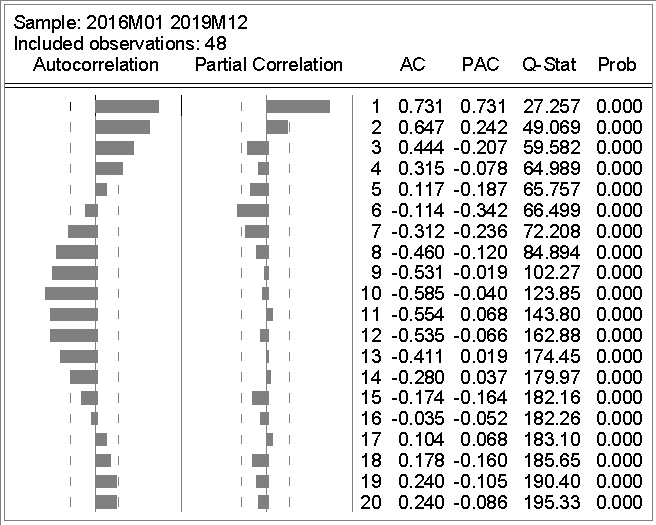
\includegraphics[]{annexe/3_1_extra_cor_ble19.pdf}
    \caption{Corrélograme des résidus des MCO de l'échantillon 2016-2019 du blé}
\end{figure}

\begin{figure}[H]
    \centering
    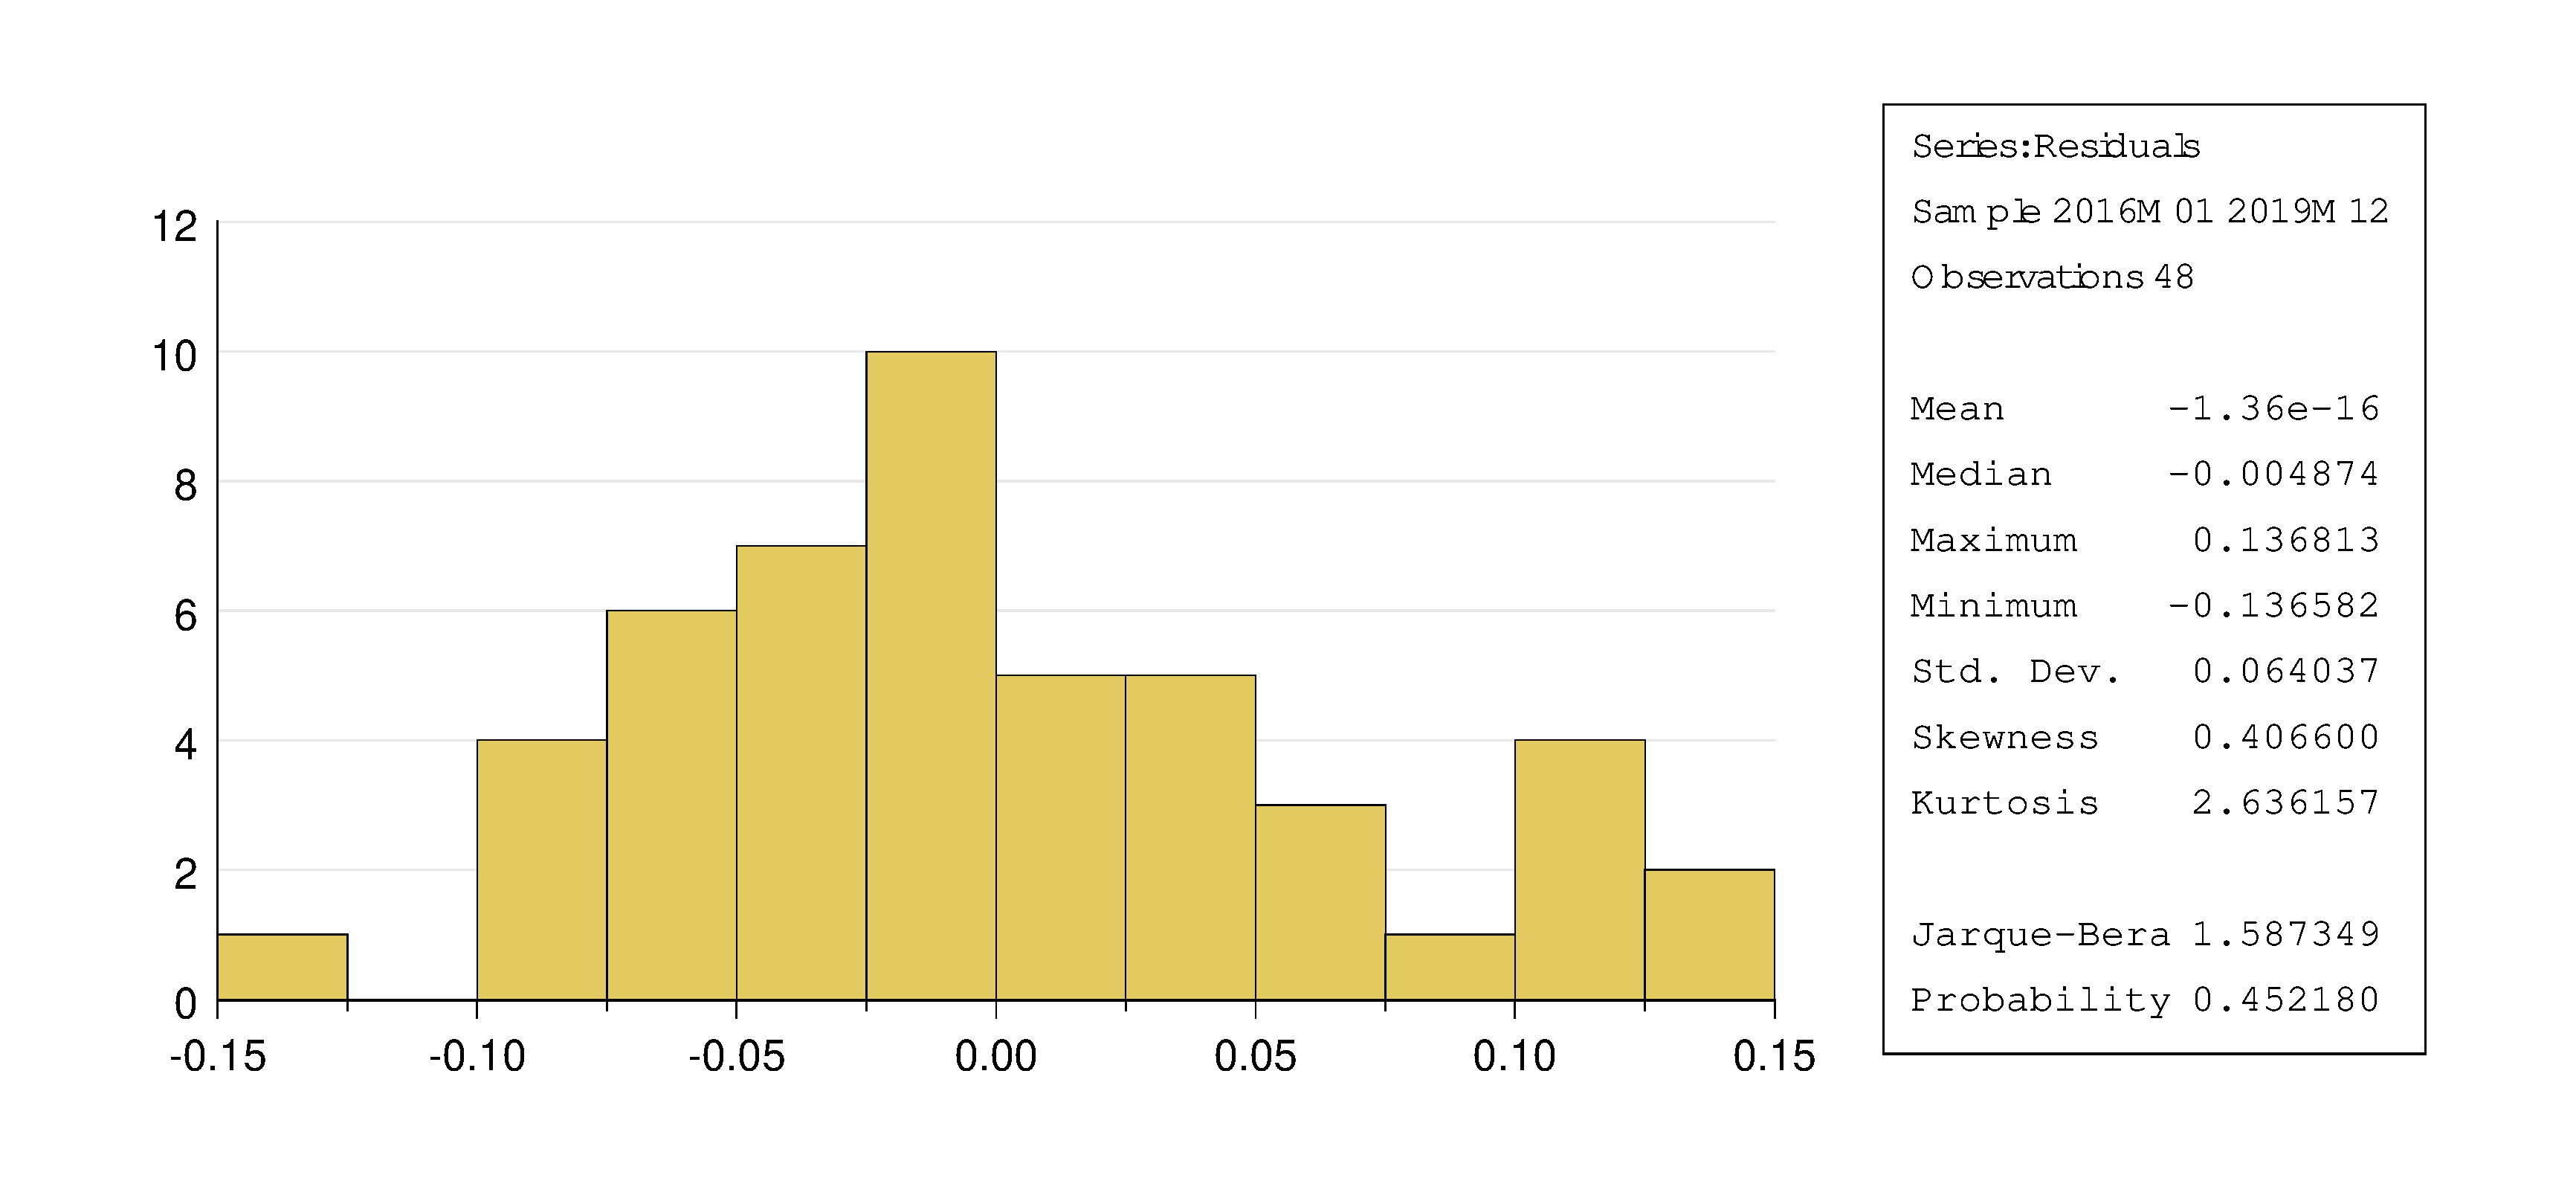
\includegraphics[width=\textwidth]{annexe/3_1_extra_hist_ble19.eps}
    \caption{Histogramme des résidus des MCO de l'échantillon 2016-2019 du blé}
    \label{fig:extra_hist_ble19}
\end{figure}

\begin{table}[H]
    \centering
    \caption{Test ARCH sur les résidus des MCO de l'échantillon 2016-2019 du blé}
    \sffamily
    \begin{tabular}{lrrrr}
\toprule
\multicolumn{2}{l}{Heteroskedasticity Test: ARCH}&\multicolumn{1}{c}{}&\multicolumn{1}{c}{}&\multicolumn{1}{c}{}\\
 \midrule 
\multicolumn{1}{l}{F-statistic}&\multicolumn{1}{r}{3.103962}&\multicolumn{2}{l}{Prob. F(7,33)}&\multicolumn{1}{r}{0.0125}\\
\multicolumn{1}{l}{Obs*R-squared}&\multicolumn{1}{r}{16.27762}&\multicolumn{2}{l}{Prob. Chi-Square(7)}&\multicolumn{1}{r}{0.0227}\\
 \midrule 
\multicolumn{1}{l}{Test Equation:}&\multicolumn{1}{c}{}&\multicolumn{1}{c}{}&\multicolumn{1}{c}{}&\multicolumn{1}{c}{}\\
\multicolumn{2}{l}{Dependent Variable: RESID\textasciicircum 2}&\multicolumn{1}{c}{}&\multicolumn{1}{c}{}&\multicolumn{1}{c}{}\\
\multicolumn{2}{l}{Method: Least Squares}&\multicolumn{1}{c}{}&\multicolumn{1}{c}{}&\multicolumn{1}{c}{}\\
\multicolumn{3}{l}{Sample (adjusted): 2016M08 2019M12}&\multicolumn{1}{c}{}&\multicolumn{1}{c}{}\\
\multicolumn{4}{l}{Included observations: 41 after adjustments}&\multicolumn{1}{c}{}\\
 \bottomrule 
\end{tabular}

    \label{tab:extra_arch_ble19}
\end{table}

\subsubsection{Lissage exponentiel double}
\begin{table}[H]
    \centering
    \caption{Constante de lissage LED blé (2016-2019)}
    \sffamily
    \begin{tabular}{lrrrr}
\toprule
\multicolumn{3}{l}{Sample: 2016M01 2019M12}&\multicolumn{1}{c}{}&\multicolumn{1}{c}{}\\
\multicolumn{3}{l}{Included observations: 48}&\multicolumn{1}{c}{}&\multicolumn{1}{c}{}\\
\multicolumn{3}{l}{Method: Double Exponential}&\multicolumn{1}{c}{}&\multicolumn{1}{c}{}\\
\multicolumn{3}{l}{Original Series: LBLE\_19}&\multicolumn{1}{c}{}&\multicolumn{1}{c}{}\\
\multicolumn{3}{l}{Forecast Series: LBLE\_19\_LED}&\multicolumn{1}{c}{}&\multicolumn{1}{c}{}\\
\midrule
\multicolumn{1}{l}{Parameters:}&\multicolumn{1}{l}{Alpha}&\multicolumn{1}{c}{}&\multicolumn{1}{c}{}&\multicolumn{1}{r}{0.4280}\\
\multicolumn{3}{l}{Sum of Squared Residuals}&\multicolumn{1}{c}{}&\multicolumn{1}{r}{0.104149}\\
\multicolumn{3}{l}{Root Mean Squared Error}&\multicolumn{1}{c}{}&\multicolumn{1}{r}{0.046581}\\
\bottomrule
\end{tabular}
    \label{tab:led_ble19}
\end{table}

\begin{table}[H]
    \centering
    \caption{Constante de lissage LED nickel (2016-2019)}
    \sffamily
    
\begin{tabular}{lrrrr}
\toprule
\multicolumn{3}{l}{Sample: 2016M01 2019M12}&\multicolumn{1}{c}{}&\multicolumn{1}{c}{}\\
\multicolumn{3}{l}{Included observations: 48}&\multicolumn{1}{c}{}&\multicolumn{1}{c}{}\\
\multicolumn{3}{l}{Method: Double Exponential}&\multicolumn{1}{c}{}&\multicolumn{1}{c}{}\\
\multicolumn{3}{l}{Original Series: LNICKEL\_19}&\multicolumn{1}{c}{}&\multicolumn{1}{c}{}\\
\multicolumn{4}{l}{Forecast Series: LNICKEL\_19\_LED}&\multicolumn{1}{c}{}\\
\midrule
\multicolumn{1}{l}{Parameters:}&\multicolumn{1}{l}{Alpha}&\multicolumn{1}{c}{}&\multicolumn{1}{c}{}&\multicolumn{1}{r}{0.4700}\\
\multicolumn{3}{l}{Sum of Squared Residuals}&\multicolumn{1}{c}{}&\multicolumn{1}{r}{0.467077}\\
\multicolumn{3}{l}{Root Mean Squared Error}&\multicolumn{1}{c}{}&\multicolumn{1}{r}{0.098645}\\
\bottomrule
\end{tabular}

    \label{tab:led_nickel19}
\end{table}

\subsubsection{Lissage exponentiel de Holt-Winter}
\begin{table}[H]
    \centering
    \caption{Constantes de lissage HW blé (2016-2019)}
    \sffamily
    
\begin{tabular}{lrrrr}
\toprule
\multicolumn{3}{l}{Sample: 2016M01 2019M12}&\multicolumn{1}{c}{}&\multicolumn{1}{c}{}\\
\multicolumn{3}{l}{Included observations: 48}&\multicolumn{1}{c}{}&\multicolumn{1}{c}{}\\
\multicolumn{4}{l}{Method: Holt-Winters No Seasonal}&\multicolumn{1}{c}{}\\
\multicolumn{3}{l}{Original Series: LBLE\_19}&\multicolumn{1}{c}{}&\multicolumn{1}{c}{}\\
\multicolumn{3}{l}{Forecast Series: LBLE\_19\_HW}&\multicolumn{1}{c}{}&\multicolumn{1}{c}{}\\
\midrule
\multicolumn{1}{l}{Parameters:}&\multicolumn{1}{l}{Alpha}&\multicolumn{1}{c}{}&\multicolumn{1}{c}{}&\multicolumn{1}{r}{0.7800}\\
\multicolumn{1}{c}{}&\multicolumn{1}{l}{Beta}&\multicolumn{1}{c}{}&\multicolumn{1}{c}{}&\multicolumn{1}{r}{0.0000}\\
\multicolumn{3}{l}{Sum of Squared Residuals}&\multicolumn{1}{c}{}&\multicolumn{1}{r}{0.095621}\\
\multicolumn{3}{l}{Root Mean Squared Error}&\multicolumn{1}{c}{}&\multicolumn{1}{r}{0.044633}\\
\bottomrule
\end{tabular}

    \label{tab:hwout_ble19}
\end{table}
\begin{table}[H]
    \centering
    \caption{Constantes de lissage HW nickel (2016-2019)}
    \sffamily
    \begin{tabular}{lrrrr}
\toprule
\multicolumn{3}{l}{Sample: 2016M01 2019M12}&\multicolumn{1}{c}{}&\multicolumn{1}{c}{}\\
\multicolumn{3}{l}{Included observations: 48}&\multicolumn{1}{c}{}&\multicolumn{1}{c}{}\\
\multicolumn{4}{l}{Method: Holt-Winters No Seasonal}&\multicolumn{1}{c}{}\\
\multicolumn{3}{l}{Original Series: LNICKEL\_19}&\multicolumn{1}{c}{}&\multicolumn{1}{c}{}\\
\multicolumn{4}{l}{Forecast Series: LNICKEL\_19\_HW}&\multicolumn{1}{c}{}\\
\midrule
\multicolumn{1}{l}{Parameters:}&\multicolumn{1}{l}{Alpha}&\multicolumn{1}{c}{}&\multicolumn{1}{c}{}&\multicolumn{1}{r}{0.8900}\\
\multicolumn{1}{c}{}&\multicolumn{1}{l}{Beta}&\multicolumn{1}{c}{}&\multicolumn{1}{c}{}&\multicolumn{1}{r}{0.0000}\\
\multicolumn{3}{l}{Sum of Squared Residuals}&\multicolumn{1}{c}{}&\multicolumn{1}{r}{0.378752}\\
\multicolumn{3}{l}{Root Mean Squared Error}&\multicolumn{1}{c}{}&\multicolumn{1}{r}{0.088829}\\
\bottomrule
\end{tabular}


    \label{tab:hwout_nickel19}
\end{table}


\subsection{Échantillon 2016-2021}
\subsubsection{Extrapolation d'une droite de tendance}
\begin{table}[H]
    \centering
    \caption{Estimation par les MCO de l'échantillon 2016-2021 du blé}
    \sffamily
    \label{tab:mco_ble21}
    \begin{tabular}{lrrrr}
\toprule
\multicolumn{2}{l}{Dependent Variable: LBLE\_21}&\multicolumn{1}{c}{}&\multicolumn{1}{c}{}&\multicolumn{1}{c}{}\\
\multicolumn{2}{l}{Method: Least Squares}&\multicolumn{1}{c}{}&\multicolumn{1}{c}{}&\multicolumn{1}{c}{}\\
\multicolumn{2}{l}{Sample: 2016M01 2021M12}&\multicolumn{1}{c}{}&\multicolumn{1}{c}{}&\multicolumn{1}{c}{}\\
\multicolumn{2}{l}{Included observations: 72}&\multicolumn{1}{c}{}&\multicolumn{1}{c}{}&\multicolumn{1}{c}{}\\
\midrule
\multicolumn{1}{c}{Variable}&\multicolumn{1}{r}{Coefficient}&\multicolumn{1}{r}{Std. Error}&\multicolumn{1}{r}{t-Statistic}&\multicolumn{1}{r}{Prob.}\\
\midrule
\multicolumn{1}{c}{@TREND}&\multicolumn{1}{r}{0.006244}&\multicolumn{1}{r}{0.000471}&\multicolumn{1}{r}{13.24514}&\multicolumn{1}{r}{0.0000}\\
\multicolumn{1}{c}{C}&\multicolumn{1}{r}{5.007174}&\multicolumn{1}{r}{0.019392}&\multicolumn{1}{r}{258.2090}&\multicolumn{1}{r}{0.0000}\\
\midrule
\multicolumn{1}{l}{R-squared}&\multicolumn{1}{r}{0.714791}&\multicolumn{2}{l}{Mean dependent var}&\multicolumn{1}{r}{5.228833}\\
\multicolumn{1}{l}{Adjusted R-squared}&\multicolumn{1}{r}{0.710716}&\multicolumn{2}{l}{S.D. dependent var}&\multicolumn{1}{r}{0.154562}\\
\multicolumn{1}{l}{S.E. of regression}&\multicolumn{1}{r}{0.083132}&\multicolumn{2}{l}{Akaike info criterion}&\multicolumn{1}{r}{-2.109399}\\
\multicolumn{1}{l}{Sum squared resid}&\multicolumn{1}{r}{0.483760}&\multicolumn{2}{l}{Schwarz criterion}&\multicolumn{1}{r}{-2.046159}\\
\multicolumn{1}{l}{Log likelihood}&\multicolumn{1}{r}{77.93838}&\multicolumn{2}{l}{Hannan-Quinn criter.}&\multicolumn{1}{r}{-2.084223}\\
\multicolumn{1}{l}{F-statistic}&\multicolumn{1}{r}{175.4338}&\multicolumn{2}{l}{Durbin-Watson stat}&\multicolumn{1}{r}{0.473428}\\
\multicolumn{1}{l}{Prob(F-statistic)}&\multicolumn{1}{r}{0.000000}&\multicolumn{1}{c}{}&\multicolumn{1}{c}{}&\multicolumn{1}{c}{}\\
\bottomrule
\end{tabular}

\end{table}

\begin{figure}[H]
    \centering
    \label{fig:mco_cor_ble21}
    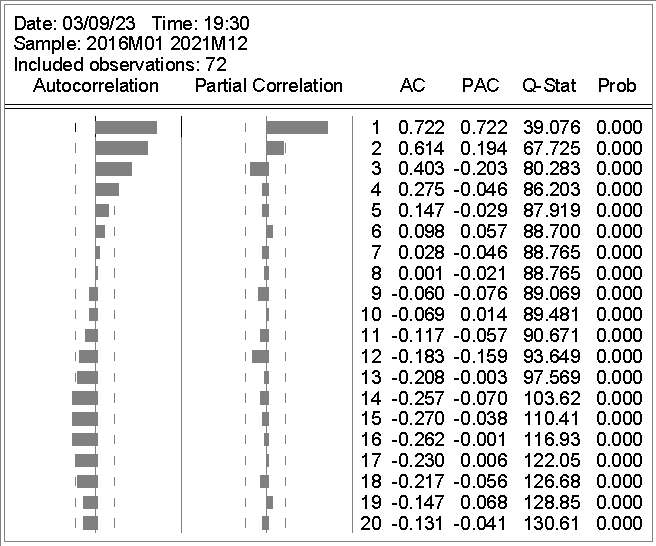
\includegraphics[]{annexe/3_2_mco_corr_ble.pdf}
    \caption{Corrélograme des résidus des MCO de l'échantillon 2016-2021 du blé}
\end{figure}

\begin{figure}[H]
    \centering
    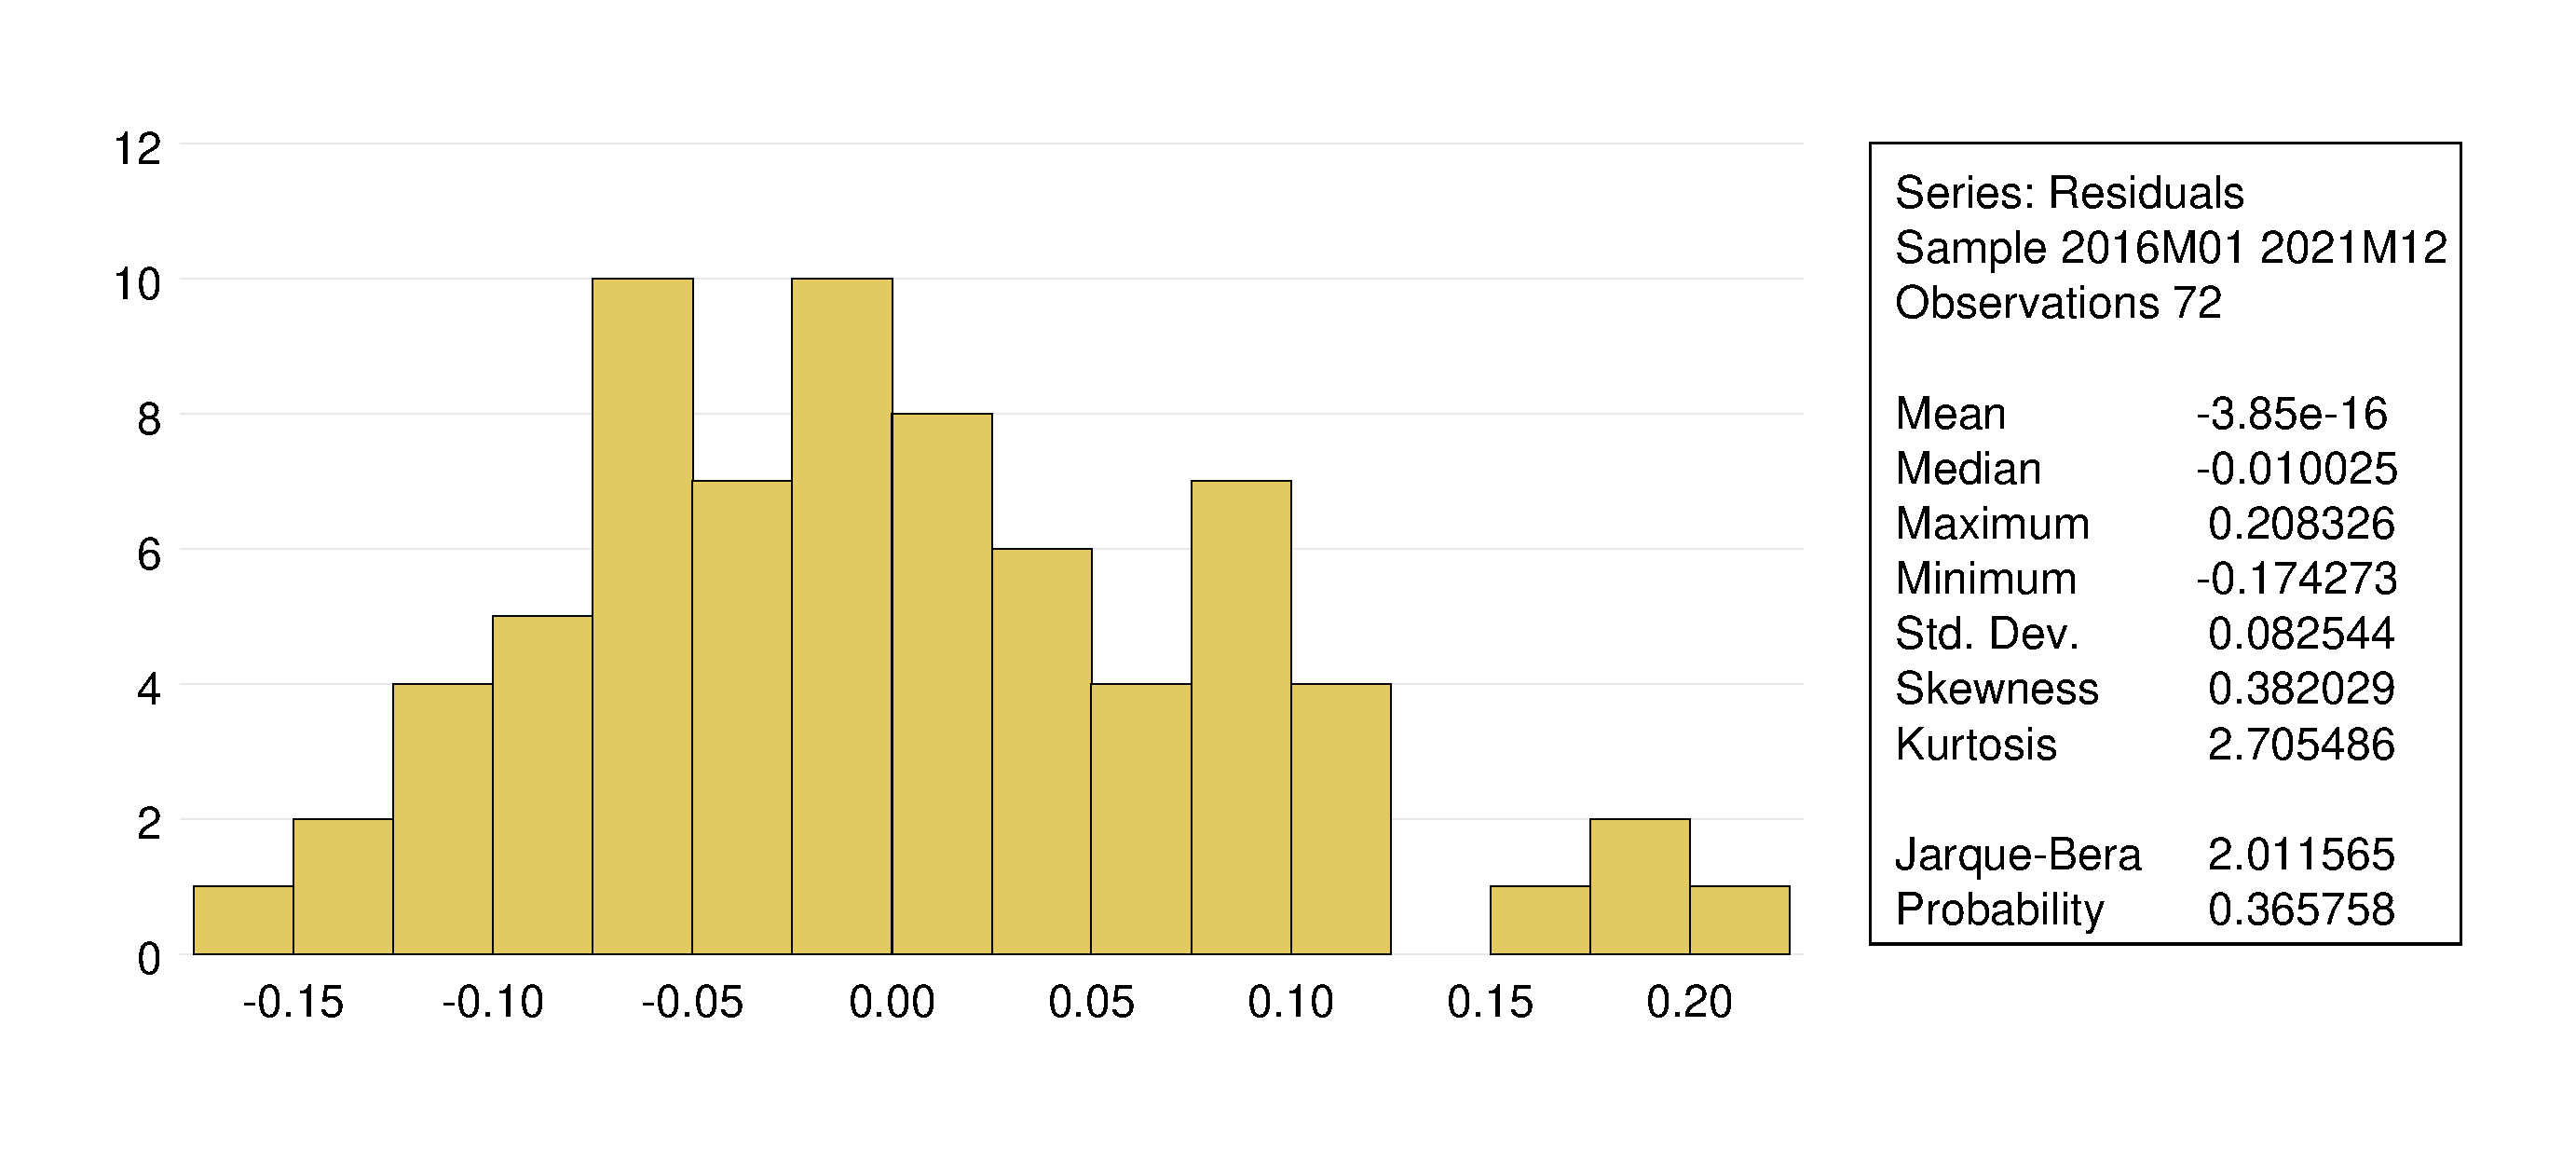
\includegraphics[width=\textwidth]{annexe/3_2_mco_hist_ble.eps}
    \caption{Histogramme des résidus des MCO de l'échantillon 2016-2021 du blé}
    \label{fig:mco_hist_ble21}
\end{figure}

\begin{table}[H]
    \centering
    \caption{Test ARCH sur les résidus des MCO de l'échantillon 2016-2021 du blé}
    \sffamily
    \begin{tabular}{lrrrr}
\toprule
\multicolumn{2}{l}{Heteroskedasticity Test: ARCH}&\multicolumn{1}{c}{}&\multicolumn{1}{c}{}&\multicolumn{1}{c}{}\\
\midrule
\multicolumn{1}{l}{F-statistic}&\multicolumn{1}{r}{8.190606}&\multicolumn{2}{l}{Prob. F(7,57)}&\multicolumn{1}{r}{0.0000}\\
\multicolumn{1}{l}{Obs*R-squared}&\multicolumn{1}{r}{32.59501}&\multicolumn{2}{l}{Prob. Chi-Square(7)}&\multicolumn{1}{r}{0.0000}\\
\midrule
\multicolumn{1}{l}{Test Equation:}&\multicolumn{1}{c}{}&\multicolumn{1}{c}{}&\multicolumn{1}{c}{}&\multicolumn{1}{c}{}\\
\multicolumn{2}{l}{Dependent Variable: RESID\textasciicircum 2}&\multicolumn{1}{c}{}&\multicolumn{1}{c}{}&\multicolumn{1}{c}{}\\
\multicolumn{2}{l}{Method: Least Squares}&\multicolumn{1}{c}{}&\multicolumn{1}{c}{}&\multicolumn{1}{c}{}\\
\multicolumn{3}{l}{Sample (adjusted): 2016M08 2021M12}&\multicolumn{1}{c}{}&\multicolumn{1}{c}{}\\
\multicolumn{4}{l}{Included observations: 65 after adjustments}&\multicolumn{1}{c}{}\\
\bottomrule
\end{tabular}


    \label{tab:mco_homo_ble19}
\end{table}

\begin{table}[H]
    \centering
    \caption{Estimation par les MCO de l'échantillon 2016-2021 du nickel}
    \sffamily
    \label{tab:mco_nickel21}
    \begin{tabular}{lrrrr}
\toprule
\multicolumn{3}{l}{Dependent Variable: SLNICKEL\_21}&\multicolumn{1}{c}{}&\multicolumn{1}{c}{}\\
\multicolumn{2}{l}{Method: Least Squares}&\multicolumn{1}{c}{}&\multicolumn{1}{c}{}&\multicolumn{1}{c}{}\\
\multicolumn{2}{l}{Sample: 2016M01 2021M12}&\multicolumn{1}{c}{}&\multicolumn{1}{c}{}&\multicolumn{1}{c}{}\\
\multicolumn{2}{l}{Included observations: 72}&\multicolumn{1}{c}{}&\multicolumn{1}{c}{}&\multicolumn{1}{c}{}\\
\midrule
\multicolumn{1}{c}{Variable}&\multicolumn{1}{r}{Coefficient}&\multicolumn{1}{r}{Std. Error}&\multicolumn{1}{r}{t-Statistic}&\multicolumn{1}{r}{Prob.}\\
\midrule
\multicolumn{1}{c}{@TREND}&\multicolumn{1}{r}{0.009946}&\multicolumn{1}{r}{0.000625}&\multicolumn{1}{r}{15.91309}&\multicolumn{1}{r}{0.0000}\\
\multicolumn{1}{c}{C}&\multicolumn{1}{r}{9.114432}&\multicolumn{1}{r}{0.025711}&\multicolumn{1}{r}{354.5001}&\multicolumn{1}{r}{0.0000}\\
\midrule
\multicolumn{1}{l}{R-squared}&\multicolumn{1}{r}{0.783434}&\multicolumn{2}{l}{Mean dependent var}&\multicolumn{1}{r}{9.467514}\\
\multicolumn{1}{l}{Adjusted R-squared}&\multicolumn{1}{r}{0.780340}&\multicolumn{2}{l}{S.D. dependent var}&\multicolumn{1}{r}{0.235170}\\
\multicolumn{1}{l}{S.E. of regression}&\multicolumn{1}{r}{0.110219}&\multicolumn{2}{l}{Akaike info criterion}&\multicolumn{1}{r}{-1.545304}\\
\multicolumn{1}{l}{Sum squared resid}&\multicolumn{1}{r}{0.850382}&\multicolumn{2}{l}{Schwarz criterion}&\multicolumn{1}{r}{-1.482063}\\
\multicolumn{1}{l}{Log likelihood}&\multicolumn{1}{r}{57.63093}&\multicolumn{2}{l}{Hannan-Quinn criter.}&\multicolumn{1}{r}{-1.520127}\\
\multicolumn{1}{l}{F-statistic}&\multicolumn{1}{r}{253.2265}&\multicolumn{2}{l}{Durbin-Watson stat}&\multicolumn{1}{r}{0.466778}\\
\multicolumn{1}{l}{Prob(F-statistic)}&\multicolumn{1}{r}{0.000000}&\multicolumn{1}{c}{}&\multicolumn{1}{c}{}&\multicolumn{1}{c}{}\\
\bottomrule
\end{tabular}

\end{table}

\begin{figure}[H]
    \centering
    \label{fig:mco_cor_nickel21}
    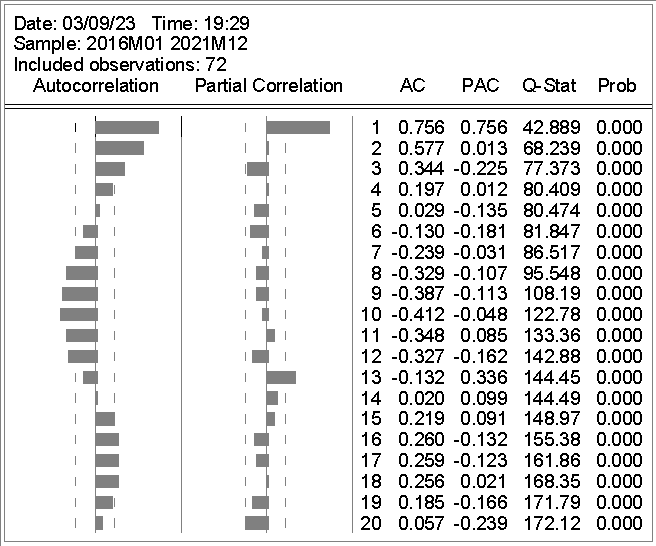
\includegraphics[]{annexe/3_2_mco_corr_nickel.pdf}
    \caption{Corrélograme des résidus des MCO de l'échantillon 2016-2021 du nickel}
\end{figure}

\begin{figure}[H]
    \centering
    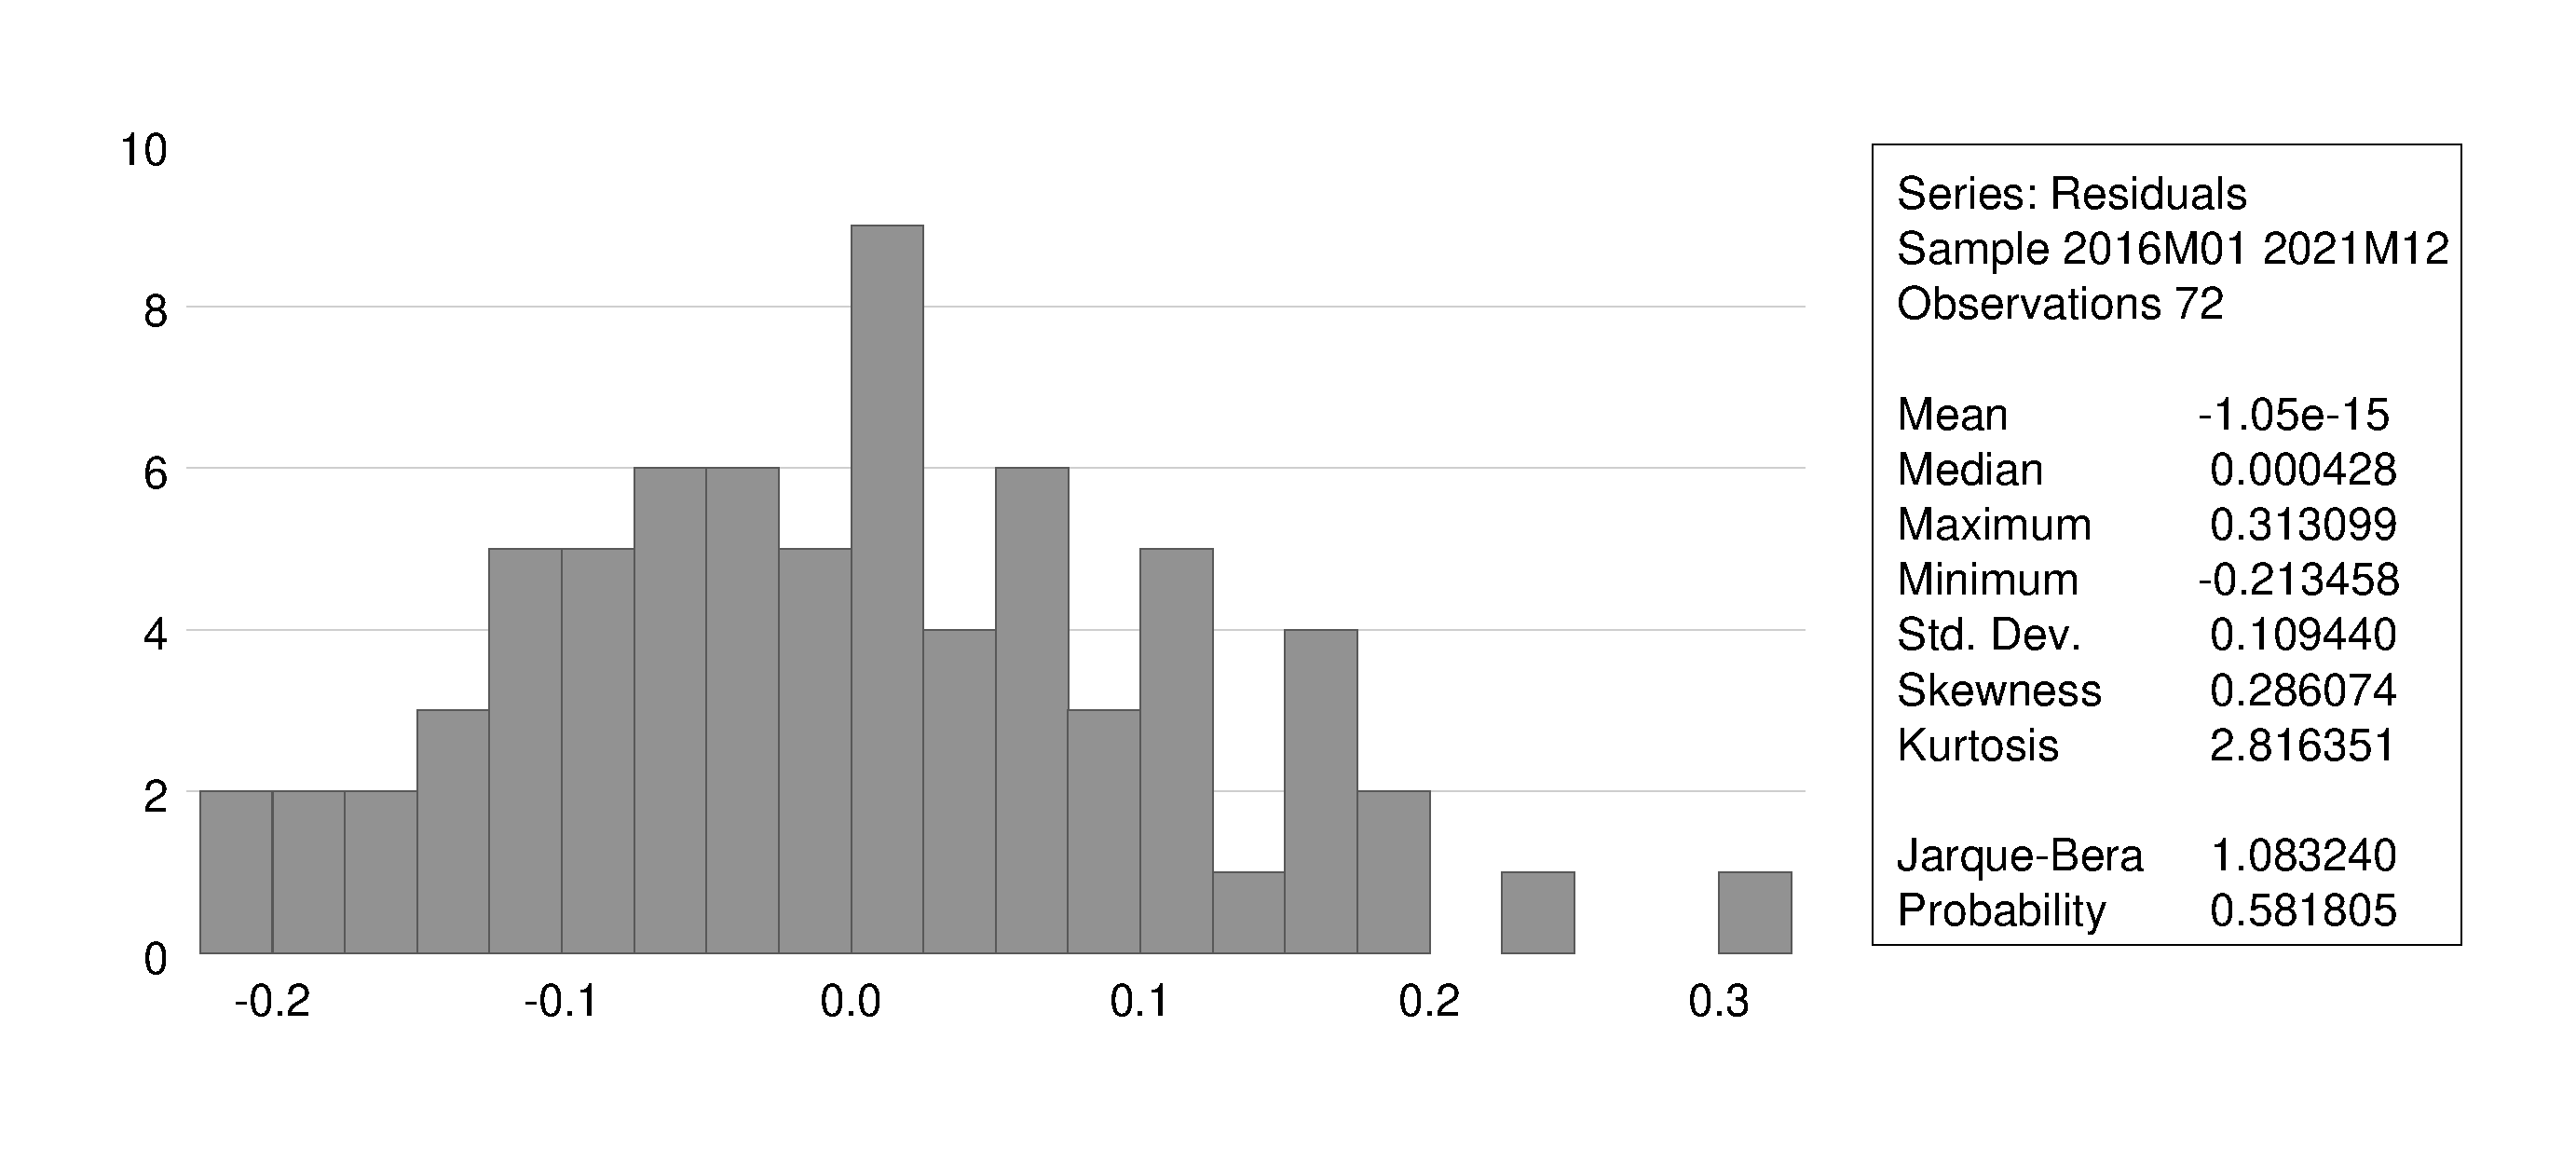
\includegraphics[width=\textwidth]{annexe/3_2_mco_hist_nickel.eps}
    \caption{Histogramme des résidus des MCO de l'échantillon 2016-2021 du nickel}
    \label{fig:mco_hist_nickel21}
\end{figure}

\begin{table}[H]
    \centering
    \caption{Test ARCH sur les résidus des MCO de l'échantillon 2016-2021 du nickel}
    \sffamily
    \begin{tabular}{lrrrr}
\toprule
\multicolumn{2}{l}{Heteroskedasticity Test: ARCH}&\multicolumn{1}{c}{}&\multicolumn{1}{c}{}&\multicolumn{1}{c}{}\\
\midrule
\multicolumn{1}{l}{F-statistic}&\multicolumn{1}{r}{4.383482}&\multicolumn{2}{l}{Prob. F(7,57)}&\multicolumn{1}{r}{0.0006}\\
\multicolumn{1}{l}{Obs*R-squared}&\multicolumn{1}{r}{22.74618}&\multicolumn{2}{l}{Prob. Chi-Square(7)}&\multicolumn{1}{r}{0.0019}\\
\midrule
\multicolumn{1}{l}{Test Equation:}&\multicolumn{1}{c}{}&\multicolumn{1}{c}{}&\multicolumn{1}{c}{}&\multicolumn{1}{c}{}\\
\multicolumn{2}{l}{Dependent Variable: RESID\textasciicircum 2}&\multicolumn{1}{c}{}&\multicolumn{1}{c}{}&\multicolumn{1}{c}{}\\
\multicolumn{2}{l}{Method: Least Squares}&\multicolumn{1}{c}{}&\multicolumn{1}{c}{}&\multicolumn{1}{c}{}\\
\multicolumn{3}{l}{Sample (adjusted): 2016M08 2021M12}&\multicolumn{1}{c}{}&\multicolumn{1}{c}{}\\
\multicolumn{4}{l}{Included observations: 65 after adjustments}&\multicolumn{1}{c}{}\\
\bottomrule
\end{tabular}

    \label{tab:mco_homo_nickel19}
\end{table}

\subsubsection{Lissage exponentiel double}
\begin{table}[H]
    \centering
    \caption{Constante de lissage LED blé (2016-2021)}
    \sffamily
    \begin{tabular}{lrrrr}
\toprule
\multicolumn{3}{l}{Sample: 2016M01 2021M12}&\multicolumn{1}{c}{}&\multicolumn{1}{c}{}\\
\multicolumn{3}{l}{Included observations: 72}&\multicolumn{1}{c}{}&\multicolumn{1}{c}{}\\
\multicolumn{3}{l}{Method: Double Exponential}&\multicolumn{1}{c}{}&\multicolumn{1}{c}{}\\
\multicolumn{3}{l}{Original Series: LBLE\_21}&\multicolumn{1}{c}{}&\multicolumn{1}{c}{}\\
\multicolumn{3}{l}{Forecast Series: LBLE\_21\_LED}&\multicolumn{1}{c}{}&\multicolumn{1}{c}{}\\
\midrule
\multicolumn{1}{l}{Parameters:}&\multicolumn{1}{l}{Alpha}&\multicolumn{1}{c}{}&\multicolumn{1}{c}{}&\multicolumn{1}{r}{0.3720}\\
\multicolumn{3}{l}{Sum of Squared Residuals}&\multicolumn{1}{c}{}&\multicolumn{1}{r}{0.236817}\\
\multicolumn{3}{l}{Root Mean Squared Error}&\multicolumn{1}{c}{}&\multicolumn{1}{r}{0.057351}\\
\bottomrule
\end{tabular}
    \label{tab:led_ble21}
\end{table}

\begin{table}[H]
    \centering
    \caption{Constante de lissage LED nickel (2016-2021)}
    \sffamily
    \begin{tabular}{lrrrr}
\toprule
\multicolumn{3}{l}{Sample: 2016M01 2021M12}&\multicolumn{1}{c}{}&\multicolumn{1}{c}{}\\
\multicolumn{3}{l}{Included observations: 72}&\multicolumn{1}{c}{}&\multicolumn{1}{c}{}\\
\multicolumn{3}{l}{Method: Double Exponential}&\multicolumn{1}{c}{}&\multicolumn{1}{c}{}\\
\multicolumn{3}{l}{Original Series: SLNICKEL\_21}&\multicolumn{1}{c}{}&\multicolumn{1}{c}{}\\
\multicolumn{4}{l}{Forecast Series: SLNICKEL\_21\_LED}&\multicolumn{1}{c}{}\\
\midrule
\multicolumn{1}{l}{Parameters:}&\multicolumn{1}{l}{Alpha}&\multicolumn{1}{c}{}&\multicolumn{1}{c}{}&\multicolumn{1}{r}{0.5040}\\
\multicolumn{3}{l}{Sum of Squared Residuals}&\multicolumn{1}{c}{}&\multicolumn{1}{r}{0.472073}\\
\multicolumn{3}{l}{Root Mean Squared Error}&\multicolumn{1}{c}{}&\multicolumn{1}{r}{0.080973}\\
\midrule
\multicolumn{2}{l}{End of Period Levels:}&\multicolumn{1}{l}{Mean}&\multicolumn{1}{c}{}&\multicolumn{1}{r}{9.932757}\\
\multicolumn{1}{c}{}&\multicolumn{1}{c}{}&\multicolumn{1}{l}{Trend}&\multicolumn{1}{c}{}&\multicolumn{1}{r}{0.031719}\\
\bottomrule
\end{tabular}


    \label{tab:led_nickel21}
\end{table}

\subsubsection{Lissage exponentiel de Holt-Winter}
\begin{table}[H]
    \centering
    \caption{Constantes de lissage HW blé (2016-2021)}
    \sffamily
    \begin{tabular}{lrrrr}
\toprule
\multicolumn{3}{l}{Sample: 2016M01 2021M12}&\multicolumn{1}{c}{}&\multicolumn{1}{c}{}\\
\multicolumn{3}{l}{Included observations: 72}&\multicolumn{1}{c}{}&\multicolumn{1}{c}{}\\
\multicolumn{4}{l}{Method: Holt-Winters No Seasonal}&\multicolumn{1}{c}{}\\
\multicolumn{3}{l}{Original Series: LBLE\_21}&\multicolumn{1}{c}{}&\multicolumn{1}{c}{}\\
\multicolumn{3}{l}{Forecast Series: LBLE\_21\_HW}&\multicolumn{1}{c}{}&\multicolumn{1}{c}{}\\
\midrule
\multicolumn{1}{l}{Parameters:}&\multicolumn{1}{l}{Alpha}&\multicolumn{1}{c}{}&\multicolumn{1}{c}{}&\multicolumn{1}{r}{0.7300}\\
\multicolumn{1}{c}{}&\multicolumn{1}{l}{Beta}&\multicolumn{1}{c}{}&\multicolumn{1}{c}{}&\multicolumn{1}{r}{0.0000}\\
\multicolumn{3}{l}{Sum of Squared Residuals}&\multicolumn{1}{c}{}&\multicolumn{1}{r}{0.209799}\\
\multicolumn{3}{l}{Root Mean Squared Error}&\multicolumn{1}{c}{}&\multicolumn{1}{r}{0.053980}\\
\bottomrule
\end{tabular}

    \label{tab:hw_ble}
\end{table}
\begin{table}[H]
    \centering
    \caption{Constantes de lissage HW nickel (2016-2021)}
    \sffamily
    \begin{tabular}{lrrrr}
\toprule
\multicolumn{3}{l}{Sample: 2016M01 2021M12}&\multicolumn{1}{c}{}&\multicolumn{1}{c}{}\\
\multicolumn{3}{l}{Included observations: 72}&\multicolumn{1}{c}{}&\multicolumn{1}{c}{}\\
\multicolumn{4}{l}{Method: Holt-Winters Additive Seasonal}&\multicolumn{1}{c}{}\\
\multicolumn{3}{l}{Original Series: LNICKEL\_21}&\multicolumn{1}{c}{}&\multicolumn{1}{c}{}\\
\multicolumn{4}{l}{Forecast Series: LNICKEL\_21\_HW}&\multicolumn{1}{c}{}\\
\midrule
\multicolumn{1}{l}{Parameters:}&\multicolumn{1}{l}{Alpha}&\multicolumn{1}{c}{}&\multicolumn{1}{c}{}&\multicolumn{1}{r}{0.9000}\\
\multicolumn{1}{c}{}&\multicolumn{1}{l}{Beta}&\multicolumn{1}{c}{}&\multicolumn{1}{c}{}&\multicolumn{1}{r}{0.0000}\\
\multicolumn{1}{c}{}&\multicolumn{1}{l}{Gamma}&\multicolumn{1}{c}{}&\multicolumn{1}{c}{}&\multicolumn{1}{r}{0.0000}\\
\multicolumn{3}{l}{Sum of Squared Residuals}&\multicolumn{1}{c}{}&\multicolumn{1}{r}{0.381191}\\
\multicolumn{3}{l}{Root Mean Squared Error}&\multicolumn{1}{c}{}&\multicolumn{1}{r}{0.072762}\\
\bottomrule
\end{tabular}
    \label{tab:hw_nickel}
\end{table}

\section{Prévision selon la méthodologie de Box-Jenkins}
\setcounter{table}{0}
\setcounter{figure}{0}
\subsection{Test de racine unitaire}
\subsubsection{Echnatillon 2016-2019}
\subsubsection*{Blé}
\begin{table}[H]
    \centering
    \caption{Estimation du modèle 3 pour le blé (2016-2019)}
    \sffamily
    \begin{tabular}{lrrrr}
\toprule
\multicolumn{3}{l}{Null Hypothesis: LBLE\_19 has a unit root}&\multicolumn{1}{c}{}&\multicolumn{1}{c}{}\\
\multicolumn{3}{l}{Exogenous: Constant, Linear Trend}&\multicolumn{1}{c}{}&\multicolumn{1}{c}{}\\
\multicolumn{5}{l}{Bandwidth: 2 (Newey-West automatic) using Bartlett kernel}\\
\midrule
\multicolumn{1}{c}{}&\multicolumn{1}{c}{}&\multicolumn{1}{c}{}&\multicolumn{1}{c}{Adj. t-Stat}&\multicolumn{1}{c}{Prob.*}\\
\midrule
\multicolumn{2}{l}{Phillips-Perron test statistic}&\multicolumn{1}{l}{}&\multicolumn{1}{c}{-2.671980}&\multicolumn{1}{c}{0.2524}\\
\multicolumn{1}{l}{Test critical values:}&\multicolumn{1}{c}{1\% level}&\multicolumn{1}{c}{}&\multicolumn{1}{c}{-4.165756}&\multicolumn{1}{c}{}\\
\multicolumn{1}{c}{}&\multicolumn{1}{c}{5\% level}&\multicolumn{1}{c}{}&\multicolumn{1}{c}{-3.508508}&\multicolumn{1}{c}{}\\
\multicolumn{1}{c}{}&\multicolumn{1}{c}{10\% level}&\multicolumn{1}{c}{}&\multicolumn{1}{c}{-3.184230}&\multicolumn{1}{c}{}\\
\midrule
\multicolumn{2}{l}{Phillips-Perron Test Equation}&\multicolumn{1}{c}{}&\multicolumn{1}{c}{}&\multicolumn{1}{c}{}\\
\multicolumn{3}{l}{Dependent Variable: D(LBLE\_19)}&\multicolumn{1}{c}{}&\multicolumn{1}{c}{}\\
\multicolumn{2}{l}{Method: Least Squares}&\multicolumn{1}{c}{}&\multicolumn{1}{c}{}&\multicolumn{1}{c}{}\\
\multicolumn{3}{l}{Sample (adjusted): 2016M02 2019M12}&\multicolumn{1}{c}{}&\multicolumn{1}{c}{}\\
\multicolumn{4}{l}{Included observations: 47 after adjustments}&\multicolumn{1}{c}{}\\
\midrule
\multicolumn{1}{c}{Variable}&\multicolumn{1}{r}{Coefficient}&\multicolumn{1}{r}{Std. Error}&\multicolumn{1}{r}{t-Statistic}&\multicolumn{1}{r}{Prob.}\\
\midrule
\multicolumn{1}{c}{LBLE\_19(-1)}&\multicolumn{1}{r}{-0.268617}&\multicolumn{1}{r}{0.101366}&\multicolumn{1}{r}{-2.649965}&\multicolumn{1}{r}{0.0111}\\
\multicolumn{1}{c}{C}&\multicolumn{1}{r}{1.355316}&\multicolumn{1}{r}{0.511357}&\multicolumn{1}{r}{2.650430}&\multicolumn{1}{r}{0.0111}\\
\multicolumn{1}{c}{@TREND("2016M01")}&\multicolumn{1}{r}{0.001295}&\multicolumn{1}{r}{0.000658}&\multicolumn{1}{r}{1.967975}&\multicolumn{1}{r}{0.0554}\\
\midrule
\multicolumn{1}{l}{R-squared}&\multicolumn{1}{r}{0.138331}&\multicolumn{2}{l}{Mean dependent var}&\multicolumn{1}{r}{0.003023}\\
\multicolumn{1}{l}{Adjusted R-squared}&\multicolumn{1}{r}{0.099164}&\multicolumn{2}{l}{S.D. dependent var}&\multicolumn{1}{r}{0.046856}\\
\multicolumn{1}{l}{S.E. of regression}&\multicolumn{1}{r}{0.044473}&\multicolumn{2}{l}{Akaike info criterion}&\multicolumn{1}{r}{-3.326190}\\
\multicolumn{1}{l}{Sum squared resid}&\multicolumn{1}{r}{0.087023}&\multicolumn{2}{l}{Schwarz criterion}&\multicolumn{1}{r}{-3.208095}\\
\multicolumn{1}{l}{Log likelihood}&\multicolumn{1}{r}{81.16545}&\multicolumn{2}{l}{Hannan-Quinn criter.}&\multicolumn{1}{r}{-3.281750}\\
\multicolumn{1}{l}{F-statistic}&\multicolumn{1}{r}{3.531847}&\multicolumn{2}{l}{Durbin-Watson stat}&\multicolumn{1}{r}{2.151360}\\
\multicolumn{1}{l}{Prob(F-statistic)}&\multicolumn{1}{r}{0.037800}&\multicolumn{1}{c}{}&\multicolumn{1}{c}{}&\multicolumn{1}{c}{}\\
\bottomrule
\end{tabular}
    \label{tab:mod3_ble19}
\end{table}

\begin{table}[H]
    \centering
    \caption{Estimation du modèle 3 contraint sous $H_{0}^{3}$ pour le blé (2016-2019)}
    \sffamily
    \begin{tabular}{lrrrr}
\toprule
\multicolumn{3}{l}{Dependent Variable: D(LBLE\_19)}&\multicolumn{1}{c}{}&\multicolumn{1}{c}{}\\
\multicolumn{2}{l}{Method: Least Squares}&\multicolumn{1}{c}{}&\multicolumn{1}{c}{}&\multicolumn{1}{c}{}\\
\multicolumn{3}{l}{Sample (adjusted): 2016M02 2019M12}&\multicolumn{1}{c}{}&\multicolumn{1}{c}{}\\
\multicolumn{4}{l}{Included observations: 47 after adjustments}&\multicolumn{1}{c}{}\\
\midrule
\multicolumn{1}{c}{Variable}&\multicolumn{1}{r}{Coefficient}&\multicolumn{1}{r}{Std. Error}&\multicolumn{1}{r}{t-Statistic}&\multicolumn{1}{r}{Prob.}\\
\midrule
\multicolumn{1}{c}{C}&\multicolumn{1}{r}{0.003023}&\multicolumn{1}{r}{0.006835}&\multicolumn{1}{r}{0.442306}&\multicolumn{1}{r}{0.6603}\\
\midrule
\multicolumn{1}{l}{R-squared}&\multicolumn{1}{r}{0.000000}&\multicolumn{2}{l}{Mean dependent var}&\multicolumn{1}{r}{0.003023}\\
\multicolumn{1}{l}{Adjusted R-squared}&\multicolumn{1}{r}{0.000000}&\multicolumn{2}{l}{S.D. dependent var}&\multicolumn{1}{r}{0.046856}\\
\multicolumn{1}{l}{S.E. of regression}&\multicolumn{1}{r}{0.046856}&\multicolumn{2}{l}{Akaike info criterion}&\multicolumn{1}{r}{-3.262412}\\
\multicolumn{1}{l}{Sum squared resid}&\multicolumn{1}{r}{0.100994}&\multicolumn{2}{l}{Schwarz criterion}&\multicolumn{1}{r}{-3.223047}\\
\multicolumn{1}{l}{Log likelihood}&\multicolumn{1}{r}{77.66668}&\multicolumn{2}{l}{Hannan-Quinn criter.}&\multicolumn{1}{r}{-3.247599}\\
\multicolumn{1}{l}{Durbin-Watson stat}&\multicolumn{1}{r}{2.480204}&\multicolumn{1}{c}{}&\multicolumn{1}{c}{}&\multicolumn{1}{c}{}\\
\bottomrule
\end{tabular}
    \label{tab:mod3cont_ble19}
\end{table}

\begin{table}[H]
    \centering
    \caption{Estimation du modèle 2 pour le blé (2016-2019)}
    \sffamily
    \begin{tabular}{lrrrr}
\toprule
\multicolumn{3}{l}{Null Hypothesis: LBLE\_19 has a unit root}&\multicolumn{1}{c}{}&\multicolumn{1}{c}{}\\
\multicolumn{2}{l}{Exogenous: Constant}&\multicolumn{1}{c}{}&\multicolumn{1}{c}{}&\multicolumn{1}{c}{}\\
\multicolumn{5}{l}{Bandwidth: 0 (Newey-West automatic) using Bartlett kernel}\\
\midrule
\multicolumn{1}{c}{}&\multicolumn{1}{c}{}&\multicolumn{1}{c}{}&\multicolumn{1}{c}{Adj. t-Stat}&\multicolumn{1}{c}{Prob.*}\\
\midrule
\multicolumn{2}{l}{Phillips-Perron test statistic}&\multicolumn{1}{l}{}&\multicolumn{1}{c}{-1.731845}&\multicolumn{1}{c}{0.4090}\\
\multicolumn{1}{l}{Test critical values:}&\multicolumn{1}{c}{1\% level}&\multicolumn{1}{c}{}&\multicolumn{1}{c}{-3.577723}&\multicolumn{1}{c}{}\\
\multicolumn{1}{c}{}&\multicolumn{1}{c}{5\% level}&\multicolumn{1}{c}{}&\multicolumn{1}{c}{-2.925169}&\multicolumn{1}{c}{}\\
\multicolumn{1}{c}{}&\multicolumn{1}{c}{10\% level}&\multicolumn{1}{c}{}&\multicolumn{1}{c}{-2.600658}&\multicolumn{1}{c}{}\\
\midrule
\multicolumn{2}{l}{Phillips-Perron Test Equation}&\multicolumn{1}{c}{}&\multicolumn{1}{c}{}&\multicolumn{1}{c}{}\\
\multicolumn{3}{l}{Dependent Variable: D(LBLE\_19)}&\multicolumn{1}{c}{}&\multicolumn{1}{c}{}\\
\multicolumn{2}{l}{Method: Least Squares}&\multicolumn{1}{c}{}&\multicolumn{1}{c}{}&\multicolumn{1}{c}{}\\
\multicolumn{3}{l}{Sample (adjusted): 2016M02 2019M12}&\multicolumn{1}{c}{}&\multicolumn{1}{c}{}\\
\multicolumn{4}{l}{Included observations: 47 after adjustments}&\multicolumn{1}{c}{}\\
\midrule
\multicolumn{1}{c}{Variable}&\multicolumn{1}{r}{Coefficient}&\multicolumn{1}{r}{Std. Error}&\multicolumn{1}{r}{t-Statistic}&\multicolumn{1}{r}{Prob.}\\
\midrule
\multicolumn{1}{c}{LBLE\_19(-1)}&\multicolumn{1}{r}{-0.131600}&\multicolumn{1}{r}{0.075988}&\multicolumn{1}{r}{-1.731845}&\multicolumn{1}{r}{0.0902}\\
\multicolumn{1}{c}{C}&\multicolumn{1}{r}{0.680760}&\multicolumn{1}{r}{0.391395}&\multicolumn{1}{r}{1.739315}&\multicolumn{1}{r}{0.0888}\\
\midrule
\multicolumn{1}{l}{R-squared}&\multicolumn{1}{r}{0.062486}&\multicolumn{2}{l}{Mean dependent var}&\multicolumn{1}{r}{0.003023}\\
\multicolumn{1}{l}{Adjusted R-squared}&\multicolumn{1}{r}{0.041652}&\multicolumn{2}{l}{S.D. dependent var}&\multicolumn{1}{r}{0.046856}\\
\multicolumn{1}{l}{S.E. of regression}&\multicolumn{1}{r}{0.045870}&\multicolumn{2}{l}{Akaike info criterion}&\multicolumn{1}{r}{-3.284382}\\
\multicolumn{1}{l}{Sum squared resid}&\multicolumn{1}{r}{0.094683}&\multicolumn{2}{l}{Schwarz criterion}&\multicolumn{1}{r}{-3.205653}\\
\multicolumn{1}{l}{Log likelihood}&\multicolumn{1}{r}{79.18298}&\multicolumn{2}{l}{Hannan-Quinn criter.}&\multicolumn{1}{r}{-3.254756}\\
\multicolumn{1}{l}{F-statistic}&\multicolumn{1}{r}{2.999285}&\multicolumn{2}{l}{Durbin-Watson stat}&\multicolumn{1}{r}{2.300599}\\
\multicolumn{1}{l}{Prob(F-statistic)}&\multicolumn{1}{r}{0.090152}&\multicolumn{1}{c}{}&\multicolumn{1}{c}{}&\multicolumn{1}{c}{}\\
\bottomrule
\end{tabular}

    \label{tab:mod2_ble19}
\end{table}

\begin{table}[H]
    \centering
    \caption{Test de nullité de la moyenne du cours du blé (2016-2019)}
    \sffamily
    \begin{tabular}{lrrr}
\toprule
\multicolumn{2}{l}{Hypothesis Testing for LBLE\_19}&\multicolumn{1}{c}{}&\multicolumn{1}{c}{}\\
\multicolumn{3}{l}{Sample (adjusted): 2016M01 2019M12}&\multicolumn{1}{c}{}\\
\multicolumn{3}{l}{Included observations: 48 after adjustments}&\multicolumn{1}{c}{}\\
\multicolumn{3}{l}{Test of Hypothesis: Mean =  0.000000}&\multicolumn{1}{c}{}\\
\midrule
\multicolumn{2}{l}{Sample Mean =  5.151855}&\multicolumn{1}{c}{}&\multicolumn{1}{c}{}\\
\multicolumn{2}{l}{Sample Std. Dev. =  0.089014}&\multicolumn{1}{c}{}&\multicolumn{1}{c}{}\\
\multicolumn{1}{c}{}&\multicolumn{1}{c}{}&\multicolumn{1}{c}{}&\multicolumn{1}{c}{}\\
\multicolumn{1}{l}{Method}&\multicolumn{1}{c}{}&\multicolumn{1}{r}{Value}&\multicolumn{1}{r}{Probability}\\
\multicolumn{1}{l}{t-statistic}&\multicolumn{1}{c}{}&\multicolumn{1}{r}{400.9849}&\multicolumn{1}{r}{0.0000}\\
\bottomrule
\end{tabular}
    \label{tab:testmoy_ble19}
\end{table}

\subsubsection*{Nickel}
\begin{table}[H]
    \centering
    \caption{Estimation du modèle 3 pour le nickel (2016-2019)}
    \sffamily
    \begin{tabular}{lrrrr}
\toprule
\multicolumn{4}{l}{Null Hypothesis: LNICKEL\_19 has a unit root}&\multicolumn{1}{c}{}\\
\multicolumn{3}{l}{Exogenous: Constant, Linear Trend}&\multicolumn{1}{c}{}&\multicolumn{1}{c}{}\\
\multicolumn{5}{l}{Bandwidth: 3 (Newey-West automatic) using Bartlett kernel}\\
\midrule
\multicolumn{1}{c}{}&\multicolumn{1}{c}{}&\multicolumn{1}{c}{}&\multicolumn{1}{c}{Adj. t-Stat}&\multicolumn{1}{c}{Prob.*}\\
\midrule
\multicolumn{2}{l}{Phillips-Perron test statistic}&\multicolumn{1}{l}{}&\multicolumn{1}{c}{-3.039752}&\multicolumn{1}{c}{0.1327}\\
\multicolumn{1}{l}{Test critical values:}&\multicolumn{1}{c}{1\% level}&\multicolumn{1}{c}{}&\multicolumn{1}{c}{-4.165756}&\multicolumn{1}{c}{}\\
\multicolumn{1}{c}{}&\multicolumn{1}{c}{5\% level}&\multicolumn{1}{c}{}&\multicolumn{1}{c}{-3.508508}&\multicolumn{1}{c}{}\\
\multicolumn{1}{c}{}&\multicolumn{1}{c}{10\% level}&\multicolumn{1}{c}{}&\multicolumn{1}{c}{-3.184230}&\multicolumn{1}{c}{}\\
\midrule
\multicolumn{2}{l}{Phillips-Perron Test Equation}&\multicolumn{1}{c}{}&\multicolumn{1}{c}{}&\multicolumn{1}{c}{}\\
\multicolumn{3}{l}{Dependent Variable: D(LNICKEL\_19)}&\multicolumn{1}{c}{}&\multicolumn{1}{c}{}\\
\multicolumn{2}{l}{Method: Least Squares}&\multicolumn{1}{c}{}&\multicolumn{1}{c}{}&\multicolumn{1}{c}{}\\
\multicolumn{3}{l}{Sample (adjusted): 2016M02 2019M12}&\multicolumn{1}{c}{}&\multicolumn{1}{c}{}\\
\multicolumn{4}{l}{Included observations: 47 after adjustments}&\multicolumn{1}{c}{}\\
\midrule
\multicolumn{1}{c}{Variable}&\multicolumn{1}{r}{Coefficient}&\multicolumn{1}{r}{Std. Error}&\multicolumn{1}{r}{t-Statistic}&\multicolumn{1}{r}{Prob.}\\
\midrule
\multicolumn{1}{c}{LNICKEL\_19(-1)}&\multicolumn{1}{r}{-0.336008}&\multicolumn{1}{r}{0.113566}&\multicolumn{1}{r}{-2.958712}&\multicolumn{1}{r}{0.0050}\\
\multicolumn{1}{c}{C}&\multicolumn{1}{r}{3.071503}&\multicolumn{1}{r}{1.032301}&\multicolumn{1}{r}{2.975396}&\multicolumn{1}{r}{0.0047}\\
\multicolumn{1}{c}{@TREND("2016M01")}&\multicolumn{1}{r}{0.003490}&\multicolumn{1}{r}{0.001579}&\multicolumn{1}{r}{2.210577}&\multicolumn{1}{r}{0.0323}\\
\midrule
\multicolumn{1}{l}{R-squared}&\multicolumn{1}{r}{0.167930}&\multicolumn{2}{l}{Mean dependent var}&\multicolumn{1}{r}{0.010357}\\
\multicolumn{1}{l}{Adjusted R-squared}&\multicolumn{1}{r}{0.130108}&\multicolumn{2}{l}{S.D. dependent var}&\multicolumn{1}{r}{0.090890}\\
\multicolumn{1}{l}{S.E. of regression}&\multicolumn{1}{r}{0.084771}&\multicolumn{2}{l}{Akaike info criterion}&\multicolumn{1}{r}{-2.036017}\\
\multicolumn{1}{l}{Sum squared resid}&\multicolumn{1}{r}{0.316192}&\multicolumn{2}{l}{Schwarz criterion}&\multicolumn{1}{r}{-1.917923}\\
\multicolumn{1}{l}{Log likelihood}&\multicolumn{1}{r}{50.84641}&\multicolumn{2}{l}{Hannan-Quinn criter.}&\multicolumn{1}{r}{-1.991578}\\
\multicolumn{1}{l}{F-statistic}&\multicolumn{1}{r}{4.440073}&\multicolumn{2}{l}{Durbin-Watson stat}&\multicolumn{1}{r}{1.929226}\\
\multicolumn{1}{l}{Prob(F-statistic)}&\multicolumn{1}{r}{0.017519}&\multicolumn{1}{c}{}&\multicolumn{1}{c}{}&\multicolumn{1}{c}{}\\
\bottomrule
\end{tabular}

    \label{tab:mod3_nickel19}
\end{table}

\begin{table}[H]
    \centering
    \caption{Estimation du modèle 3 contraint sous $H_{0}^{3}$ pour le nickel (2016-2019)}
    \sffamily
    \begin{tabular}{lrrrr}
\toprule
\multicolumn{3}{l}{Dependent Variable: D(LNICKEL\_19)}&\multicolumn{1}{c}{}&\multicolumn{1}{c}{}\\
\multicolumn{2}{l}{Method: Least Squares}&\multicolumn{1}{c}{}&\multicolumn{1}{c}{}&\multicolumn{1}{c}{}\\
\multicolumn{3}{l}{Sample (adjusted): 2016M02 2019M12}&\multicolumn{1}{c}{}&\multicolumn{1}{c}{}\\
\multicolumn{4}{l}{Included observations: 47 after adjustments}&\multicolumn{1}{c}{}\\
\midrule
\multicolumn{1}{c}{Variable}&\multicolumn{1}{r}{Coefficient}&\multicolumn{1}{r}{Std. Error}&\multicolumn{1}{r}{t-Statistic}&\multicolumn{1}{r}{Prob.}\\
\midrule
\multicolumn{1}{c}{C}&\multicolumn{1}{r}{0.010357}&\multicolumn{1}{r}{0.013258}&\multicolumn{1}{r}{0.781171}&\multicolumn{1}{r}{0.4387}\\
\midrule
\multicolumn{1}{l}{R-squared}&\multicolumn{1}{r}{0.000000}&\multicolumn{2}{l}{Mean dependent var}&\multicolumn{1}{r}{0.010357}\\
\multicolumn{1}{l}{Adjusted R-squared}&\multicolumn{1}{r}{0.000000}&\multicolumn{2}{l}{S.D. dependent var}&\multicolumn{1}{r}{0.090890}\\
\multicolumn{1}{l}{S.E. of regression}&\multicolumn{1}{r}{0.090890}&\multicolumn{2}{l}{Akaike info criterion}&\multicolumn{1}{r}{-1.937285}\\
\multicolumn{1}{l}{Sum squared resid}&\multicolumn{1}{r}{0.380006}&\multicolumn{2}{l}{Schwarz criterion}&\multicolumn{1}{r}{-1.897920}\\
\multicolumn{1}{l}{Log likelihood}&\multicolumn{1}{r}{46.52620}&\multicolumn{2}{l}{Hannan-Quinn criter.}&\multicolumn{1}{r}{-1.922472}\\
\multicolumn{1}{l}{Durbin-Watson stat}&\multicolumn{1}{r}{2.247985}&\multicolumn{1}{c}{}&\multicolumn{1}{c}{}&\multicolumn{1}{c}{}\\
\bottomrule
\end{tabular}

    \label{tab:mod3cont_nickel19}
\end{table}

\begin{table}[H]
    \centering
    \caption{Estimation du modèle 2 pour le blé (2016-2019)}
    \sffamily
    \begin{tabular}{lrrrr}
\toprule
\multicolumn{4}{l}{Null Hypothesis: LNICKEL\_19 has a unit root}&\multicolumn{1}{c}{}\\
\multicolumn{2}{l}{Exogenous: Constant}&\multicolumn{1}{c}{}&\multicolumn{1}{c}{}&\multicolumn{1}{c}{}\\
\multicolumn{5}{l}{Bandwidth: 5 (Newey-West automatic) using Bartlett kernel}\\
\midrule
\multicolumn{1}{c}{}&\multicolumn{1}{c}{}&\multicolumn{1}{c}{}&\multicolumn{1}{c}{Adj. t-Stat}&\multicolumn{1}{c}{Prob.*}\\
\midrule
\multicolumn{2}{l}{Phillips-Perron test statistic}&\multicolumn{1}{l}{}&\multicolumn{1}{c}{-1.805265}&\multicolumn{1}{c}{0.3735}\\
\multicolumn{1}{l}{Test critical values:}&\multicolumn{1}{c}{1\% level}&\multicolumn{1}{c}{}&\multicolumn{1}{c}{-3.577723}&\multicolumn{1}{c}{}\\
\multicolumn{1}{c}{}&\multicolumn{1}{c}{5\% level}&\multicolumn{1}{c}{}&\multicolumn{1}{c}{-2.925169}&\multicolumn{1}{c}{}\\
\multicolumn{1}{c}{}&\multicolumn{1}{c}{10\% level}&\multicolumn{1}{c}{}&\multicolumn{1}{c}{-2.600658}&\multicolumn{1}{c}{}\\
\midrule
\multicolumn{2}{l}{Phillips-Perron Test Equation}&\multicolumn{1}{c}{}&\multicolumn{1}{c}{}&\multicolumn{1}{c}{}\\
\multicolumn{3}{l}{Dependent Variable: D(LNICKEL\_19)}&\multicolumn{1}{c}{}&\multicolumn{1}{c}{}\\
\multicolumn{2}{l}{Method: Least Squares}&\multicolumn{1}{c}{}&\multicolumn{1}{c}{}&\multicolumn{1}{c}{}\\
\multicolumn{4}{l}{Included observations: 47 after adjustments}&\multicolumn{1}{c}{}\\
\midrule
\multicolumn{1}{c}{Variable}&\multicolumn{1}{r}{Coefficient}&\multicolumn{1}{r}{Std. Error}&\multicolumn{1}{r}{t-Statistic}&\multicolumn{1}{r}{Prob.}\\
\midrule
\multicolumn{1}{c}{LNICKEL\_19(-1)}&\multicolumn{1}{r}{-0.131039}&\multicolumn{1}{r}{0.068346}&\multicolumn{1}{r}{-1.917289}&\multicolumn{1}{r}{0.0616}\\
\multicolumn{1}{c}{C}&\multicolumn{1}{r}{1.236833}&\multicolumn{1}{r}{0.639823}&\multicolumn{1}{r}{1.933087}&\multicolumn{1}{r}{0.0595}\\
\midrule
\multicolumn{1}{l}{R-squared}&\multicolumn{1}{r}{0.075520}&\multicolumn{2}{l}{Mean dependent var}&\multicolumn{1}{r}{0.010357}\\
\multicolumn{1}{l}{Adjusted R-squared}&\multicolumn{1}{r}{0.054976}&\multicolumn{2}{l}{S.D. dependent var}&\multicolumn{1}{r}{0.090890}\\
\multicolumn{1}{l}{S.E. of regression}&\multicolumn{1}{r}{0.088356}&\multicolumn{2}{l}{Akaike info criterion}&\multicolumn{1}{r}{-1.973256}\\
\multicolumn{1}{l}{Sum squared resid}&\multicolumn{1}{r}{0.351308}&\multicolumn{2}{l}{Schwarz criterion}&\multicolumn{1}{r}{-1.894526}\\
\multicolumn{1}{l}{Log likelihood}&\multicolumn{1}{r}{48.37151}&\multicolumn{2}{l}{Hannan-Quinn criter.}&\multicolumn{1}{r}{-1.943629}\\
\multicolumn{1}{l}{F-statistic}&\multicolumn{1}{r}{3.675998}&\multicolumn{2}{l}{Durbin-Watson stat}&\multicolumn{1}{r}{2.131965}\\
\multicolumn{1}{l}{Prob(F-statistic)}&\multicolumn{1}{r}{0.061563}&\multicolumn{1}{c}{}&\multicolumn{1}{c}{}&\multicolumn{1}{c}{}\\
\bottomrule
\end{tabular}

    \label{tab:mod2_nickel19}
\end{table}

\begin{table}[H]
    \centering
    \caption{Test de nullité de la moyenne du cours du nickel (2016-2019)}
    \sffamily
    \begin{tabular}{lrrr}
\toprule
\multicolumn{3}{l}{Hypothesis Testing for LNICKEL\_19}&\multicolumn{1}{c}{}\\
\multicolumn{3}{l}{Sample (adjusted): 2016M01 2019M12}&\multicolumn{1}{c}{}\\
\multicolumn{3}{l}{Included observations: 48 after adjustments}&\multicolumn{1}{c}{}\\
\multicolumn{3}{l}{Test of Hypothesis: Mean =  0.000000}&\multicolumn{1}{c}{}\\
\midrule
\multicolumn{2}{l}{Sample Mean =  9.363555}&\multicolumn{1}{c}{}&\multicolumn{1}{c}{}\\
\multicolumn{2}{l}{Sample Std. Dev. =  0.190534}&\multicolumn{1}{c}{}&\multicolumn{1}{c}{}\\
\multicolumn{1}{c}{}&\multicolumn{1}{c}{}&\multicolumn{1}{c}{}&\multicolumn{1}{c}{}\\
\multicolumn{1}{l}{Method}&\multicolumn{1}{c}{}&\multicolumn{1}{r}{Value}&\multicolumn{1}{r}{Probability}\\
\multicolumn{1}{l}{t-statistic}&\multicolumn{1}{c}{}&\multicolumn{1}{r}{340.4783}&\multicolumn{1}{r}{0.0000}\\
\bottomrule
\end{tabular}

    \label{tab:testmoy_nickel19}
\end{table}

\end{document}
